%!TEX TS-program = xelatex
%!TEX encoding = UTF-8 Unicode

%! xelatex thesis.tex
%! makeindex thesis.nlo -s nomencl.ist -o thesis.nls

\documentclass{hi-thesis} 
\usepackage{ifthen}
\usepackage{float}
\usepackage{morefloats}

\usepackage{footnote}
\usepackage[bottom,perpage,symbol*]{footmisc}

\newcommand{\tcr}[1]{{\color{red} #1}}
\newcommand{\tcb}[1]{{\color{blue} #1}}
\newcommand{\tcg}[1]{{\color{green} #1}}
\newcommand{\Alice}{Alice}
\newcommand{\fullnameAlice}{Adaptive Learning Intelligent Composite rulEs}
 % put your own shorthand declarations in this document
\bibinput{papers/papers} % put only *your* publications here
\begin{document}
\printmode{draft} % draft or final - case sensitive

% Front matter and dependencies defined
\printFrontMatter{Allt fyrir móður mína} % insert your dedication here

% Main matter, include each chapter...
\prologue
\HeaderQuote{Begin at the beginning and go on till you come to the end: then stop.}{The King}

\chapter{Introduction}\label{ch:introduction} 
%\section{Motivation and research objectives}

\FirstSentence{H}{and crafting heuristics} for NP-hard problems is a time 
consuming trial-and-error process, requiring inductive reasoning or problem 
specific insights from their human designers. Furthermore, within a problem 
class (such as scheduling) it is possible to construct problem instances where 
one heuristic would outperform another. 

Each heuristic performs distinctly to others depending on the underlying data 
distribution of the problem. This is because any algorithm which 
has superior performance in one class of problems is inevitably inferior over 
another class, cf. \emph{no free lunch} theorem \citep{Wolpert97nofree}. 
%  number of “no free lunch” (NFL) theorems are presented which establish that for any algorithm, any elevated performance over one class of problems is offset by performance over another class. 
The success of a heuristic is how it manages to deal with and manipulate the 
characteristics of its given problem instance. Thus, in order to understand 
more fully how a heuristic will eventually perform, one needs to look into what 
kind of problem instances are being introduced to the system. 
For this reason one needs to consider what defines a 
problem instance, e.g., what are its key features? And how can they help with 
designing better heuristics? Once the problem instances are fully understood, 
an appropriate learning algorithm can be implemented in order to create 
heuristics that are  self-adapting to those instances.

Given the ad hoc nature of the heuristic design process, there is clearly room 
for improvement. A number of attempts have been made to automate heuristic 
design, and it is the ultimate goal of this dissertation to automate 
optimisation heuristics via ordinal regression. 
The focal point will be based on scheduling processes named \emph{\jsp\ 
scheduling problem} (\JSP), and one of its subclasses, the \emph{\fsp\ 
scheduling problem} (\FSP).

\noindent There are two main viewpoints on how to approach scheduling problems, 
namely,
\begin{description}
  \item[Tailored algorithms] or constructive methods, \\
  by building schedules for one problem instance at a time.
  \item[General algorithms] or iterative methods, \\ 
  by building schedules for all problem instances at once.
\end{description}
For tailored algorithm construction
\begin{enumerate*} %[label={{}}]
  \item a simple construction heuristic is applied 
  \item the schedule's features are collected at each dispatch iteration
  \item from which a learning model will inspect the feature set to 
  discriminate which operations are preferred to others via ordinal regression 
\end{enumerate*}
The focus is essentially on creating a meaningful preference set composed of 
features and their ranks, as the learning algorithm is only run \emph{once} to 
find suitable operators for the value function. 
However, for general algorithm construction, there is no feature set collected 
beforehand, since the learning model is optimised directly via evolutionary 
search. This requires numerous costly value function evaluations. 
In fact, it involves an indirect method of evaluation whether one learning 
model is preferable to another w.r.t. which one yields the better expected 
mean. 
Evolutionary search only requires the rank of the candidates, and therefore it 
is appropriate to retain a sufficiently accurate surrogate for the value 
function during evolution in order to reduce the number of costly true value 
function evaluations. 
In this paradigm, ordinal regression can be used for surrogate assisted 
evolutionary optimisation, where models are ranked -- whereas for tailored 
algorithms, features are ranked. 

%\section{Relationship between problem structure and heuristic efficiency}
\section{Rice's framework for algorithm selection}\label{sec:rice}
The aim of this dissertation is to understand what underlying characteristics 
of the problem instances distinguish \emph{`good'} and \emph{`bad'} solutions 
when implementing a particular algorithm. \citet{SmithMilesLion5} were 
interested in discovering whether synthetic instances were in fact similar to 
real-world instances for timetabling scheduling. Moreover,  
\citeauthor{SmithMilesLion5} focused on how varying algorithms perform 
on different data distributions. Hence, the investigation of heuristic 
efficiency is closely intertwined with problem generation. 
The relation between problem structure and heuristic efficiency, called 
\emph{footprints in instance space}, will be addressed in 
\cref{ch:defdifficulty,ch:analysingsol}.
In order to formulate the relationship for footprints, one can utilise 
\citeauthor{Rice76}'s framework for algorithm selection problem 
from \citeyear{Rice76}. The framework consists of four fundamental components:
\begin{description}
	\item[Problem space or instance space] $\mathcal{P}$, \hfill\\
	set of problem instances; 
	\item[Feature space] $\mathcal{F}$, \hfill\\
	measurable properties of the instances in $\mathcal{P}$;
	\item[Algorithm space] $\mathcal{A}$, \hfill\\
	set of all algorithms under inspection;
	\item[Performance space] $\mathcal{Y}$, \hfill\\
	the outcome for $\mathcal{P}$ using an algorithm from $\mathcal{A}$.
\end{description}
For a given problem instance $\vec{x}\in\mathcal{P}$ with $d$ features 
$\vec{\phi}(\vec{x})=\left[\phi_1(\vec{x}),...,\phi_d( 
\vec{x})\right]^T\in\mathcal{F}$ and using algorithm $a\in\mathcal{A}$ the 
performance is $y=\Upsilon(a,\vec{\phi}(\vec{x}))\in\mathcal{Y}$, where 
$\Upsilon:\;\mathcal{A}\times\mathcal{F} \mapsto \mathcal{Y}$ is the mapping 
for algorithm and feature space onto the performance space. This data 
collection is often referred to as meta-data. 

In the context of Rice's framework, the aforementioned approaches to scheduling problems are to maximise its expected performance: 

\begin{description}
  \item[Tailored algorithms] 
  \begin{equation}
    \max_{\mathcal{F}'\subset\mathcal{F}} 
    \Exp{\Upsilon\left(a,\vphi(\vec{x})\right)}
  \end{equation}
  The  focal point is only using  problem instances that represent the problem 
  space, $\vec{x}\in\mathcal{P'}\subset\mathcal{P}$, in addition finding a 
  suitable subset of the feature space, 
  $\mathcal{F}'\subset\mathcal{F}|_{\mathcal{P}'}$. If done effectively, then 
  the resulting learning model $a\in\mathcal{A}$ needs only be run once via 
  ordinal regression.
  \item[General algorithms]
  \begin{equation}
    \max_{a\in\mathcal{A}}\:\Exp{\Upsilon\left(a,\vphi(\vec{x})\right)}
  \end{equation}
  This is a straightforward  approach as the algorithm $a\in\mathcal{A}$ is 
  optimised directly given the entire instances space $\vec{x}\in\mathcal{P}$ 
  dedicated for training. Alas, this comes at a great computational cost.
\end{description}
Note, the mappings $\vphi:\mathcal{P}\mapsto\mathcal{F}$ and 
$\Upsilon:\mathcal{A}\mapsto\mathcal{Y}$ are the same for both paradigms.

A schematic flow-chart of the model selection process is illustrated in 
\cref{fig:rice}. 
Meta-data is analysed to investigate problem structure and heuristic 
effectiveness, i.e., its footprint.
Moreover, the schematic details how the preference model, which is a tailored 
algorithm, from \cref{ch:prefmodels} will come into play in the framework.

\begin{figure}[t]\centering

\tikzset{
    block/.style = {draw, fill=gray!10, rectangle, text width=7em, 
        align=center,font=\bfseries\sffamily},
    txt/.style = {font=\small\sffamily,text width=9em,align=center,midway},
    ltxt/.style = {txt,left,align=right},
    rtxt/.style = {txt,right,align=left},
    rice/.style = {fill=gray!25},
}
% The block diagram code is probably more verbose than necessary
\begin{tikzpicture}[auto, node distance=2.3cm,>=latex']
% We start by placing right side blocks
\node [block,rice] (P) {Problem space $\vec{z}\in\mathcal{P}$};
\node [block, below of=P] (I) {Subspace of instances 
\mbox{$\vec{x}\in \mathcal{P}' \subset \mathcal{P}$}};
\node [block, rice, below of=I] (Phi) {Feature space 
$\vphi(\vec{x})\in\Phi\subset\mathcal{F}$};
\node [block, below of=Phi] (Psi) {Preference set $\Psi \subset \Phi$};
% then place left side blocks
\node [block, right of=P, xshift=3.4cm] (F) 
{Footprints in instance space};
\node [block,rice, right of=I, xshift=3.4cm] (Y) 
{Performance space $y\in\mathcal{Y}$};
\node [block,rice, right of=Phi, xshift=3.4cm] (A) 
{Algorithm space $a\in\mathcal{A}$};
\node [block, right of=Psi, xshift=3.4cm] (PREF) {Preference learning};

\draw [arrow] (P) -- node[ltxt] {instance selection} (I);
\draw [arrow] (I) -- node[ltxt] {feature selection $\vphi$} (Phi);
\draw [arrow,dotted] (Phi) -- node[ltxt] {sample preference pairs} (Psi);
\draw [arrow] (Phi) -- (A);
\draw [arrow,dotted] (Psi) -- (PREF);
\draw [arrow,dotted] (PREF) -- node[rtxt] {train algorithm $a$} (A);
\draw [arrow] (A) -- node[rtxt] {$\Upsilon(a,\vphi(\vec{x}))$ apply alg. $a$ to 
instance $\vec{x}$} (Y);
\draw [arrow] (Y) -- node[rtxt] {define algorithm footprint 
$f(y(a,\vec{x}))$} (F);
\draw [arrow] (F) -- node[txt] {infer algorithm performance on all 
$\vec{z}\in\mathcal{P}$} (P);
\draw [arrow,dotted] (F) -- node[txt,sloped,above] 
{feature feedback} (Psi);
\end{tikzpicture}
\caption{Flow-chart for \citeauthor{Rice76}'s framework for algorithm 
selection}
\label{fig:rice}
\end{figure}

\section{Previous work}
The literature in scheduling mainly focuses on different objectives, 
e.g., \citet{Chang96} minimised the due-date tightness and 
\citet{Drobouchevitch2000,Gao2007} looked into solving for bottleneck machines, 
or even multi-objective \JSP\ \citep{Vazquez-Rodriguez09,Xia2005,Tay08}.
In this dissertation only minimisation of the maximum completion times for all 
tasks, commonly referred to as makespan, will be considered, thus 
ignoring all due-date constraints. 
Model assumptions (i.e. shop floor constraints) can also vary, e.g., 
\citet{Thiagarajan05} incorporate different earliness, tardiness and holding 
costs. 
\citet{Brandimarte1993,Xia2005,Pezzella2008} extend the classical \JSP\ set-up, 
called \emph{flexible} \jsp, by allowing tasks to be processed by any machine 
from a given set, i.e., adding assignment of operations to the constraints.
Moreover, it is possible to reduce \JSP\ to a \FSP, since in practice, 
most jobs in the \jsp\ use the machines in the same order 
\citep{Guinet1998,Ho2007}. 
A formal mathematical model for \JSP\ is given in \cref{ch:scheduling}.

In order to find an optimal (or near optimal) solution for scheduling problems 
one could either use exact methods or heuristics methods. Exact methods 
guarantee an optimal solution, however, \jsp\ scheduling is strongly 
NP-hard\footnote{NP stands for Non-deterministic Polynomial-time.
    If P$\neq$NP, then NP-hard problems cannot be solved by a deterministic 
    Turing machine in polynomial time.}
\citep{Garey76:NPhard}. Any exact algorithm generally suffers from the curse of 
dimensionality, which impedes the application in finding the global optimum in 
a reasonable amount of time. Heuristics are generally more time efficient, but 
do not necessarily attain the global optimum. Therefore, \JSP\ has the 
reputation of being notoriously difficult to solve. As a result, it has 
been widely studied in deterministic scheduling theory and its class of 
problems has been tested on a plethora of different solution methodologies from 
various research fields \citep{Meeran12}, all from simple and straight forward 
\dr s to highly sophisticated frameworks.
\Cref{jsp:methods} summarises the main techniques applied to solve \JSP. The 
figure is based on Fig. 1 from \citet{Jain99}, but updated to reflect the 
previous work relevant to this dissertation.
%http://tex.stackexchange.com/questions/244742/work-breakdown-structure-wbs-horizontally

\usetikzlibrary{shapes,positioning,shadows,trees}

\tikzset{arrow/.style = {->,>={latex}, draw=black},
        txtLrg/.style  = {draw, text width=2cm, align=center, %drop shadow, 
            font=\bfseries\scriptsize\sffamily, rectangle, thin},
        txtSml/.style  = {txtLrg, align=left, 
            font=\tiny\sffamily},
        txtComment/.style = {font=\tiny\sffamily, xshift=-0.4cm, near start,
            text width=4cm, rotate=90, align=left},
        txtRef/.style= {font=\tiny\sffamily, midway, above, sloped},
        hybrid/.style = {-,draw=black, dashed},
        based/.style = {arrow, dotted},
        veryshort/.style = {text width=3em},
        short/.style = {text width=4.25em},
        medium/.style = {text width=7em},
        long/.style = {text width=7em},
        verylong/.style = {text width=8em},
}

\forestset{
    normal/.style  = {for tree={child anchor=west, parent anchor=east}},
    rotated/.style = {for tree={child anchor=north, parent anchor=south},
        rotate=90},
    unrotate/.style = {normal, rotate=-90},
    root/.style  = {txtLrg, rotated, fill=gray!50, medium},
    onode/.style = {txtLrg, rotated, fill=gray!25, medium},
    tnode/.style = {txtSml, normal, fill=gray!10, long},
    emphasis/.style = {}, %tikz={\node [draw,red,thick,fit to tree]{};}},
    edge from parent/.style={arrow, edge from parent fork right}
}

\begin{figure}[p] \centering
\begin{forest}
for tree={
    s sep=3pt, % distance between siblings
    grow=east,
    growth parent anchor=east,
    edge path={\noexpand\path[\forestoption{edge},->, >={latex}] 
        (!u.parent anchor) -- +(5pt,0pt) |- (.child anchor)
        \forestoption{edge label};}
}
[\JSP, root
    [Approximation, root, edge label = {node[txtComment, left]{
            Approximations methods, or heuristics, are generally time 
            efficient, but do not necessarily attain the global optimum.}},
        [General algorithms (iterative methods), onode, verylong
            [Artificial intelligence, onode
                [Machine learning, onode,  
                    [Roll-out / Pilot method, tnode]
                    [Reinforcement learning, tnode]
                    [Decision tree, tnode]
                    [Imitation learning, onode, emphasis
                        [Active, onode, veryshort
                            [DAgger, tnode, short]
                        ]
                        [Passive, onode, veryshort
                            [Follow the expert, tnode, short]
                            [Perturbed leader, tnode, short]
                            [Follow heuristics, tnode, short]
                        ]
                    ]
                ]
                [Constraint satisfaction,tnode]
%                [Expert systems,tnode]
                [Ant colony optimisation,tnode, name=ACO]
                [Artificial neural network,tnode, name=ANN]
            ]
            [Local search, onode
                [Reinsertion algorithms, tnode]
                [Threshold alg., onode, long, unrotate
                    [Simulated annealing, tnode, name=SA]
                    [Threshold accepting, tnode
%                        [Great Deluge alg. \& record-to-record travel, tnode]
                    ]
                    [Iterative development, tnode]
                ]
%                [Problem space methods, onode
%                    [Problem and heuristic space, tnode]
%                    [GRASP, tnode]
%                ]
                [Large step optimisation, tnode]
                [Tabu Search, tnode, name=TS]
                [Evolutionary computation,tnode
                    [Genetic local search, tnode]
                ]
                [Genetic algorithms, tnode, name=GA
                    [Genetic programming, tnode, name=GP]
                ]
                [Variable depth search, tnode, name=VDS]
            ]
        ]
        [Tailored algorithms (constructive methods), onode, verylong
            [Bottleneck based heuristics, onode, long, unrotate
                [Shifting bottleneck procedure, tnode, short, name=SBP
                    [Beam search, tnode, short, name=BS]
                ]
            ]
            [Insertion algorithm, tnode, veryshort]
            [Priority DR, onode, short, emphasis
                [SDR, onode, short
                    [SPT, tnode, veryshort]
                    [LPT, tnode, veryshort]
                    [LWR, tnode, veryshort]
                    [MWR, tnode, veryshort]
                ]
                [CDR, tnode, name=CDR, veryshort]
            ] 
         ]
    ]
    [Optimisation, root, edge label = {node[txtComment, right]{
            Exact methods guarantee an optimal solution, although for NP-hard 
            problems they are intractable for high dimensionality.}},
        [Efficient methods, tnode, short] 
        [Enumerative methods, onode, 
            [Branch \& Bound, tnode, name=BB]
            [Mathematical, onode
                [Surrogate duality, tnode] 
                [Lagrangian relaxation, tnode] 
                [Decomposition methods, tnode] 
                [Integer linear programming, tnode] 
                [Mixed integer lin.prog., tnode] 
            ]
        ]
    ]
]
\draw[arrow] (ANN) -| (SA);
\draw[arrow] (VDS) -| (SBP);
%\draw[based,out=east,in=north] (BB) to node[txtRef] {\cite{BeamSearch}} (BS);
%\draw[hybrid,out=east,in=east] (GA) to (TS);
%\draw[based,out=east,in=east]  (ACO) to node[txtRef] {\cite{Korytkowski13}} 
%(CDR) ;
%\draw[based,out=east,in=east] (GP) to (CDR);
\end{forest}
\caption[Various methods for solving \JSP]{Various methods for solving \JSP\ 
\citep[based on Fig. 1 from][]{Jain99}}\label{jsp:methods}
\end{figure}

In the field of Artificial Intelligence, \cite{Meeran12} point out that despite 
their `intelligent' solutions, the effectiveness of finding the optimum has 
been rather limited. However, combined with local-search methodologies, they 
can be improved upon significantly, as \citeauthor{Meeran12} showed with the 
use of a hybrid method involving \emph{Genetic Algorithms} (GA) and \emph{Tabu 
Search} (TS). 
This ends up getting the best of both worlds, namely
\begin{enumerate*}[label={{}}]
  \item the diverse global search obtained from GA 
  \item being complemented with the intensified local search capabilities of TS
\end{enumerate*}
Unfortunately, hybridisation of global and local methodologies is non-trivial. 
In general, combination of the two improves performance. Unfortunately, they 
often come at a great computational cost.  

Various \emph{learning} approaches have been applied to solving \jsp\ 
scheduling, such as
\begin{enumerate*}
  \item reinforcement learning \citep{Zhang95}
  \item evolutionary learning \citep{Tay08}
  \item supervised learning \citep{Siggi05,Malik08}
\end{enumerate*}
The approach taken in this 
dissertation is a supervised learning classifier using ordinal regression. 

A common way of finding a good feasible solution for \JSP\ is 
applying construction heuristics with some priority \emph{\dr} (DR), e.g., 
choosing a task corresponding to
\begin{enumerate*}[itemjoin*={{, or }}]
  \item longest or shortest processing time
  \item most or least successors (i.e. operation number)
  \item ranked positional weight, i.e., sum of processing times of its 
  predecessors or successors
\end{enumerate*} 
Ties are broken in an arbitrary fashion or by another heuristic rule.
A summary of over $100$ classical \dr s for scheduling can be found in 
\citet{Panwalkar77}, and it is noted that these classical \dr s are continually 
used in research.  
There is no dominant rule, but the most effective have been \sdr s based on job 
processing attributes \citep{Haupt89}. \citet{Tay08} showed that combining \dr 
s, with the aid of \emph{Genetic Programming} (GP), is promising. However, 
there is a large number of rules to choose from, thus their combinations 
require expert knowledge or extensive trial-and-error process.

DRs are a very useful approach to dealing with scheduling 
environments because they are quickly implemented (by computers and shop floor 
operators) and can cope with dynamic changes. 
Furthermore, DRs are relatively easy to interpret which can be of paramount 
importance for some end-users.
For instance, \citet{Keane15} used GP to creates features 
for \emph{Case Based Reasoning} (CBR), which were hard do understand and 
cumbersome in 
implementation due to their complexity. In order to mediate the process, the 
\emph{Espresso Algorithm}  from logic circuit design was used for feature 
selection,  as `espresso' summarises the evolved features obtained by GP, 
yielding a much simpler form that is more comprehensible for the end-user.
The motivation for easily interpretable models, is particularly appealing, 
even necessary in some cases. For example, in some paradigms they become 
essential for getting them sanctioned, e.g., due to legislation for 
implementation of uninhabited aerial vehicles (i.e. drones).

Instead of using construction heuristics which create \jsp\ schedules by 
sequentially dispatching one job at a time, one could work with complete 
feasible schedules and iteratively repairing them for a better result. Such was 
the approach by \cite{Zhang95} who studied space shuttle payload processing by 
using reinforcement learning, in particular, temporal difference learning. 
Starting with a relaxed problem, each job was scheduled as early as its 
temporal partial order would permit, there by initially ignoring any resource 
constraints on the machines, yielding the schedule's critical path. Then the 
schedule would be repaired so the resource constraints were satisfied in the 
minimum amount of iterations.
This approach of a two phased process of construction and improvement is also 
implemented in timetable scheduling, where e.g., \citet{Asmuni09} used a fuzzy 
approach in considering multiple heuristic ordering in the construction 
process, and only allowed feasible schedules to be passed to the improvement 
phase. 

The alternative to hand-crafting heuristics, is to implement an automatic way of learning heuristics using a data driven approach. %Generating training data for job shop scheduling
Data can be generated using a known heuristic, such an approach is taken in 
\cite{Siggi05} for \jsp\, where a LPT-heuristic is applied. Afterwards, a 
decision tree is used to create a \dr\ with similar logic. However, this method 
cannot outperform the original LPT-heuristic used to guide the search. For 
instruction scheduling, this drawback is confronted in 
\citet{Malik08,Russell09,Siggi10}, by using an optimal scheduler, computed 
off-line. The optimal solutions are used as training data and a decision tree 
learning algorithm is applied as before. Preferring simple to complex models, 
the resulting \dr s gave significantly better schedules than using popular 
heuristics in that field, and a lower worst-case factor from optimality. A 
similar approach is taken for timetable scheduling in \cite{Burke06}, using 
CBR, where training data is guided by the two best heuristics 
in the field. 
\citeauthor{Burke06} point out that in order for their framework to be 
successful, problem features need to be sufficiently explanatory and training 
data needs to be selected carefully so they can suggest the appropriate 
solution for a specific range of new cases. 
Again, stressing the importance of meaningful feature selection. 

\section{Contributions}

The initial goal of this Ph.D. project was to use sophisticated algorithms for 
preference learning on hard problems, in particular \jsp\ scheduling, and find 
ways to mediate the computational effort that they require.
After painstaking parameter tuning, only complex models managed to achieve  
high training accuracy. Alas, those complex models were severely overfitted to 
the training instances -- a simple linear model would suffice with similar 
performance, and for much less overhead. Also, linear models come with the 
added benefit of easy interpretability. 

Unfortunately, there is not much said about algorithms that fail 
\citep{SmithMiles2015}, as the focus tends to be on claiming superiority in 
performance to some previous approach.
So to quote a pioneer in scheduling, 
\begin{quote}
    ``The only real mistake is the one from which we learn nothing.'' \\
    \raggedleft Henry Ford
\end{quote}
In order to make the best of a bad situation, this derailment\footnote{
    This explains why \cref{InRu11b} is completely different from the other 
    publications.} 
designed the course of the body of work presented in this dissertation, which 
is divided into two main phases
\begin{enumerate*}
    \item analysis
    \item machine learning based on the analysis
\end{enumerate*} 

\subsection*{Analysis}
One should always start by dwelling on optimal solutions and trying to 
understand their fundamental building blocks, and applying what one learns on 
\emph{simple} models, before investing valuable time and resources in 
implementing the current state-of-the-art algorithms. 
The research questions that are put forth are
\begin{enumerate*}[itemjoin={{? }}, itemjoin*={{? And ultimately, }},
    after={{?}}]
    \item how are optimal solutions \emph{supposed} to behave -- what are the 
    key indicators
    \item Where and when should there be emphasis on learning
    \item what states of our problem are worth investigating further to achieve 
    the desired result
\end{enumerate*}

Hopefully, this preparatory work helps recognising any limitations, and will 
lead to better algorithm design, or at least improved understanding of 
\emph{why} the models are performing in the way that they do.

\subsection*{Learning}
The machine learning approach considered in this dissertation is a supervised one. In particular, preference learning, which is a data driven approach which determines what feature states are preferable to others.
Defining the training data as 
$\{\vphi(\vec{x}_i(k)),y_i(k)\}_{k=1}^K\in\mathcal{D}$ then 
\begin{enumerate*}
    \item samples $\vec{x}_i$ should represent the induced data distribution $\mathcal{D}$. 
    %that it the learned state-spaces are representative of the ones the eventual model would likely encounter. 
    This can be achieved by updating the learned model in an active imitation learning fashion, similar to the work of \cite{RossB10,RossGB11}, in particular their DAgger framework
    \item $y_i$ is labelled using a solver
    \item data needs to be balanced, as the set is unbalanced w.r.t. 
    dispatching step $k$
    \item to improve upon localised stepwise features $\vphi$, it's possible to 
    incorporate $(K-k)$ roll-outs where the learned model can be construed as a 
    deterministic pilot heuristic    
\end{enumerate*}


\subsection*{\Alice}
It's the belief of the author, that the methodology of going about this can be 
applied to any kind of optimisation problem which involves sequential decision 
making. As such, then it's suitable to name the framework:
\emph{\fullnameAlice}, or \Alice\footnote{
    The hopefully catchy and very deliberate `backronym,' pays homage to 
    the wonderful literary character, Alice in Wonderland--a personal 
    favourite of the author.} 
for short. 
For demonstration purposes, this dissertation will solely be 
focusing on applying \Alice\ to \dr s for \jsp\ scheduling.

The \Alice\ framework mainly involves inspecting the stepwise optimality, $\xi_\pi$, for a heuristic policy $\pi$ and it's relation to its end-result (here the makespan), $\zeta_{\pi}$, as it defines its \emph{footprint} in instance space (detailed in \cref{ch:defdifficulty,ch:analysingsol}). 
This is done for a set of benchmark algorithms $\pi\in\mathcal{A}$, during the 
\emph{analysis} phase, which are then used to guide the training 
for subsequent \emph{learned} policy, $\hat{\pi}$. 
Finally, $\hat{\pi}$, can be post-processed in the same manner as done in the 
pre-processing phase, i.e., inspect $\xi_{\hat{\pi}}$ and $\zeta_{\hat{\pi}}$.

\section{Supplementary material}\vspace{-6pt}
The Prologue will mostly focus on traditional \jsp\ problem instances. 
However, in \cref{ch:genprobleminstances} a greater variety of problem spaces 
are introduced, and when seen fit some of them will be investigated as well 
in the subsequent \lcnamecref{ch:defdifficulty}s. 
Since most experiments have been run on all proposed problem spaces, they can 
be inspected in the supplementary \shiny\ written in R. 
In addition, all source code and data is freely distributed from:
    \url{https://github.com/ALICE-InRu/}
under the permissive creative commons share-alike 
licence.\footnote{Attribution-ShareAlike 4.0 International 
    (\href{http://creativecommons.org/licenses/by-sa/4.0/}{CC BY-SA 4.0})}
\Cref{code:classdiagram} displays the code's class diagram in relation to the 
thesis.

\usetikzlibrary{shapes,positioning,shadows,trees}

\tikzset{
    txtComment/.style = {above, font=\tiny\sffamily, short, near end},
    isLeft/.style = {align=right,left},
    isRight/.style = {align=left,right},
}

\forestset{
    normal/.style  = {for tree={child anchor=north, parent anchor=south}},
    root/.style  = {txtLrg, fill=gray!50, medium},
    onode/.style = {txtLrg, fill=gray!25, medium},
    tnode/.style = {txtLrg, normal, fill=gray!10, short},
    emphasis/.style = {}, %tikz={\node [draw,red,thick,fit to tree]{};}},
    edge from parent/.style={arrow, edge from parent fork right}
}

\begin{figure}[p] \centering
\begin{forest}
for tree={
    s sep=6pt, % distance between siblings
    child anchor=north,
    parent anchor=south,
    l sep+=12.5pt,
    edge path={
        \noexpand\path[<-, >={latex},
        \forestoption{edge}] (!u.parent anchor) -- +(0,-5pt) -| (.child anchor) 
        \forestoption{edge label};
    }
}
[Problem Space: \cref{ch:genprobleminstances}, root
    [Optimum Data: Expert policy $\pi_\star$, tnode, medium, name=Rho,
        edge label = {node[txtComment,isLeft,long]{ Query \cite{gurobi}}},
        [Training Set: \cref{ch:gentrdat}, tnode, medium, name=TRDAT
            [Retrace Set, onode,
            edge label = {node[txtComment,isLeft]{Update $\Phi$ in 
            \cref{eq:Phi}}},
                [CDR accuracy $\xi_{\pi}$: \cref{eq:tracc:opt}, tnode, name=ACC]
                [Preference Set $\Psi$: \cref{eq:Psi:jsp}, tnode, name=PREF]
            ]
        ]
        [CMA-ES Data: \cref{ch:esmodels}, tnode, medium, name=CMAES,
        edge label = {node[txtComment,isRight]{ Dependent for 
                \cref{eq:cma:rho} not \cref{eq:cma:makespan} }} 
        ]
    ]
    [Performance Space, onode, name=Cmax
        [CDR Data: \cref{sec:CDR}, tnode, name=CDR
            [, phantom, calign with current
                [Linear policy $\pi$: \cref{eq:CDR:feat}, onode, short, 
                name=LINEAR]
                [Features: \cref{tbl:features}, onode, short, name=FEAT]
                [Schedule: \cref{ch:scheduling}, onode, short, name=JSP]
            ]
        ]
        [SDR Data: \cref{sec:SDR}, tnode, name=SDR
            [BDR Data: \cref{sec:diff:opt:bdr}, tnode]
        ]
    ]
]
\draw[arrow] (Rho) to node[txtComment,sloped] {\cref{eq:rho}}  (Cmax);
\draw[arrow] (JSP) ->  (FEAT);
\draw[arrow] (FEAT) ->  (LINEAR);
\draw[arrow] (LINEAR) to[bend right=5]  (SDR);
\draw[arrow] (LINEAR) to[bend right=15]  (CDR);
\draw[arrow] (PREF) to[bend right=30]  (LINEAR);
\draw[arrow] (CMAES) to[bend right=30] (LINEAR);
\draw[arrow] (LINEAR) to[bend right=25] (ACC);
\draw[arrow] (LINEAR) to[bend right=5] node[txtComment,sloped,midway] 
{\cref{ch:imitation}} (TRDAT);
\end{forest}
\caption[Class diagram for \Alice]{Class diagram for \Alice, \texttt{C\#} 
implementation available at 
\href{https://github.com/ALICE-InRu/Code/tree/master/csharp/ALICE}{github}}
\label{code:classdiagram}
\end{figure}

\section{Outline}\vspace{-6pt}
The dissertation is oriented around \jsp\ scheduling, which is explained in 
detail in \cref{ch:scheduling}.
Due to scarcity of real-world data, we let random problem generators 
suffice. They are described in \cref{ch:genprobleminstances}. Moreover, the 
traditional 
OR-Library benchmark instances are similarly created, although for a greater 
variety of problem sizes. 
\citet{SmithMiles2015} warn that general practice in the OR-community is over-tuning of algorithms to a relatively small set of aging\footnote{
	The OR-Library problem instances are mostly from the 1980s and 
	1990s, or earlier (cf. \cref{tbl:data:orlib}).}
instances. 
Obviously, the choice of data set has a direct influence of the proposed 
algorithm, as they are developed with them specifically in mind. 
This is why robustness towards different problem spaces, than initially trained 
on, is of so much value, as it indicates how applicable our model is for 
real-world deployment.

The preliminary experiments done in \cref{InRu12} investigated the 
characteristics of difficult \jsp\ schedules for a single heuristic. Continuing 
with that research, \cref{ch:defdifficulty} redefines the measure and compares a set of widely used \sdr s on different problem spaces.
The analysis is done in more depth in \cref{ch:analysingsol} in the hopes of extrapolating where and when an algorithm excels in order to aid its failing aspects, which will be beneficial information for the creation of learning models in \cref{ch:prefmodels}, as they are dependant  on features based on those same \dr s under investigation.


An approach based on supervised learning, mostly on optimal schedules will be 
investigated and its effectiveness illustrated by improving upon well known 
\dr s for \jsp\ scheduling in \cref{ch:prefmodels,ch:featselect,ch:imitation,ch:rollout}. 
The method of generating training data and its stepwise sampling bias is 
critical for the success of the method, as shown in 
\cref{sec:trdat:param:tracks:passive,sec:pref:bias}.
Moreover, models should be created in an iterative fashion such that the learned state spaces correspond to ones that the learned policy will eventually encounter, this is done in \cref{ch:imitation}.
\Cref{ch:featselect,ch:rollout}, on the other hand explore how the baseline preference model of \NrFeatLocal\ features progresses if you drop or add additional features, respectively. 

In addition to \sdr s, more sophisticated models obtained from direct optimisation, namely evolutionary search from \cref{ch:esmodels}, are used to compare the proposed preference models. 
A comparison study using the OR-Library benchmark suite is done in 
\cref{ch:orlibrobust}.
Finally, the thesis concludes and proposes future work in \cref{ch:conclusions}.

 %ch.1
\HeaderQuote{Read the directions and directly you will be directed in the right direction.}{Doorknob} 

\chapter{Scheduling}\label{ch:scheduling}
\FirstSentence{S}{cheduling problems } are a type of combinatorial optimisation problems that occur frequently in practice. A subclass of scheduling problems is the \jsp\ scheduling problem (\JSP), which is widely studied in operations research. \JSP\ deals with the allocation of tasks of competing resources where its goal is to optimise a single or multiple objectives. The analogy is from manufacturing industry where a set of jobs are broken down into tasks that must be processed on several machines in a workshop. 
Furthermore, its formulation can be used on a wide variety of practical problems in real-life applications which involve decision making, therefore its problem-solving capabilities has a high impact on many manufacturing organisation. % Gefa dæmi?

Deterministic \JSP\ is the most \emph{general} case for classical scheduling problems \citep{Jain99}. Many other scheduling problems can be reformulated as \JSP. For instance the widely studied Travelling Salesman Problem can be contrived as \JSP\ with the salesman as a single machine in use and the cities to be visited are the jobs to be processed.
Moreover, the general form of \JSP\ assumes that each job can have its own distinctive flow pattern through the machines which is independent of the other jobs. In the case where all jobs share the same permutation route, \JSP\ is reduced to a permutation \fsp\ scheduling problem (\FSP) \citep{Guinet1998,Tay08}. Therefore, without loss of generality, this dissertation is structured around \JSP. 

\section{\Jsp\ scheduling problem}
\JSP\ considered for this dissertation is where $n$ jobs, $\mathcal{J}=\{J_j\}_{j=1}^n$, are scheduled on a finite set, $\mathcal{M}=\{M_a\}_{a=1}^m$, of $m$ machines, subject to the constraint that each job $J_j$ must follow a predefined machine order (a chain or sequence of $m$ operations, $\vsigma_j=[\sigma_{j1},\sigma_{j2},\dotsc,\sigma_{jm}]$) and that a machine can handle at most one job at a time. 
The objective is to schedule the jobs so as to minimise the maximum completion times for all tasks, also known as the makespan, $C_{\max}$. A common notion for this family of scheduling problems, i.e., a $m$ machine \JSP\ w.r.t. minimising makespan, is $Jm||C_{\max}$ \citep[cf.][]{Pinedo08}. In addition, for \FSP\ w.r.t. minimising makespan the notation is $Fm||C_{\max}$. 
An additional constraint commonly considered are job release-dates and due-dates, and then the objective is generally minimising the maximum lateness, denoted $Jm||L_{\max}$, however, those  constraints will not be considered here. 

Henceforth the index $j$ refers to a job $J_j\in\mathcal{J}$ while the index $a$ refers to a machine $M_a\in\mathcal{M}$. If a job requires a number of processing steps or operations, then the pair $(j,a)$ refers to the operation, i.e., processing the task of job $J_j$ on machine $M_a$. Moreover, index $k$ will denote the time step of the operation. Note that once an operation is started, it must be completed uninterrupted, i.e., pre-emption is not allowed. Moreover, there are no sequence dependent setup times.

\section{Mathematical formulation}
For any given \JSP, consisting of $n$ jobs for $m$ machines each job $J_j$ has an indivisible operation time (or cost) on machine $M_a$, $p_{ja}$, which is assumed to be integral and finite. %, where $J_j \in\mathcal{J}$ and $M_a\in\mathcal{M}$. 
Starting time of job $J_j$ on machine $M_a$ is denoted $x_s(j,a)$ and its completion time is denoted $x_f(j,a)$ where, 
\begin{equation}  x_f(j,a):=x_s(j,a)+p_{ja} \end{equation} 
Each job $J_j$ has a specified processing order through the machines, it is a permutation vector, $\vsigma_j$, of $\{1,..,m\}$, representing a job $J_j$ can be processed on $M_{\vsigma_j(a)}$ only after it has been completely processed on $M_{\vsigma_j(a-1)}$, i.e.,
\begin{equation}\label{eq:permutation}
   x_s(j,\vsigma_j(a)) \geq x_f(j,\vsigma_j(a-1)) 
\end{equation}
for all $J_j\in\mathcal{J}$ and $a\in\{2,..,m\}$. 
Note, that each job can have its own distinctive flow pattern through the machines which is independent of the other jobs. However, in the case that all jobs share the same permutation route \JSP\ is reduced to a \FSP\ \citep{Guinet1998,Tay08}.

The disjunctive condition that each machine can handle at most one job at a time is the following,
\begin{equation}\label{eq:oneJobPerMac}
   x_s(j,a) \geq x_f(j',a) \quad\textrm{or}\quad x_s(j',a) \geq x_f(j,a)  
\end{equation}
for all $J_j,J_{j'}\in\mathcal{J},\; J_j\neq J_{j'}$ and $M_a\in\mathcal{M}$. 

The objective function is to minimise the maximum completion times for all tasks, commonly referred to as the makespan, $C_{\max}$, which is defined as follows,
\begin{equation}
  C_{\max} := \max\{x_f(j,\vsigma_j(m))\;|\;J_j\in\mathcal{J}\}.\label{eq:makespan}
\end{equation} 
Clearly, w.r.t. minimum makespan, it is preferred that schedules are non-delay, i.e., the machines are not kept idle. The time in which machine $M_a$ is idle between consecutive jobs $J_j$ and $J_{j'}$ is called idle time, or flow, 
\begin{equation} s(a,j):=x_s(j,a)-x_f(j',a) \label{eq:slack}\end{equation}
where $J_j$ is the immediate successor of $J_{j'}$ on $M_a$. Although this is not a variable directly needed to construct a schedule for \JSP, it is a key feature in order to measure the quality of the schedule. 

\section{Construction heuristics}\label{sec:CH}
Construction heuristics are designed in such a way that it limits the search space in a logical manner, as to not to exclude the optimum. The construction heuristic here is to schedule the dispatches as closely together as possible, i.e., minimise the schedule's flow. 
More specifically, once an operation $(j,a)$ has been chosen from the ready-list, $\mathcal{R}$, by some dispatching rule, it can placed immediately after (but not prior) $x_f(j,\vsigma_j(a-1))$ on machine $M_a$ due to constraint \cref{eq:permutation}. 
However to guarantee that constraint \cref{eq:oneJobPerMac} is not violated, idle times $M_a$ are inspected, as they create flow time  which $J_j$ can occupy. Bearing in mind that $J_j$ release time is $x_f(j,\vsigma_j(a-1))$ one cannot implement \cref{eq:slack} directly, instead it has to be updated as follows,
\begin{eqnarray}
\tilde{s}(a,j')&:=& x_s(j'',a)-\max\{x_f(j',a),x_f(j,\vsigma_j(a-1))\} % \textrm{ if } x_f(j,\vsigma_j(a-1)\geq x_f(j',a) 
\end{eqnarray}
for all already dispatched jobs $J_{j'},J_{j''}\in \mathcal{J}_a$ where $J_{j''}$ is $J_{j'}$ successor on $M_a$. Since pre-emption is not allowed, the only applicable slots are whose idle time can process the entire operation, i.e.,
\begin{eqnarray}
\tilde{S}_{ja}&:=&\{J_{j'}\in \mathcal{J}_a\;|\;\tilde{s}(a,j')\geq p_{ja} \}\label{eq:slots}.
\end{eqnarray} 
Now, there are several heuristics for selecting a slot from \cref{eq:slots}, e.g., if the main concern were to utilise the slot space, then choosing the slot with the smallest idle time would yield a snugger fitted schedule and leaving larger idle times undiminished for subsequent dispatches on $M_a$. However dispatching $J_j$ in the first slot would result in its earliest possible release time, which would be beneficial for subsequent dispatches for $J_j$. Preliminary experiments favoured dispatching in the first (earliest) slot,\footnote{Preliminary experiments of 500 \JSP\ instances where inspected: First slot chosen could always achieve its known optimum by implementing the pseudo code in \cref{fig:pseudocode}, however only $97\%$ of the instances when choosing the smallest slot.} and henceforth will be used throughout the dissertation.

\begin{comment} % virðist að þetta vandamál sé leyst, sbr. "scriptCompareSlotChoice.m"
Preliminary experiments which at each time step all jobs on the ready-list are explored and dispatched according to a (fixed) construction heuristic. The job corresponding to the best resulting makespan (found via analytical methods) is chosen to have the highest priority. The resulting makespan is divided by its theoretical optimal makespan, i.e., the deviation from optimality defined by \cref{eq:ratio}. A histogram for 6-job 5-machine \jsp\ problem instances ($N=500$) is depicted in \cref{fig:slot:smallestvsfirst} using both the intrinsic heuristics: (\subref{fig:slot:first}) first slot chosen and (\subref{fig:slot:small}) slot corresponding to the smallest slot size chosen. Using always the first slot, roughly 26\% of the instances were able to achieve the optimum makespan, however mere 16\% using the smallest slot size. Hence dispatching in the first slot was favoured and will be used throughout the study.
\begin{figure}
\subfloat[First slot]{\includegraphics[width=\textwidth]{slotsize_first.eps}} %\label{fig:slot:first}}
\subfloat[Smallest slot size]{\includegraphics[width=\textwidth]{slotsize_small.eps}} %\label{fig:slot:small}}
\caption{Histogram of deviation from optimality by sequentially dispatching optimal jobs using a fixed construction heuristic.}
\label{fig:slot:smallestvsfirst}
\end{figure}
\end{comment}

Note that the choice of slot is an intrinsic heuristic within the construction heuristic. As has been previously mentioned, construction heuristics are designed in such a manner that they limit the search space. Preferably without excluding the true optimum. The focus of this dissertation, however, is on learning the priority of the jobs on the ready-list, for a fixed construction heuristic. Hence there are some problem instances in which the optimum makespan cannot be achieved due to the limitations of the schedule's construction heuristic of not being properly able to differentiate between which slot from $\tilde{S}_{ja}$ is the most effective. Instead, hopefully, the learning algorithm will be able to spot these problematic situations, should they arise, by inspecting the schedule's features and translate that into the jobs' priorities.

\section{Example}\label{sec:jsp:example}
Let's define a six-job and five-machine \jsp\ problem, with the following $\vec{p}\sim\mathcal{U}(1,99)$ and $\vsigma$ matrices,
\begin{eqnarray}
\vec{p}=
\left[\begin{array}{rrrrr}
 \tcr{91} & \tcr{53} & \textbf{31} & 59 & 84 \\
 \tcr{15} & \textbf{22} & 23 & 13 & 92 \\
 \tcr{54} & \tcr{33} & \tcr{15} & \tcr{62} & \tcr{83} \\
 \tcr{83} & \tcr{51} & \tcr{80} & \tcr{97} & \textbf{40} \\
 \tcr{51} & \tcr{27} & \textbf{74} & 85 & 70 \\
 \tcr{59} & \textbf{69} & 66 & 46 & 20 
\end{array}\right], 
\quad \label{eq:psigma}
\vsigma=
\left[\begin{array}{r}
\vsigma_1 \\ \vsigma_2  \\ \vsigma_3 \\ \vsigma_4 \\ \vsigma_5 \\ \vsigma_6
\end{array}\right] =
\left[\begin{array}{rrrrr} 
 \tcr{4} & \tcr{5} & \textbf{3} & 2 & 1 \\
 \tcr{1} & \textbf{3} & 2 & 4 & 5 \\
 \tcr{3} & \tcr{1} & \tcr{2} & \tcr{4} & \tcr{5} \\
 \tcr{2} & \tcr{3} & \tcr{5} & \tcr{1} & \textbf{4} \\
 \tcr{2} & \tcr{5} & \textbf{4} & 3 & 1 \\
 \tcr{2} & \textbf{3} & 5 & 1 & 4 
\end{array}\right].
\end{eqnarray}
Now assume 15 operations have already dispatched been made, i.e., the red entries, by using the following sequence of jobs,
\begin{eqnarray}
\vchi=\left[J_3,J_3,J_3,J_3,J_4,J_4,J_5,J_1,J_1,J_2,J_4,J_6,J_4,J_5,J_3\right]
\end{eqnarray}
hence the ready-list is $\mathcal{R}=\{J_1,J_2,J_4,J_5,J_6\}$ (note that $J_3$ has traversed through all of its machines) indicating the 5 potential jobs to be dispatched at step $k=16$, denoted in bold. \Cref{fig:example} illustrates the temporal partial schedule of the dispatching process.
Numbers in the boxes represent the job identification $j$. The width of the box illustrates the processing times for a given job for a particular machine $M_a$ (on the vertical axis). The dashed boxes represent the resulting partial schedule for when a particular job is scheduled next. Moreover, the current $C_{\max}$ is denoted with a dotted line.

If the job with the shortest processing time were to be scheduled next, i.e., implementing the SPT heuristic, then $J_2$ would be dispatched. Similarly, for the LPT (largest processing time) heuristic then $J_5$ would be dispatched. 
Other DRs use features not directly observable from looking at the current partial schedule (but easy to keep record of), for example by assigning jobs with most or least total processing time remaining, i.e., MWR and LWR heuristics, who would yield $J_5$ and $J_4$, respectively.

To summarise, in order to create a schedule for \JSP, a construction heuristic is chosen with some DR to determine the priority of the jobs on the ready-list, $\mathcal{R}$. \Cref{fig:pseudocode} outlines the pseudo code for the dispatching process of a \JSP\ problem instance.



\begin{figure}[p]
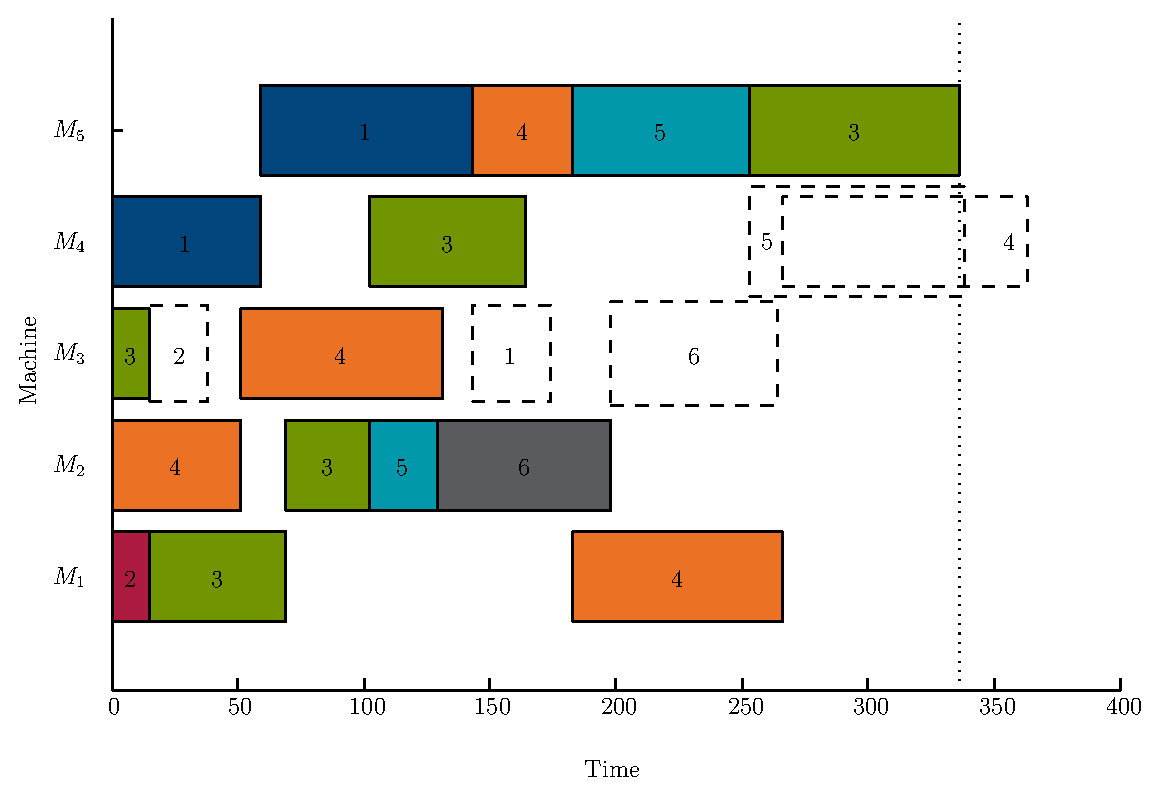
\includegraphics[width=\textwidth]{jssp_example}
\caption[Gantt chart of a partial \JSP\ schedule]{Gantt chart of a partial \JSP\ schedule after 15 dispatches: Solid and dashed boxes represent $\vchi$ and $\mathcal{R}^{(16)}$, respectively. Current $C_{\max}$ denoted as dotted line.}
\label{fig:example}
\end{figure}

\begin{figure}[p]\centering 
\noindent{\footnotesize\begin{tabbing}
\quad \quad \= 0\;\; \= \emph{Initialization}: Let $\vchi=\emptyset$ denote \\
\>  \> the current dispatching sequence. \\
\>1 \> {\bf for} \= $k := 1$ to $\ell=n\cdot m$ {\bf do} \emph{(at each dispatch iteration)}\\ 
\>2 \>\> {\bf for} \= $J_j\in \mathcal{R}^{(k)}\subset \mathcal{J}$ {\bf do} \emph{(inspect ready-list)} \\
\>3 \>\>\>  $I_j^{DR}\leftarrow \text{DR}\left([\vchi,j],Y\right)$ \emph{(priority $J_j$)}\\
\>4 \>\> {\bf od} \\
\>5 \>\> $j^*\leftarrow \argmax_{j\in \mathcal{R}^{(k)}}\{I_j^{DR}\}$ \emph{(choose highest priority)} \\
\>6 \>\> $\chi_k \leftarrow j^*$ \emph{(dispatch $j^*$)}\\
\>7 \> {\bf od} \\
\>8 \> $C_{max} \leftarrow Y(\vchi)$ \emph{(makespan)}
\end{tabbing}}
\caption{Pseudo code for constructing a \JSP\ sequence using a dispatching rule (DR) for a fixed construction heuristic (CH).}\label{fig:pseudocode}
\end{figure}


Henceforth, a \emph{sequence} will refer to the sequential ordering of the dispatches of tasks to machines, i.e., $(j,a)$; the collective set of allocated tasks to machines, which is interpreted by its sequence, is referred to as a \emph{schedule}; a \emph{scheduling policy} will pertain to the manner in which the sequence is manufactured for an (near) optimal schedule: be it a SDR such as MWR or via evolutionary search, etc. 

\section{Single-based priority dispatching rules}\label{sec:SDR}
\emph{Dispatching rules} (DR) are of a construction heuristics, where one starts with an empty schedule and adds sequentially on one operation (or task) at a time. Namely, at each time step $k$, an operation is dispatched which has the highest priority of the ready-list, \mbox{$\mathcal{R}^{(k)}\subset\mathcal{J}$}, i.e., the jobs who still have operations unassigned. If there is a tie, some other priority measure is used. 

A \emph{single-based priority dispatching rule}(SDR), or simple priority dispatching rule, is a function of features of the jobs and/or machines of the schedule. The features can be constant or vary throughout the scheduling process. For instance, the priority may depend on job processing attributes, such as which job has, 
\begin{description}
\item[Shortest immediate processing time (SPT)] \hfill \\
greedy approach to finish shortest tasks first,  
\item[Longest immediate processing time (LPT)] \hfill \\
greedy approach to finish largest tasks first, 
\item[Least work remaining (LWR)] \hfill \\
whose intention is to complete jobs advanced in their pro\-gress, i.e., minimising the ready-list $\mathcal{R}$,
\item[Most work remaining (MWR)] \hfill \\
whose intention is to accelerate the processing of jobs that require a great deal of work, yielding a balanced progress for all jobs during dispatching, however in-process inventory can be high.
\end{description}
These rules are the ones most commonly applied in the literature due to their simplicity and effectiveness, %\citep[cf.][]{Haupt89,Panwalkar77}
therefore they will be referenced throughout the dissertation. 
However there are many more available, e.g., randomly selecting an operation with equal possibility (RND); minimum slack time (MST); smallest slack per operation (S/OP); and using the aforementioned dispatching rules with predetermined weights. A survey of more than 100 of such rules are presented in \citet{Panwalkar77}, however the reader is referred to an in-depth survey for SDRs by \citet{Haupt89}. 

%Haupt89:
%Among the rules with job processing information, SPT is the most known, the most applied, and yet one of the most efficient rules. In line with LPT, it requires the lowest information amount, since only operation data (not job data) from the local queue (not from other queues) are needed.
%LWR give preference to jobs the work completed of which is rather advanced. Thus, they can be regarded as value-oriented rules selecting jobs with a high fraction of their value added or cumulative value to their total value.
% The intent of MWR is to speed up jobs with large processing work resulting in a well-balanced work progress of all jobs, at the expense of a high volume of in-process inventory, while LWR tend to reduce the number of jobs in the shop.

To summarise, SDRs assign an index to each job of the ready-list waiting to be scheduled, and are generally only based on few features and simple mathematical operations. 

%Haupt89:
%Among the rules with job processing information, SPT is the most known, the most applied, and yet one of the most efficient rules. In line with LPT, it requires the lowest information amount, since only operation data (not job data) from the local queue (not from other queues) are needed.
%LWR give preference to jobs the work completed of which is rather advanced. Thus, they can be regarded as value-oriented rules selecting jobs with a high fraction of their value added or cumulative value to their total value.
% The intent of MWR is to speed up jobs with large processing work resulting in a well-balanced work progress of all jobs, at the expense of a high volume of in-process inventory, while LWR tend to reduce the number of jobs in the shop.

\section{Features for \jsp}\label{sec:features}
A DR may need to perform a one-step look-ahead and observes features of the partial schedule to make a decision, for example by observing the resulting temporal makespan. These emanated observed features are sometimes referred to as an \emph{after-state} or \emph{post-decision state}. 

Features are used to grasp the essence of the current state of the schedule. Temporal scheduling features applied in this dissertation for a job $J_j$ to be dispatched on machine $M_a$ are given in \cref{tbl:features}. 
Note, from a job-oriented viewpoint, for a job already dispatched $J_j\in\mathcal{J}$ the corresponding set of machines now processed is $\mathcal{M}_j\subset\mathcal{M}$. Similarly from the machine-oriented viewpoint, $M_a\in\mathcal{M}$ with corresponding $\mathcal{J}_a\subset\mathcal{J}$. 

The features of particular interest were obtained from inspecting the aforementioned SDRs from \cref{sec:SDR}:  
\phiJobRelated\ and \phiMacRelated\ are job-related and machine-related attributes of the current schedule, respectively. 

Some features are directly observed from the partial schedule, such as the job- and machine-related features. 
In addition there are flow-related, \phiFlowRelated, which measure the influence of idle time on the schedule, 
and current makespan-related, \phiScheduleRelated.

Note that \phiLocalRelated\ are only based on the current step of the schedule, i.e., schedule's \emph{local features}, and might not give an accurate indication of how it will effect the schedule in the long run. Therefore, a set of features are needed to estimate the schedule's overall performance, referred to as its \emph{global features}. The approach here is to use well known SDRs, \phiSDRRelated, as a benchmark by retrieving what would the resulting $C_{\max}$ would be given if that SDR would be implemented from that point forward. Moreover, random completion of the partial schedule are implemented, here \phiRND\ corresponds to 100 random rollouts, which can be used to identify which features $\vphi$ are promising on a long-term basis.  

All of the features vary throughout the scheduling process, w.r.t. operation belonging to the same time step $k$, save for \phitotalProc\ which varies between jobs; \phistep\ to keep track of features' evolution w.r.t. the scheduling process; and \phiwrmTotal\ which is static for a given problem instance, but used for normalising other features, such as work-remaining based (\phiwrmJob\ and \phiwrmMac) or makespan-based (\phiGlobalRelated) ones.
In addition, \phimac, is reported in order to distinguish which features are in conflict with each other.

\begin{table} \centering 
  \caption[Feature space $\mathcal{F}$ for \JSP]{Feature space $\mathcal{F}$ for \JSP\ where job $J_j$ on machine $M_a$ given the resulting temporal schedule after dispatching $(j,a)$.}
  \label{tbl:features}
   {\footnotesize
 \centering
 \renewcommand{\arraystretch}{1.5}
  \begin{tabular}{clll}
	\toprule
  $\vphi$ & Feature description   & Mathematical formulation & Shorthand  \\ 
  %\hline  \multicolumn{4}{c}{\textbf{Local features}}  \\
  \midrule
  \multicolumn{4}{c}{\textbf{job related}}\\
  \phiproc         & job processing time                       & $p_{ja}$   & 
  proc         \\
  \phistartTime    & job start-time                            & $x_s(j,a)$ & 
  startTime    \\
  \phiendTime      & job end-time                              & $x_e(j,a)$ &
  endTime      \\
  \phiarrivalTime  & job arrival time                          & $x_e(j,a-1)$&
  arrival      \\ 
  \phiwait         & time job had to wait                      & 
  $x_s(j,a)-x_e(j,a-1)$ & 
  wait         \\   
  \phijobTotProcTime    & total processing time for job             & 
  $\sum_{a\in \mathcal{M}}p_{ja}$ & 
  jobTotProcTime \\
  \phijobWrm       & total work remaining for job              & 
  $\sum_{a'\in\mathcal{M}\setminus \mathcal{M}_{j}}p_{ja'}$ & 
  jobWrm       \\
  \phijobOps       & number of assigned operations for job     & 
  $|\mathcal{M}_j|$ & 
  jobOps       \\ 
  \midrule
  \multicolumn{4}{c}{\textbf{machine related}}\\
  \phimacFree      & when machine is next free                 & 
  $\max_{j'\in \mathcal{J}_a} \{x_e(j',a)\}$ &
  macFree      \\
  \phimacTotProcTime    & total processing time for machine    & 
  $\sum_{j\in \mathcal{J}}p_{ja}$ & 
  macTotProcTime \\
  \phimacWrm       & total work remaining for machine          & 
  $\sum_{j'\in\mathcal{J}\setminus \mathcal{J}_{a}}p_{j'a}$ &  
  macWrm       \\
  \phimacOps       & number of assigned operations for machine & 
  $|\mathcal{J}_a|$ & 
  macOps       \\
  \phireducedSlack & change in idle time by assignment         & 
  $\Delta s(a,j)$ &
  reducedSlack \\
  \phimacSlack        & total idle time for machine               & 
  $\sum_{j'\in \mathcal{J}_a}s(a,j')$ &
  macSlack        \\
  \phiallSlack   & total idle time for all machines          & $\sum_{a'\in 
    \mathcal{M}}\sum_{j'\in \mathcal{J}_{a'}}s(a',j')$                    & 
  allSlack   \\
  \phimakespan     & current makespan                          &
  $\max_{(j',a')\in \mathcal{J} \times \mathcal{M}_{j'}}\{x_f(j',a')\}$ & 
  makespan     \\
  \midrule
  \multicolumn{4}{c}{\textbf{final makespan related}}\\
  \phiSPT & final makespan using SPT & $ C_{\max}^{\SPT}$ & SPT \\
  \phiLPT & final makespan using LPT & $ C_{\max}^{\LPT}$ & LPT \\
  \phiLWR & final makespan using LWR & $ C_{\max}^{\LWR}$ & LWR \\
  \phiMWR & final makespan using MWR & $ C_{\max}^{\MWR}$ & MWR \\
  $\phiRND$ & final makespans using 100 random rollouts & $ 
  \{C_{\max}^{\RND}\}_{i=1}^{100}$ & \\  
  \phiRNDmean & mean for $\phiRND$ & $\Exp{\phiRND}$ & RNDmean \\  
  \phiRNDstd & standard deviation for $\phiRND$ & 
  $\sqrt{\Exp{\phiRND^2}-\Exp{\phiRND}^2}$ &
  RNDstd \\
  \phiRNDmin & minimum value for $\phiRND$ & $\min\{\phiRND\}$ & RNDmin \\  
  \phiRNDmax & maximum value for $\phiRND$ & $\max\{\phiRND\}$ & RNDmax \\  
  \bottomrule
  \end{tabular}
}
 %Feature description for job $J_j$ on machine $M_a$ given current temporal schedule, where the set of jobs already dispatched are $J\subset\mathcal{J}$ on corresponding set of machines $\mathcal{M}_j\subset\mathcal{M}$

\end{table}



\section{Composite dispatching rules}\label{sec:CDR}
\citet{Jayamohan04} showed that a careful combination of dispatching rules can perform significantly better. These are referred to as \emph{composite dispatching rules} (CDR), where the priority ranking is an expression of several SDRs. For instance, optimising \JSP\ w.r.t. $L_{max}$ for one machine\ \cite[see. chapter 14.2]{Pinedo08}, one can combine SDRs that are optimal for a different criteria of problem instances, which complement each other as a CDR, e.g., combining the SDRs 
WSPT (SPT weighted w.r.t. $\mathcal{J}$), ``which is optimal when all release dates and due dates are zero,'' 
and minimum slack first (MS), ``which is optimal when all due dates are sufficiently loose and spread out,'' 
one gets the CDR apparent tardiness cost (ATC) which can work well on a broader set of problem instances than the original SDRs by themselves.

CDRs can deal with greater number of features and more complicated form, in short, CDR are a combination of several SDRs. For instance let CDR be comprised of $d$ SDRs, then the index $I$ for job $J_j$ using CDR is, 
\begin{equation}
I_j^{CDR} = \sum_{i=1}^d w_i \cdot \text{DR}^i(\vphi_j)
\end{equation}
where $w_i>0$ and $\sum_{i=0}^d w_i = 1$, then $w_i$ gives the \emph{weight} of the influence of $\text{DR}^i$ (which could be SDR or another CDR) to CDR. Note, each $\text{DR}^i$ is a function of the job $J_j$'s feature state $\vphi_j$.

\subsection{Blended dispatching rules}
Since each DR yield a priority index $I^{DR}$ then it is easy to translate its index as a  performance measure $a$, i.e., $a:~I^{DR}\mapsto \mathcal{Y}$. Then it is possible to combine several performance measures into a single DR, these are referred to as \emph{blended dispatching rules} (BDR), where an overall blended priority index $P$ is defined as 
\begin{equation}
P_j = \sum_{i=1}^d w_i \cdot a_i 
\end{equation}
where $w_i>0$ and $\sum_{i=0}^d w_i = 1$, then $w_i$ gives the weight of the proportional influence of performance measure $a_i$ (based on some SDR or CDR) to the overall priority. 

Generally the weights $\vec{w}$ chosen by the algorithm designer a priori. 
A more sophisticated approach would to learn have the algorithm discover these weights autonomously, for instance via evolutionary search or ordinal regression, to be discussed in \cref{ch:esmodels} and \cref{ch:prefmodels}, respectively.

\subsection{Automated discovery of dispatching rules}
\citet{Monch13} stress the importance of automated discovery of DRs and named several of successful implementations in the field of semiconductor wafer fabrication facilities, however this sort of investigation is still in its infancy and subject for future research.

A recent editorial of the state-of-the-art approaches in advanced dispatching rules for large-scale manufacturing systems by \citet{Chen13} points out that:
\begin{quote}
[..] most traditional dispatching rules are based on historical data. With the emergence of data mining and on-line analytic processing, dispatching rules can now take predictive information into account.
\end{quote}
implying that there has not been much automation in the process of discovering new dispatching rules, which is the ultimate goal of this dissertation, i.e., automate creating optimisation heuristics for scheduling. 

With meta heuristics one can use existing DRs and use for example portfolio-based algorithm selection \citep{Rice76,Gomes01}, either based on a single instance or class of instances \citep{Xu07} to determine which DR to choose from. 
Instead of optimising which algorithm to use under what data distributions, such as the case of portfolio algorithms, the approach taken in this dissertation is more similar to that of \emph{meta learning} \citep{Vilalta02} which is the study of how learning algorithms can be improved, i.e., exploiting their strengths and remedy their failings, in order for a better algorithm design. Thus creating an adaptable learning algorithm that dynamically finds the appropriate dispatching rule  to the data distribution at hand. 

\citet{Kalyanakrishnan11} point out that meta learning can be very fruitful in reinforcement learning, and in their experiments they discovered some key discriminants between competing algorithms for their particular problem instances, which provided them with a hybrid algorithm which combines the strengths of the algorithms.

\citet{Nguyen13} proposed a novel iterative dispatching rules (IDR) for \JSP\ which learns from completed schedules in order to iteratively improve new ones. At each dispatching step, the method can utilise the current feature space to \emph{correctify} some possible \emph{bad} dispatch made previously (sort of reverse lookahead).
Their method is straightforward, and thus easy to implement and more importantly, computationally inexpensive, although \citeauthor{Nguyen13} stress that there still remains room for improvement. 

\citet{Korytkowski13} implement ant colony optimisation to select the best DR from a selection of nine DRs for \JSP\ and their experiments showed that the choice of DR do affect the results and that for all performance measures considered it was better to have all of the DRs to choose from rather than just a single DR at a time. 
Similarly, \citet{Lu13} investigate eleven SDRs for \JSP\ to create a pool of thirty three CDRs that strongly outperformed the ones they were based on, which is intuitive since where one SDR might be failing, another could be excelling, hence combining them should yield a better CDR. \citeauthor{Lu13} create their CDRs with multi-contextual functions (MCF) based either on machine idle time or job waiting time, so one can say that the CDRs are a combination of those two key features of the schedule and then the basic DRs. However, there are no combinations of the basic DR explored, only machine idle time and job waiting time.  
\citet{Yu13} used priority rules to combine twelve existing DRs from the literature, in their approach they had forty eight priority rules combinations, yielding forty eight different models to implement and test. This is a fairly ad hoc solution and there is no guarantee the optimal combination of DRs is found. 

\clearpage
\section{Rice's framework for \jsp}\label{sec:rice:jsp}
\citeauthor{Rice76}'s framework for algorithm selection (discussed in \cref{sec:rice}) has already been formulated for \jsp\ \citep[cf.][]{SmithMilesLion3,SmithMilesLion5,InRu12}, as follows, 
\begin{description} 
\item[Problem space] $\mathcal{P}$ is defined as the union of $N$ problem instances consisting of processing time and ordering matrices,
\begin{equation} 
\mathcal{P}=\left\{(p_{ja}^{(i)},\vsigma_j^{(i)})\;\big|\;J_j\in\mathcal{J},\;M_a\in\mathcal{M}\right\}_{i=1}^{N}
\end{equation}
Problem generators for $\mathcal{P}$ are given in \cref{ch:genprobleminstances}.
\item[Feature space] $\mathcal{F}$ which is outlined in \cref{sec:features}. Note, these are not the only possible set of features, however, the local feature, \phiLocalRelated, are built on the work by \cite{InRu11a,SmithMilesLion3} and deemed successful in capturing the essence of a \jsp\ data structure;
\item[Algorithm space] $\mathcal{A}$ is simply the scheduling policies under consideration, e.g., SDRs from \cref{sec:SDR},
\begin{equation}
\mathcal{A}=\left\{\text{SPT,~LPT,~LWR,~MWR}\dotsc\right\}
\end{equation} 
\item[Performance space] $\mathcal{Y}$ is based on the resulting $C_{\max}$, defined by \cref{eq:makespan}. The optimum makespan is denoted $C_{\max}^{\text{opt}}$, and the makespan obtained from the scheduling policy $A\in\mathcal{A}$ under inspection by $C_{\max}^{A}$. Since the optimal makespan varies between problem instances the performance measure is the following, 
\begin{equation}\label{eq:rho}
\rho=\frac{C_{\max}^{A}-C_{\max}^{opt}}{C_{\max}^{\text{opt}}}\cdot 100\%
\end{equation}
which indicates the \namerho. Thus $\mathcal{Y}$ is the following, 
\begin{equation}
\mathcal{Y}=\left\{\rho_i\right\}_{i=1}^{N}
\end{equation}
\end{description}
The mapping $Y:\;\mathcal{A}\times\mathcal{F} \mapsto \mathcal{Y}$ is the step-by-step construction heuristic introduced in \cref{sec:CH}. %ch.2
\HeaderQuote{If it had grown up, it would have made a dreadfully ugly child; but it makes rather a handsome pig, I think.}{Alice} 

\chapter{Problem generators}\label{ch:genprobleminstances} 

\FirstSentence{S}{ynthetic problem instances for } \JSP\ and \FSP\  will be used  throughout this dissertation. The  problem spaces are detailed in the \cref{sec:data:JSP,sec:data:FSP} for \JSP\ and \FSP, respectively. Moreover, a brief summary is given in \cref{tbl:data}.
Following the approach in \citet{Whitley}, difficult problem instances are not 
filtered out beforehand. %, although they will be specifically addressed in 
%\cref{ch:defdifficulty}. 
The problem spaces for \cref{Papers} are summarised in 
\cref{tbl:papers:problems}. Note, that the problem generators in 
\cref{InRu14,InRu15a,InRu15b} are the same as described here.

\begin{table}[b]
    \caption{\JSP\ and  \FSP\ problems spaces used in \cref{Papers}}
    \label{tbl:papers:problems}
    \noindent 
    \begin{minipage}{\textwidth}\centering
    {\setlength{\tabcolsep}{3pt}
    \begin{tabular}{c l l l l}\toprule
      Paper & Problem & $I=[u_1,u_2]$\footnote{Processing times are uniformly
        distributed from an interval $I=[u_1,u_2]$, i.e., 
        $\vec{p}\sim\mathcal{U}(u_1,u_2)$.} & size ($n\times m$) & name \\ 
        \midrule
      \ref{InRu11a} & \JSP & $[1,100], [50,100]$ & $6\times6$ & j.rnd, j.rndn\\
      \ref{InRu12} & \JSP & $[1,200]$ & $6\times 6$ & j.rnd \\
      \ref{InRu14} & \JSP, \FSP & $[1,99],[45,55]$ & $6\times5,10\times10$ & 
      j.rnd, j.rndn, f.rnd, f.rndn, f.jc\\
      \ref{InRu15a} & \JSP & $[1,99],[45,55]$ & $6\times5$ & j.rnd, j.rndn\\
      \ref{InRu15b} & \JSP, \FSP & $[1,99],[45,55]$ & $10\times10$ & 
      j.rnd, j.rndn, f.rnd\\
      \ref{InRu15c} & \JSP, \FSP & $[1,99],[45,55]$ & $6\times5,10\times10$ & 
      j.rnd, j.rndn, f.rnd\\
      \bottomrule
    \end{tabular}}
    \end{minipage}
\end{table}


Although real-world instances are desirable, unfortunately they are scarce. 
Hence in some experiments (mainly in \cref{ch:orlibrobust}), problem instances 
from OR-Library maintained by \citet{ORlibrary} will be used as benchmark 
problems. They are detailed in \cref{sec:data:orlib}. 

It is noted, that some of the instances are also simulated, but the majority 
are based on real-world instances, albeit sometimes simplified. 
%\citet{Panwalkar77} reports an extensive survey of 36 research papers in scheduling, most experiments are based on simulated data, and its verification on real-world data would be desirable, but missing. 

\section{\Jsp}\label{sec:data:JSP}
Problem instances for \JSP\ are generated stochastically by fixing the number of jobs and machines and 
discrete processing time are i.i.d. and sampled from a discrete uniform distribution. % from the interval $I=[u_1,u_2]$, i.e., $\vec{p}\sim \mathcal{U}(u_1,u_2)$. 
Two different processing times distributions were explored, namely,
\begin{description}
	\item[\Jrnd] \jrnd{n}{m} \hfill \\ where $\vec{p}\sim\mathcal{U}(1,99)$;
	\item[\Jrndn] \jrndn{n}{m} \hfill \\ where $\vec{p}\sim\mathcal{U}(45,55)$.
\end{description}
The machine ordering is a random permutation of all of the machines in the \jsp. 
For each \JSP\ class $N_{\train}$  and $N_{\test}$ instances were 
generated for training and testing, respectively. Values for $N$ are given in 
\cref{tbl:data}. 

Although in the case of \jrnd{n}{m}\ this may be an excessively large range for 
the uniform distribution, it is however, chosen in accordance with the 
literature \citep{Demirkol98} for creating synthesised $Jm||C_{\max}$ problem 
instances. 

In order to inspect the impact of any slight change within the problem spaces, 
two mutated versions were created based on \jrnd{n}{m}, namely, 
\begin{description}
	\item[\JrndJ] \jrndJ{n}{m} \hfill \\ where the first job, $J_1$, is always twice as long as its random counterpart, i.e.,\linebreak
	$\tilde{p}_{1a}=2\cdot p_{1a}$, where $p\in$\jrnd{n}{m}, for all $M_a\in\mathcal{M}$. 
	\item[\JrndM] \jrndM{n}{m} \hfill \\ where the first machine, $M_1$, is always twice as long as its random counterpart, i.e.,\linebreak
	$\tilde{p}_{j1}=2\cdot p_{j1}$, where $p\in$\jrnd{n}{m}, for all $J_j\in\mathcal{J}$. 
\end{description}
Therefore making job $J_1$ and machine $M_1$ bottlenecks for \jrndJ{n}{m} and 
\jrndM{n}{m}, respectively.

\citet{Hildebrandt2010} argue that the randomly generated problem 
instances aren't a proper representative for real-world long-term \jsp\   
applications, e.g., by the narrow choice of release-dates, yielding schedules 
that are overloading in the beginning phases. However, as stated in
\cref{ch:scheduling}, release-dates constraints won't be considered here.
In addition, w.r.t. the machine ordering, one could look into a 
subset of \JSP\ where the machines are partitioned into two (or more) sets, 
where all jobs must be processed on the machines from the first set (in some 
random order) before being processed on any machine in the second set, commonly 
denoted as $Jm|2\textrm{sets}|C_{\max}$ problems, but as discussed in 
\cite{orlib_swv} this family of \JSP\ is considered `hard' (w.r.t. relative 
error from best known solution) in comparison with the `easy' or 
`unchallenging' family with the general $Jm||C_{\max}$ set-up. % ath. 
%Holtsclaw96 vitnar í orlib_swv um easy-hard pælinguna
This is in stark contrast to \citet{Whitley} whose findings showed that 
structured $Fm||C_{\max}$ were much easier to solve than completely random 
structures. 
Intuitively, an inherent structure in machine ordering should be exploitable 
for a better performance.  However, for the sake of generality, a random 
structure is preferred as they correspond to difficult problem instances in the 
case of \JSP. Whereas, structured problem subclasses will be explored for 
\FSP.  

\section{\Fsp}\label{sec:data:FSP}
Problem instances for \FSP\  are generated using \citet{Whitley} problem 
generator.\footnote{Both code, written in \texttt{C++}, and problem instances 
used in their experiments can be found at: 
\url{http://www.cs.colostate.edu/sched/generator/}}
There are two fundamental types of problem classes: non-structured versus 
structured.

Firstly, there are two `conventional' random (i.e. non-structured) problem 
classes for \FSP\  where processing times are i.i.d. and uniformly distributed, 
\begin{description}
	\item[\Frnd]  \frnd{n}{m} \hfill \\
	where $\vec{p}\sim\mathcal{U}(1,99)$ whose instances are equivalent to \cite{Taillard1993}\footnote{\citeauthor{Taillard1993}'s generator is available from the OR-Library.};
	\item[\Frndn]  \frndn{n}{m} \hfill \\
	where $\vec{p}\sim\mathcal{U}(45,55)$.
\end{description}
In the \JSP\ context \frnd{n}{m}\ and \frndn{n}{m}\ are analogous to \jrnd{n}{m}\ and \jrndn{n}{m}, respectively.  

Secondly, there are three structured problem classes of \FSP\  which are modelled after real-world \emph{characteristics} in \fsp\ manufacturing, namely, 
\begin{description}
	\item[\Fjc] \fjc{n}{m} \hfill \\
	where $\vec{p}$ is dependent on job index, however, independent of 
	machine index. 
	\item[\Fmc]  \fmc{n}{m} \hfill \\
	where $\vec{p}$ is dependent on machine index, however, independent of 
	job index. 
	\item[\Fmxc]  \fmxc{n}{m} \hfill \\
	where $\vec{p}$ is dependent on machine and job indices. 
\end{description} 
In all cases, the (job, machine or mixed) correlation can be of degree 
$0\leq\alpha\leq1$. 
When $\alpha=0.0$ the problem instances closely correspond to \frnd{n}{m}, 
hence the degree of $\alpha$ controls the transition of random to structured. 
Let's assume $\alpha=1$.

An example of distribution of processing times are depicted in 
\cref{fig:fsp:structure}, where machine indices are on the horizontal axis, job 
indices are shape-coded, and their corresponding processing times, $p_{ja}$, 
are on the vertical axis.

\begin{figure}\centering 
  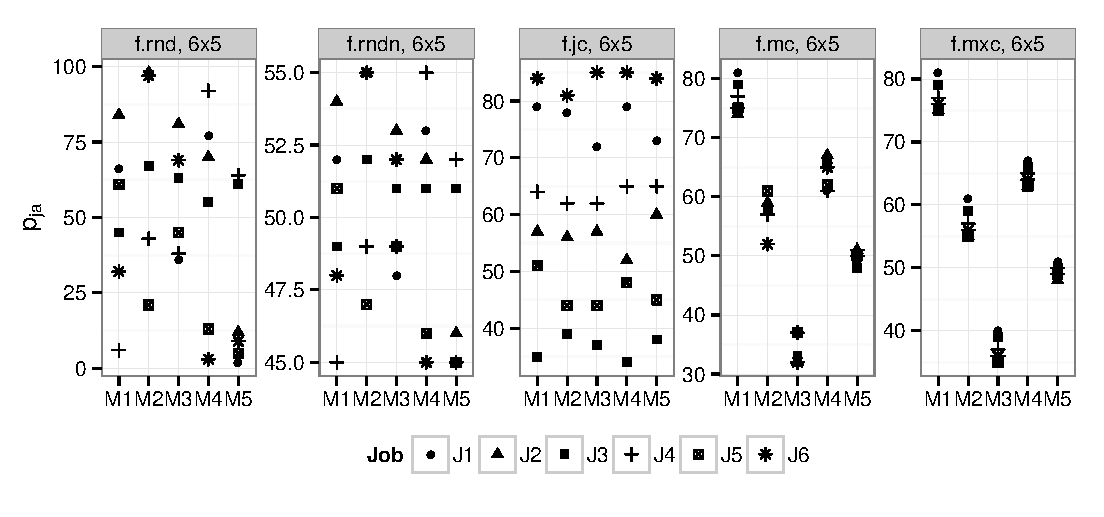
\includegraphics[width=\textwidth]{proctimes.pdf}
  \caption[Examples of job processing times of different \FSP\ structures 
  ]{Examples of job processing times for $6\times5$ of different \FSP\ 
  structures}
  \label{fig:fsp:structure}
\end{figure}

For each \FSP\  class $N_{\train}$  and $N_{\test}$ instances were 
generated for training and testing, respectively. Values for $N$ are given in 
\cref{tbl:data}. 

\begin{table}[t]\centering
	\caption{Problem space distributions used in experimental studies. 
    %Note, problem instances are synthetic and each problem space is i.i.d.
    }\label{tbl:data}
    {\renewcommand{\arraystretch}{1.5}
    \begin{tabular}{llcccl}\toprule
& name & size ($n\times m$) & $N_{\train}$ & $N_{\test}$ & note 
\\ \midrule
\multirow{8}{*}{\rot{\JSP}}
& \jrnd{6}{5}   &$6\times5$ & 500 & 500 & random \\
& \jrndn{6}{5}  &$6\times5$ & 500 & 500 & random-narrow \\
& \jrndJ{6}{5}  &$6\times5$ & 500 & 500 & random with job variation \\
& \jrndM{6}{5}  &$6\times5$ & 500 & 500 & random with machine variation \\
& \jrnd{10}{10} &$10\times10$& 300 & 200 & random \\
& \jrndn{10}{10}&$10\times10$& 300 & 200 & random-narrow \\ 
& \jrndJ{10}{10} &$10\times10$& 300 & 200 & random with job variation\\
& \jrndM{10}{10} &$10\times10$& 300 & 200 & random with machine variation\\
\midrule
\multirow{6}{*}{\rot{\FSP}}
& \frnd{6}{5}  & $6\times5$ & 500 & 500 & random \\ 
& \frndn{6}{5} & $6\times5$ & 500 & 500 & random-narrow \\ 
& \fjc{6}{5}   & $6\times5$ & 500 & 500 & job-correlated \\ 
& \fmc{6}{5}   & $6\times5$ & 500 & 500 & machine-correlated \\ 
& \fmxc{6}{5}  & $6\times5$ & 500 & 500 & mixed-correlation \\ 
& \frnd{10}{10}& $10\times10$ & 300 & 200 & random \\ 
\bottomrule
\end{tabular}}
\end{table}

\section{Benchmark problem suite}\label{sec:data:orlib}
A total of 82 and 31 benchmark problems for \JSP\ and \FSP, respectively, were 
obtained from the Operations Research Library (OR-Library) maintained by 
\citet{ORlibrary} and summarised in \cref{tbl:data:orlib}. 
Given the high problem dimensions of some problems, the optimum is not known, 
hence in those instances \cref{eq:rho} will be reporting  deviation from the 
latest best known solution (BKS) from the literature, reported by 
\citet{Jain99,orlibJSP}, and for \FSP\  consult \citet{orlibFSP}.

\subsection*{\Jsp\ OR-Library}
\citet{orlib_ft} had one of the more notorious benchmark problems for \JSP, and 
computationally expensive. However, now these instances have been solved to 
optimality. 
Similar to the synthetic \JSP\ problem spaces discussed earlier, 
\citet{orlib_abz} introduce five \JSP\ instances with a random machine ordering 
and processing times $\vec{p}\sim\mathcal{U}(50,100)$, for  dimensions 
$10\times10$ and $20\times15$. 
Likewise, \citet{orlib_yn} consists of four $20\times20$ random 
problem instances, where $\vec{p}\sim\mathcal{U}(10,50)$.
\citet{orlib_swv} introduce a set of \JSP\ problems where 
$\vec{p}\sim\mathcal{U}(1,100)$. There are a total of five problems in four 
dimension classes 
\begin{enumerate*}
  \item $20\times10$ %(\texttt{swv01-swv05})
  \item $20\times15$ %(\texttt{swv06-swv10})
  \item $50\times10$ %(\texttt{swv11-swv15})
  \item $50\times10$ %(\texttt{swv16-swv20})
\end{enumerate*}
Where the first three classes are considered `{hard}' and the last one as 
`{easy}'. Easy problems are ones corresponding to random machine ordering, 
whereas hard problems are partitioned in such a way the jobs must be processed 
on the first half of the machines before starting on the second half, i.e., 
$Jm|\text{2sets}|C_{\max}$.
\citet{orlib_orb} introduced ten problem instances of $10\times10$ \JSP\ where 
generated such that the machine ordering was chosen by random users in order to 
make them `difficult.' Moreover, the processing times were drawn at random, 
and the distribution that had the greater gap between its optimal value and 
standard lower bound was chosen. 

\subsection*{\Fsp\ OR-Library}
For the \FSP\ benchmarks, \citet{orlib_hel} introduces two deterministic 
instances based on `many-machine version of book-printing,' where processing 
times for $n\in\{20,100\}$ jobs and $m=10$ machines are relatively short, 
i.e., $p_{ja}\in\{0,..,9\}$. \citet{orlib_car} however, comprises of eight 
problems (of various dimension) where there is high variance in processing 
times, presumably $\vec{p}\sim\mathcal{U}(1,1000)$. 
\citet{orlib_rec} argues that completely random problem instances are unlikely 
to occur in practice. However, only the random instances they used (type C) are 
reported in the OR-Library, for a total of 42 problem instances with processing 
times following a uniform distribution, $\vec{p}\sim\mathcal{U}(1,100)$, of 
dimensions varying from $20\times5$ to $75\times20$, although \cite{orlibFSP} 
omitted \ProblemSpace[75 \times 20]{reC} instances in their comparison.

\begin{table}\centering
\noindent
\begin{minipage}{\textwidth}
  \caption{Benchmark problems from OR-Library used in experimental studies.}
  \label{tbl:data:orlib}
  \begin{tabular}{llrrll}\toprule
    & name & $n\times m$ & $N_{\test}$ & note & shorthand  \\
    \midrule \multirow{6}{*}{\rot{\JSP}}
    &\ProblemSpace{ft} & various &  3 &\citet{orlib_ft} & 
    \texttt{ft06,ft10,ft20}\\
    &\ProblemSpace{la} & various & 40 &\citet{orlib_la} & 
    \texttt{la01-la40}     \\
    &\ProblemSpace{abz}& various &  5 &\citet{orlib_abz}& 
    \texttt{abz05-abz09}   \\
    &\ProblemSpace{orb}& $10\times10$& 10 &\citet{orlib_orb}& 
    \texttt{orb01-orb10}\\
    &\ProblemSpace{swv}& various & 20 &\citet{orlib_swv}&\texttt{swv01-swv20}\\
    & \ProblemSpace{yn} & $20\times20$& 4  &\citet{orlib_yn} & 
    \texttt{yn01-yn04}\\
    \midrule \multirow{3}{*}{\rot{\FSP}}
    &\ProblemSpace{car}& various &  8 & \citet{orlib_car} & \texttt{car1-car8} 
    \\
    &\ProblemSpace{hel}& various &  2 & \citet{orlib_hel} & \texttt{hel1,hel2}  
    \\
    &\ProblemSpace{reC}& various & 21 & \citet{orlib_rec}\footnote{Only 
    odd-numbered
        instances in \texttt{rec01-rec42} are given, since the even-numbered 
        instances are obtained from the previous instance by just reversing the 
        processing order of each job; the optimal value of each odd-numbered 
        instance and its even-numbered counterpart is the same.}  
    & \texttt{reC01-reC42}\\
    \bottomrule
\end{tabular}

\end{minipage}
\end{table}
 %ch.3
\HeaderQuote{Sentence first -- verdict afterwards.}{The Queen}

\chapter{Problem difficulty}\label{ch:defdifficulty} 

%\begin{abstract} 
%Many heuristic methods have been proposed for the \jsp\ scheduling problem. Different solution methodologies outperform other depending on the particular problem instance under consideration. Therefore, one is interested in knowing how the instances differ in structure and determine when a particular heuristic solution is likely to fail and explore in further detail the causes. In order to achieve this, we seek to characterise features for different difficulties. Preliminary experiments show there are different significant features that distinguish between easy and hard \jsp\ problem, and that they vary throughout the scheduling process. 
%The insight attained by investigating the relationship between problem structure and heuristic performance can undoubtedly lead to better heuristic design that is tailored to the data distribution under consideration.
%\end{abstract}

\FirstSentence{P}{roblem structure and heuristic effectiveness} are closely 
intertwined. When investigating the relation between the two, one can research 
what \citet{Corne10} call \emph{footprints}, which is an indicator how an 
algorithm generalises over a given instance space. This sort of investigation 
has also been conducted by \citet{Pfahringer00} under the alias 
\emph{landmarking}. 
% quote Corne10: ``such a footprint indicates how an algorithm's comparative performance generalises in instance space''
% quote Katie2009: ``Landmarking tries to directly characterise a domain by relating the performance to some learners -- the landmarkers -- to the performance of some other algorithm.''
From experiments performed by \citeauthor{Corne10}, it is evident that 
one-algorithm-for-all problem instances is not ideal, in accordance with no 
free lunch theorem \citep{Wolpert97nofree}. An algorithm may be favoured for 
its best overall performance, however, it is rarely the best algorithm 
available over various subspaces of the instance space.
Therefore, when comparing different algorithms one needs to explore how they perform w.r.t. the instance space, i.e., their footprint. That is to say, one can look at it as finding which footprints correspond to a subset of the instance space that works \emph{well} for a given algorithm, and similarly finding which footprints correspond to a subset of the instance space that works \emph{poorly} for a given algorithm. 

\clearpage

In the context of \jsp\ this corresponds to finding \emph{good} (makespan close to its optimum)  and \emph{bad} (makespan far off its optimum) schedules. Note, good and bad schedules are interchangeably referred to as \emph{easy} and \emph{hard} schedules (pertaining to the manner they are achieved), respectively. 

\citet{SmithMilesLion5} also investigate algorithm performance in instance space using footprints. The main difference between \citeauthor{Corne10} and \citeauthor{SmithMilesLion5} is how they discretise the instance space. In the case of \citeauthor{Corne10} they use \jsp\ and discretise manually between different problem instances; on one hand w.r.t. processing times, e.g.,  $\vec{p}\sim \mathcal{U}(10,20)$ versus $\vec{p}\sim \mathcal{U}(20,30)$ etc., and on the other hand w.r.t. number of jobs, $n$. 
They warn that footprinting can be uneven, so great care needs to be taken in 
how to discretise the instance space into subspaces. 
This is why we consider the random vs. random-narrow problem spaces in 
\cref{sec:data:JSP,sec:data:FSP}.

On the other hand, \citeauthor{SmithMilesLion5} use a completely automated 
approach. Using timetabling instances, they implement a self-organizing map 
(SOM) on the feature space to group similar problem instances together, that 
were both real world instances and synthetic ones using different problem 
generators. That way it was possible to plot visually the footprints for 
several algorithms.

Going back to the \jsp\ paradigm, then the interaction between processing time 
distribution and its permutation is extremely important, because it introduces 
hidden properties in the data structure making it \emph{easy} or \emph{hard} to 
schedule for the given algorithm. These underlying characteristics (i.e. 
features), define its data structure. A more sophisticated way of discretising 
the instance space is grouping together problem instances that show the same 
kind of feature behaviour, especially given the fact the learning models in 
\cref{ch:prefmodels} will be heavily based on feature pairs. Thereby making it 
possible to infer what sort of feature behaviour distinguishes  between 
\emph{good} and \emph{bad} schedules. 

Instead of searching through a large set of algorithms  and determining which 
algorithm is the most suitable for a given subset of the instance space, i.e., 
creating an algorithm portfolio, as is generally the focus in the current 
literature \citep{SmithMilesLion3,SmithMilesLion5,Corne10}, the focus of the 
experimental study in the subsequent \lcnamecref{sec:diff:easyhard}s
is rather on few simple algorithms, namely the SDRs described in 
\cref{sec:SDR}, i.e., we will limit the algorithm space to, 
\begin{equation}\label{eq:SDRset}
\mathcal{A}:=\{\text{SPT,~LPT,~LWR,~MWR}\}
\end{equation} 
and try to understand \emph{how} they work on the instance space, similar to 
\citet{Whitley}, who analysed the fitness landscape of several problem classes 
for a fixed algorithm. 

Depending on the data distribution, dispatching rules perform differently. 
A box-plot for \fullnamerho, using all problem spaces from \cref{tbl:data} are 
depicted in \cref{fig:SDR:boxplot}. 
As one can see, there is a staggering difference between the interaction of 
SDRs and their problem space. MWR is by far the best out of the four SDRs 
inspected for \JSP\ -- not only does it reach the known optimum most often but 
it also has the lowest worst-case factor from optimality. Similarly LWR for 
\FSP.

Although the same processing time distribution is used, there are some inherent structure in which MWR and LWR can exploit for \JSP\ and  \FSP, respectively, whereas the other SDRs cannot. However, \emph{all} of these dispatching rules are considered good and commonly used in practice and no one is better than the rest \citep{Haupt89}, it simply depends on the data distribution at hand. This indicates that some distributions are harder than others, and these \JSP\ problem generators simply favours MWR, whereas the \FSP\ problem generators favours LWR. 

\begin{figure}[p]
  \subcaptionbox{$6\times5$\label{fig:SDR:boxplot:6x5}}{
    \includegraphics[width=\textwidth]{{boxplotRho.SDR.6x5}.pdf}}
  \caption[Box-plots of \namerho, when applying SDRs]{Box-plots of \namerho, 
    when applying SDRs for all problem spaces in \cref{ch:genprobleminstances}.}
  \label{fig:SDR:boxplot}
\end{figure}
\begin{figure}[h]
  \ContinuedFloat 
  \subcaptionbox{$10\times10$\label{fig:SDR:boxplot:10x10}}{
    \includegraphics[width=\textwidth]{{boxplotRho.SDR.10x10}.pdf}}
  \caption{Continued.}
\end{figure}

\section{Distribution difficulty}
In \cref{InRu12}, a single problem generator was used to create  $N=1,500$ 
synthetic $6\times6$ \jsp\ problem instances, where 
$\vec{p}\sim\mathcal{U}(1,200)$ and $\vsigma$ was a random permutation. The 
experimental study showed that MWR works either well or poorly on a subset of 
the instances, in fact 18\% and 16\% of the instances were classified as 
\emph{easy} and \emph{hard} for MWR, respectively. 
Since the problem instances were na\"{i}vely generated, not to mention given 
the high variance of the data distribution, it is intuitive that there are some 
inherent structural qualities that could explain this difference in 
performance. The experimental study investigated the feature behaviours for 
these two subsets, namely, the easy and hard problem instances. For some 
features, the trend was more or less the same, which are explained by the 
common denominating factor, that all instances were sampled from the same 
problem generator. Whereas, those features that were highly correlated with the 
end-result, i.e., the final makespan, which determined if an instance was 
labelled easy or hard, then the significant features varied greatly between the 
two difficulties, which imply the inherent difference in data structure. 
Moreover, the study in gives support to that random problem instance generators 
are \emph{too} general and might not suit real-world applications. 
\citet{Whitley} argue that problem instance generator should be more 
structured, since real-world manufacturing environment is not completely 
random, but rather structured, e.g.,  job's tasks can be correlated or machines 
in the shop. \citeauthor{Whitley} propose a problem instance generator that 
relates to real-world \fsp\ attributes, albeit not directly modelled after 
real-world \fsp\ due to the fact that deterministic $Fm||C_{\max}$ is seldom 
directly applicable in practice \citep{Dudek92}. This is why \fjc{n}{m}, 
\fmc{n}{m} and \fmxc{n}{m} are also taken into consideration in 
\cref{sec:data:FSP}.

\section{Defining \emph{easy} versus \emph{hard} schedules} 
\label{sec:diff:easyhard}

It's relatively ad-hoc how to define what makes a schedule difficult. 
For instance, it could be sensible to define it in terms of how many Simplex 
iterations are needed to find an optimal schedule, using \emph{Branch and 
Bound}.\footnote{Branch and bound \citep{bnb} is a methodology in integer
    linear programming, where the original problem is branched into smaller sub 
    problems until it becomes easily solvable. Each sub problem has an lower 
    bound on its solution, found with LP-relaxation. Depending on the lower 
    bound, sub branches are systemically discarded, since they cannot contain 
    the optimal solution.} 
However, it showed that an increased amount of Simplex iterations 
didn't necessarily transcend to high $\rho$. 
If anything, it means there are many optimal (or near-optimal) solutions 
available, which causes the slow process of pruning branches of the tree, 
before reaching to a final incumbent solution. If that's the case, than that's 
promising for our instance, as it's likelier for an arbitrary algorithm to find 
a good solution. 
Intuitively, it's logical to use the schedule's objective to define the 
difficulty directly, i.e., inspecting \namerho. Moreover, since the SDRs from 
\cref{eq:SDRset} will be used throughout as a benchmark for subsequent models, 
the quantiles for $\rho$, using the SDRs on their training set will be used 
to differentiate between easy and hard instances. In particular, the 
classification is defined as follows, 
\begin{description}
  \item[Easy] schedules belong to the first quantile, i.e., \hfill \\
  \begin{equation}\label{eq:easy}
    \mathcal{E}(a):=\condset{\vec{x}}{
      \rho=\Upsilon(a,\vec{x})<\rho^{\text{1st. Qu.}}}
  \end{equation} 
  \item[Hard] schedules belong to the third quantile, i.e., \hfill \\
  \begin{equation}\label{eq:hard}
    \mathcal{H}(a):=\condset{\vec{x}}{
      \rho=\Upsilon(a,\vec{x})>\rho^{\text{3rd. Qu.}}}
  \end{equation} 
\end{description}
where $\vec{x}\in\mathcal{P}_{\text{train}}$ for a given $a\in\mathcal{A}$ from 
\cref{eq:SDRset}.

\begin{table}[p]\centering
\caption{Threshold of $\rho$ for easy and hard schedules, i.e., $\rho<\rho^{1\text{st Qu.}}$ and $\rho>\rho^{3\text{rd Qu.}}$ are classified as easy and hard  schedules, respectively. Based on \cref{tbl:data} training set.}
\label{tbl:easyhard:quantile}\tiny
\subcaptionbox{$ 6\times 5 $\label{tbl:easyhard:quantile:6x5}}{\begin{tabular}{lrr}
% latex table generated in R 3.1.0 by xtable 1.7-3 package
% Thu May  8 12:01:37 2014
 \toprule
Problem & Q1 & Q3 \\ 
  \midrule
\jrnd{6}{5} & 19.91 & 47.21 \\ 
\jrndn{6}{5} & 16.63 & 45.01 \\ 
\jrndJ{6}{5} & 11.85 & 38.53 \\ 
\jrndM{6}{5} & 16.35 & 53.19 \\ 
\frnd{6}{5} & 18.46 & 35.52 \\ 
\frndn{6}{5} & 3.39 & 21.07 \\ 
\fjc{6}{5} & 0.64 & 3.34 \\ 
\fmc{6}{5} & 1.04 & 13.40 \\ 
\fmxc{6}{5} & 0.46 & 3.67 \\ 
  \bottomrule
\end{tabular}
}
\quad
\subcaptionbox{$ 10\times 10 $\label{tbl:easyhard:quantile:10x10}}{\begin{tabular}{lrr}
% latex table generated in R 3.1.0 by xtable 1.7-3 package
% Thu May  8 12:01:37 2014
\toprule
Problem & Q1 & Q3 \\ 
  \midrule
\jrnd{10}{10} & 29.27 & 58.45 \\
\jrndn{10}{10} & 26.74 & 57.17 \\
\jrndJ{10}{10} & 17.90 & 50.29 \\
\jrndM{10}{10} & 18.00 & 65.79 \\
\frnd{10}{10} & 26.13 & 39.27 \\
   \bottomrule
\end{tabular}
}
\end{table}
 

\Cref{tbl:easyhard:quantile} reports the first and third quantiles for each 
problem space, i.e., the cut-off values that determine the SDRs difficulty, 
whose division, defined as percentage of problem instances, i.e., 
\begin{equation}\label{eq:easyhard:cnt}
  \frac{\abs{\mathcal{E}(a)}}{N_{\text{train}}} \cdot 100\%
  \quad \text{and} \quad 
  \frac{\abs{\mathcal{H}(a)}}{N_{\text{train}}}\cdot 100\%
\end{equation}
for each $a\in\mathcal{A}$, are given in \cref{tbl:easyhard:cnt:6x5,tbl:easyhard:cnt:10x10}, respectively. 

{\setlength{\tabcolsep}{3pt} 
  \begin{table}[p]\centering
\caption{Percentage ($\%$) of $ 6\times 5 $ training instances classified as easy and hard schedules, defined by \cref{eq:easyhard:cnt}. Note, each problem space consists of $N_{\text{train}}= 500 $ problem instances.}
\label{tbl:easyhard:cnt:6x5}
\subcaptionbox{\jrnd{6}{5}}{\begin{tabular}{lrrrr}
\toprule
SDR & Easy & Hard \\ 
\midrule
SPT& 8.90&30.38\\
LPT&22.06&15.24\\
LWR& 3.64&54.18\\
MWR&65.30& 0.20\\
\bottomrule
\end{tabular}}
\quad
\subcaptionbox{\jrndn{6}{5}}{\begin{tabular}{lrrrr}
\toprule
SDR & Easy & Hard \\ 
\midrule
SPT& 2.88&37.54\\
LPT&24.42& 9.70\\
LWR& 2.10&52.82\\
MWR&70.70& 0.06\\
\bottomrule
\end{tabular}}
\quad
\subcaptionbox{\jrndJ{6}{5}}{\begin{tabular}{lrrrr}
\toprule
SDR & Easy & Hard \\ 
\midrule
SPT& 8.22&38.20\\
LPT&27.92&14.18\\
LWR& 7.80&46.70\\
MWR&56.00& 0.92\\
\bottomrule
\end{tabular}}
\\
\subcaptionbox{\jrndM{6}{5}}{\begin{tabular}{lrrrr}
\toprule
SDR & Easy & Hard \\ 
\midrule
SPT& 2.28&43.08\\
LPT&31.68& 5.72\\
LWR& 1.10&51.12\\
MWR&64.96& 0.10\\
\bottomrule
\end{tabular}}
\quad
\subcaptionbox{\frnd{6}{5}}{\begin{tabular}{lrrrr}
\toprule
SDR & Easy & Hard \\ 
\midrule
SPT&23.02&22.90\\
LPT& 8.44&41.82\\
LWR&47.60& 7.50\\
MWR&20.94&27.82\\
\bottomrule
\end{tabular}}
\quad
\subcaptionbox{\frndn{6}{5}}{\begin{tabular}{lrrrr}
\toprule
SDR & Easy & Hard \\ 
\midrule
SPT& 0.94&44.38\\
LPT&13.22& 7.28\\
LWR&85.18&    0\\
MWR& 0.48&48.42\\
\bottomrule
\end{tabular}}
\\
\subcaptionbox{\fjc{6}{5}}{\begin{tabular}{lrrrr}
\toprule
SDR & Easy & Hard \\ 
\midrule
SPT&22.14&36.44\\
LPT&21.52&24.08\\
LWR&35.64& 2.80\\
MWR&21.38&36.70\\
\bottomrule
\end{tabular}}
\quad
\subcaptionbox{\fmc{6}{5}}{\begin{tabular}{lrrrr}
\toprule
SDR & Easy & Hard \\ 
\midrule
SPT&10.64&49.20\\
LPT&18.46&18.98\\
LWR&49.04&    0\\
MWR&21.46&31.76\\
\bottomrule
\end{tabular}}
\quad
\subcaptionbox{\fmxc{6}{5}}{\begin{tabular}{lrrrr}
\toprule
SDR & Easy & Hard \\ 
\midrule
SPT&12.58&45.16\\
LPT&26.30&24.78\\
LWR&31.60& 7.68\\
MWR&29.66&22.48\\
\bottomrule
\end{tabular}}
\end{table}


  \begin{table}[p]\centering
\caption[Percentage of $10\times10$ instances classified as easy or 
hard]{Percentage 
($\%$) of $ 10\times 10 $ training instances classified as 
easy and hard schedules, defined by \cref{eq:easyhard:cnt}. Note, each problem 
space consists of $N_{\train}= 300$.}
\label{tbl:easyhard:cnt:10x10}\scriptsize
\subcaptionbox{\jrnd{10}{10}}{\begin{tabular}{lrrrr}
\toprule
SDR & Easy & Hard \\ 
  \midrule
SPT& 2.67&27.00\\
LPT&10.33&13.67\\
LWR& 0.67&59.33\\
MWR&86.33&    0\\
   \bottomrule
\end{tabular}}
\quad
\subcaptionbox{\jrndn{10}{10}}{\begin{tabular}{lrrrr}
\toprule
SDR & Easy & Hard \\ 
  \midrule
SPT& 1.00&31.67\\
LPT& 6.67& 9.33\\
LWR&    0&59.00\\
MWR&92.33&    0\\
  \bottomrule
\end{tabular}}
\\
\subcaptionbox{\jrndJ{10}{10}}{\begin{tabular}{lrrrr}
\toprule
SDR & Easy & Hard \\ 
  \midrule
SPT& 3.33&40.00\\
LPT&21.67&11.33\\
LWR& 3.67&48.67\\
MWR&71.33&    0\\
  \bottomrule
\end{tabular}}
\quad
\subcaptionbox{\jrndM{10}{10}}{\begin{tabular}{lrrrr}
\toprule
SDR & Easy & Hard \\ 
  \midrule
SPT&    0&44.33\\
LPT&25.33& 3.33\\
LWR&    0&52.33\\
MWR&74.67&    0\\
  \bottomrule
\end{tabular}}
\quad
\subcaptionbox{\frnd{10}{10}}{\begin{tabular}{lrrrr}
\toprule
SDR & Easy & Hard \\ 
  \midrule
SPT&20.15&20.90\\
LPT& 4.10&49.25\\
LWR&58.58& 5.60\\
MWR&17.16&24.63\\
  \bottomrule
\end{tabular}}
\end{table}


}

\section{Consistency of problem instances}
The intersection of pairwise SDRs being simultaneously easy or hard are given in \cref{tbl:easy:cnt:6x5,tbl:easy:cnt:10x10,tbl:hard:cnt:6x5,tbl:hard:cnt:10x10}, i.e., 
\begin{equation}\label{eq:easyorhard:cnt}
  \frac{\abs{\mathcal{E}(a_i)\cap \mathcal{E}(a_j) }}{N_{\text{train}}} \cdot 
  100\%
  \quad \text{or} \quad 
  \frac{\abs{\mathcal{H}(a_i)\cap \mathcal{H}(a_j)}}{N_{\text{train}}}\cdot 
  100\%
\end{equation}
where $a_i,a_j\in\mathcal{A}$. Note, when $a_i=a_j$ then \cref{eq:easyorhard:cnt} is equivalent to \cref{eq:easyhard:cnt}.

{\setlength{\tabcolsep}{3pt} 
  \begin{table}[p]\centering
\caption{Percentage ($\%$) of $ 6\times 5 $ training instances classified as 
easy simultaneously, defined by \cref{eq:easyorhard:cnt}. Note, each problem 
space consists of $N_{\text{train}}= 500$.}
\label{tbl:easy:cnt:6x5}{\scriptsize
\subcaptionbox{\jrnd{6}{5}}{\begin{tabular}{lrrrr}
\toprule SDR &
     SPT&   LPT&   LWR& MWR\\ \midrule
SPT& 8.90&  2.04& 1.02&  5.44\\
LPT& 2.04& 22.06& 1.14& 17.46\\
LWR& 1.02&  1.14& 3.64&  2.12\\
MWR& 5.44& 17.46& 2.12& 65.30\\
\bottomrule
\end{tabular}}
\quad 
\subcaptionbox{\jrndn{6}{5}}{\begin{tabular}{lrrrr}
\toprule SDR &
     SPT&   LPT&   LWR& MWR\\ \midrule
SPT& 2.88&  0.82& 0.34&  2.12\\
LPT& 0.82& 24.42& 0.54& 18.96\\
LWR& 0.34&  0.54& 2.10&  1.46\\
MWR& 2.12& 18.96& 1.46& 70.70\\
\bottomrule
\end{tabular}}
\\
\subcaptionbox{\jrndJ{6}{5}}{\begin{tabular}{lrrrr}
\toprule SDR &
     SPT&   LPT&   LWR& MWR\\ \midrule
SPT& 8.22&  3.20& 2.46&  5.12\\
LPT& 3.20& 27.92& 3.22& 22.10\\
LWR& 2.46&  3.22& 7.80&  4.94\\
MWR& 5.12& 22.10& 4.94& 56.00\\
\bottomrule
\end{tabular}}
\quad
\subcaptionbox{\jrndM{6}{5}}{\begin{tabular}{lrrrr}
\toprule SDR &
     SPT&   LPT&   LWR& MWR\\ \midrule
SPT& 2.28&  0.60& 0.24&  1.20\\
LPT& 0.60& 31.68& 0.36& 26.60\\
LWR& 0.24&  0.36& 1.10&  0.64\\
MWR& 1.20& 26.60& 0.64& 64.96\\
\bottomrule
\end{tabular}}
\\
\subcaptionbox{\frnd{6}{5}}{\begin{tabular}{lrrrr}
\toprule SDR &
      SPT&  LPT&   LWR&  MWR\\ \midrule
SPT& 23.02& 2.76& 15.00&  4.90\\
LPT&  2.76& 8.44&  6.12&  4.02\\
LWR& 15.00& 6.12& 47.60&  7.46\\
MWR&  4.90& 4.02&  7.46& 20.94\\
\bottomrule
\end{tabular}}
\quad 
\subcaptionbox{\frndn{6}{5}}{\begin{tabular}{lrrrr}
\toprule SDR &
     SPT&   LPT&  LWR&  MWR\\ \midrule
SPT& 0.94&  0.30&  0.88& 0.06\\
LPT& 0.30& 13.22& 11.74& 0.16\\
LWR& 0.88& 11.74& 85.18& 0.36\\
MWR& 0.06&  0.16&  0.36& 0.48\\
\bottomrule
\end{tabular}}
\\
\subcaptionbox{\fjc{6}{5}}{\begin{tabular}{lrrrr}
\toprule SDR &
      SPT&   LPT&   LWR&  MWR\\ \midrule
SPT& 22.14&  4.24& 21.44&  3.88\\
LPT&  4.24& 21.52&  5.78& 15.38\\
LWR& 21.44&  5.78& 35.64&  4.62\\
MWR&  3.88& 15.38&  4.62& 21.38\\
\bottomrule
\end{tabular}}
\quad
\subcaptionbox{\fmc{6}{5}}{\begin{tabular}{lrrrr}
\toprule SDR &
      SPT&   LPT&   LWR&  MWR\\ \midrule
SPT& 10.64&  5.28&  3.74&  7.96\\
LPT&  5.28& 18.46&  8.16& 10.08\\
LWR&  3.74&  8.16& 49.04&  4.34\\
MWR&  7.96& 10.08&  4.34& 21.46\\
\bottomrule
\end{tabular}}
\\
\subcaptionbox{\fmxc{6}{5}}{\begin{tabular}{lrrrr}
\toprule SDR &
      SPT&   LPT&   LWR&  MWR\\ \midrule
SPT& 12.58&  0.82& 12.42&  0.76\\
LPT&  0.82& 26.30&  1.08& 25.10\\
LWR& 12.42&  1.08& 31.60&  0.98\\
MWR&  0.76& 25.10&  0.98& 29.66\\
  \bottomrule
\end{tabular}}
}\end{table}


  \begin{table}[p]\centering
\caption{Percentage ($\%$) of $ 6\times 5 $ training instances classified as hard simultaneously. Note, each problem space consists of $N_{\text{train}}= 500 $ problem instances.}
\label{tbl:hard:cnt:6x5}
\small{
\subfloat[][\jrnd{6}{5}]{\begin{tabular}{lrrrr}
\toprule SDR
&      SPT&  LPT& MWR&  LWR\\ \toprule
SPT&30.38&  5.24& 0.04& 21.08\\
LPT& 5.24& 15.24& 0.10&  9.78\\
MWR& 0.04&  0.10& 0.20&  0.08\\
LWR&21.08&  9.78& 0.08& 54.18\\
\bottomrule
\end{tabular}}
\quad 
\subfloat[][\jrndn{6}{5}]{\begin{tabular}{lrrrr}
\toprule SDR
&      SPT& LPT& MWR&  LWR\\ \toprule
SPT&37.54& 4.46& 0.02& 25.56\\
LPT& 4.46& 9.70& 0.04&  6.18\\
MWR& 0.02& 0.04& 0.06&  0.06\\
LWR&25.56& 6.18& 0.06& 52.82\\
\bottomrule
\end{tabular}}
\\
\subfloat[][\jrndJ{6}{5}]{\begin{tabular}{lrrrr}
\toprule SDR
&      SPT&  LPT& MWR&  LWR\\ \toprule
SPT&38.20&  7.34& 0.40& 26.46\\
LPT& 7.34& 14.18& 0.46&  9.10\\
MWR& 0.40&  0.46& 0.92&  0.48\\
LWR&26.46&  9.10& 0.48& 46.70\\
\bottomrule
\end{tabular}}
\quad 
\subfloat[][\jrndM{6}{5}]{\begin{tabular}{lrrrr}
\toprule SDR
&      SPT& LPT& MWR&  LWR\\ \toprule
SPT&43.08& 3.00& 0.04& 31.42\\
LPT& 3.00& 5.72&    0&  3.62\\
MWR& 0.04&    0& 0.10&  0.04\\
LWR&31.42& 3.62& 0.04& 51.12\\
\bottomrule
\end{tabular}}
\\
\subfloat[][\frnd{6}{5}]{\begin{tabular}{lrrrr}
\toprule SDR
&      SPT&  LPT&  MWR& LWR\\ \toprule
SPT&22.90& 11.70&  6.24& 3.74\\
LPT&11.70& 41.82& 16.14& 5.64\\
MWR& 6.24& 16.14& 27.82& 1.16\\
LWR& 3.74&  5.64&  1.16& 7.50\\
\bottomrule
\end{tabular}}
\quad 
\subfloat[][\frndn{6}{5}]{\begin{tabular}{lrrrr}
\toprule SDR
&      SPT& LPT&  MWR&LWR\\ \toprule
SPT&44.38& 3.48& 22.20&   0\\
LPT& 3.48& 7.28&  3.90&   0\\
MWR&22.20& 3.90& 48.42&   0\\
LWR&    0&    0&     0&   0\\
\bottomrule
\end{tabular}}
\\
\subfloat[][\fjc{6}{5}]{\begin{tabular}{lrrrr}
\toprule SDR
&      SPT&  LPT&  MWR& LWR\\ \toprule
SPT&36.44& 12.48& 18.22& 2.74\\
LPT&12.48& 24.08& 14.28& 0.94\\
MWR&18.22& 14.28& 36.70& 0.90\\
LWR& 2.74&  0.94&  0.90& 2.80\\
\bottomrule
\end{tabular}}
\quad 
\subfloat[][\fmc{6}{5}]{\begin{tabular}{lrrrr}
\toprule SDR
&      SPT&  LPT&  MWR&LWR\\ \toprule
SPT&49.20& 12.94& 23.16&   0\\
LPT&12.94& 18.98&  9.76&   0\\
MWR&23.16&  9.76& 31.76&   0\\
LWR&    0&     0&     0&   0\\
\bottomrule
\end{tabular}}
\\
\subfloat[][\fmxc{6}{5}]{\begin{tabular}{lrrrr}
\toprule SDR
&     SPT&  LPT&  MWR& LWR\\ \toprule
SPT&45.16& 12.24& 11.34& 7.48\\
LPT&12.24& 24.78& 14.10& 0.52\\
MWR&11.34& 14.10& 22.48& 0.26\\
LWR& 7.48&  0.52&  0.26& 7.68\\
  \bottomrule
\end{tabular}}
}\end{table}

  
  \begin{table}[p]\centering
\caption{Percentage ($\%$) of $ 10\times 10 $ training instances classified as 
easy simultaneously, defined by \cref{eq:easyorhard:cnt}. Note, each problem 
space consists of $N_{\text{train}}= 300$.}
\label{tbl:easy:cnt:10x10}\scriptsize
\subcaptionbox{\jrnd{10}{10}}{\begin{tabular}{lrrrr}
\toprule SDR
&     SPT&   LPT&   LWR&  MWR\\ \midrule
SPT& 2.67&  0.33&  0&2.33\\
LPT& 0.33& 10.33& 0&10.33\\
LWR&    0&     0&  0.67&0.33\\
MWR& 2.33& 10.33&  0.33&86.33\\
\bottomrule
\end{tabular}}
\quad 
\subcaptionbox{\jrndn{10}{10}}{\begin{tabular}{lrrrr}
\toprule SDR
&     SPT&  LPT&   LWR& MWR\\ \midrule
SPT& 1.00& 0.33&     0&1.00\\
LPT& 0.33& 6.67&  0& 5.00\\
LWR&    0&    0&     0&   0\\
MWR& 1.00& 5.00& 0& 92.33\\
\bottomrule
\end{tabular}}
\quad
\subcaptionbox{\jrndJ{10}{10}}{\begin{tabular}{lrrrr}
\toprule SDR
&     SPT&   LPT&   LWR&  MWR\\ \midrule
SPT& 3.33&  1.00& 1.33&  3.00\\
LPT& 1.00& 21.67& 1.67& 20.33\\
LWR& 1.33&  1.67& 3.67&  3.67\\
MWR& 3.00& 20.33& 3.67 & 71.33\\
\bottomrule
\end{tabular}}
\quad
\subcaptionbox{\jrndM{10}{10}}{\begin{tabular}{lrrrr}
\toprule SDR
&    SPT&   LPT&   LWR& MWR\\ \midrule
SPT&   0&     0&     0&   0\\
LPT&   0& 25.33&     0&25.00\\
LWR&   0&     0&     0&   0\\
MWR&   0& 25.00&     0&74.67\\
\bottomrule
\end{tabular}}
\quad
\subcaptionbox{\frnd{10}{10}}{\begin{tabular}{lrrrr}
\toprule SDR
&      SPT&  LPT&   LWR&   MWR\\ \midrule
SPT& 20.15& 1.49& 15.30&  1.87\\
LPT&  1.49& 4.10&  2.99&  0.75\\
LWR& 15.30& 2.99& 58.58&  7.09\\
MWR&  1.87& 0.75&  7.09& 17.16\\
  \bottomrule
\end{tabular}}
\end{table}


  \begin{table}[p]\centering
\caption{Percentage ($\%$) of $ 10\times 10 $ training instances classified as hard simultaneously, defined by \cref{eq:easyorhard:cnt}. Note, each problem space consists of $N_{\text{train}}= 300 $ problem instances.}
\label{tbl:hard:cnt:10x10}
\subfloat[\jrnd{10}{10}]{\begin{tabular}{lrrrr}
\toprule SDR
&      SPT&  LPT&  LWR & MWR\\ \midrule
SPT&27.00& 4.67&17.67&  0\\
LPT& 4.67&13.67& 9.00&  0\\
LWR&17.67& 9.00&59.33&  0\\
MWR&    0&    0&  0&    0\\
\bottomrule
\end{tabular}}
\quad 
\subfloat[\jrndn{10}{10}]{\begin{tabular}{lrrrr}
\toprule SDR
&      SPT& LPT&LWR&  MWR\\ \midrule
SPT&31.67&3.00&23.33&  0\\
LPT& 3.00&9.33& 5.33&  0\\
LWR&23.33&5.33&59.00&  0\\
MWR&    0&   0&  0&    0\\
\bottomrule
\end{tabular}}
\newline
\subfloat[\jrndJ{10}{10}]{\begin{tabular}{lrrrr}
\toprule SDR
&    SPT&  LPT&LWR&MWR  \\ \midrule
SPT& 40.00& 7.00&27.00&  0\\
LPT&  7.00&11.33& 9.67&  0\\
LWR& 27.00& 9.67&48.67&  0\\
MWR&  0&    0&  0&    0\\
\bottomrule
\end{tabular}}
\quad
\subfloat[\jrndM{10}{10}]{\begin{tabular}{lrrrr}
\toprule SDR
&      SPT& LPT&LWR&  MWR\\ \midrule
SPT&44.33&1.67&28.00&0\\
LPT& 1.67&3.33& 2.00&0\\
LWR&28.00&2.00&52.33&0\\
MWR&    0&   0&    0&0\\
\bottomrule
\end{tabular}}
\newline 
\subfloat[\frnd{10}{10}]{\begin{tabular}{lrrrr}
\toprule SDR
&      SPT&  LPT&  LWR& MWR\\ \midrule
SPT&20.90&12.31& 2.61&4.85\\
LPT&12.31&49.25& 5.22&14.93\\
LWR& 2.61& 5.22& 5.60& 1.49\\
MWR& 4.85&14.93& 1.49&24.63\\
\bottomrule
\end{tabular}}
\end{table}

}

Even though this is a na\"ive way to inspect difference between varying SDRs, it's does give some initial insight of the potential of improving dispatching rules; a sanity check before going into extensive experiments, as will be done in \cref{sec:diff:stepwise}.

For the corresponding $10\times10$ training set (cf. \cref{tbl:easy:cnt:10x10,tbl:hard:cnt:10x10}), the intersections between SDRs from $6\times5$ (cf. \cref{tbl:easy:cnt:6x5,tbl:hard:cnt:6x5}) seem to hold. 
However, by going to a higher dimension, the performance edge between SDRs becomes more apparent, e.g., in \JSP\ when there was a slight possibility of LWR being simultaneously easy as other SDRs ($5\%<$ chance), it becomes almost impossible for $10\times10$. 
Making LWR a clear underdog. 
Despite that, for \FSP\ the tables turn; now LWR has the performance edge. 
For instance, for \frndn{6}{5} the second  best option is to apply LPT 
(13.22\%), however, there is a quite high overlap with LWR (11.74\%), and since 
LWR is easier significantly more often (85.18\%), the choice of SDR is quite 
obvious. 
Although, it goes to show that there is the possibility of improving LWR by sometimes applying LPT-based insight; by seeing what sets apart the intersection of their easy training sets. 

Similarly for every $10\times10$ \JSP\ (cf. \cref{tbl:easy:cnt:10x10}), almost all easy LPT schedules are also easy  for MWR ($<1\%$ difference), as is to be expected as MWR is the more sophisticated counterpart for LPT (like LWR is for SPT). 
However, the greedy approach here is  not gaining any new information on how to improve MWR. 
In fact, MWR is never considered hard for any of the \JSP\ (cf. \cref{tbl:hard:cnt:10x10}), therefore no intersection with any hard schedules. 
But the LPT counterpart has a relatively high occurrence rate (3-14\%), so due to the similarity of the dispatching rules, the denominating factor between LPT and MWR can be an indicator for explaining some of MWR's pitfalls.
That is to say, why aren't all of the \jsp\ schedules easy when applying MWR? 

These have up until now all been speculations about how SDRs differ. One thing is for certain, the underlying problem space plays a great role on a SDR's success. Even slight variations to one job or machine, i.e., \jrndJ{10}{10} and \jrndM{10}{10}, shows significant change in performance. Due to the presence of bottleneck, MWR is able to detect it and thus becomes the clear winner. Even outperforming the original \jrnd{10}{10} which they're based on, despite having processing times doubled for a single job or machine, with approximately 10\% lower first quantile (cf. \cref{tbl:easyhard:quantile:10x10}) in both cases. 

As the objective of this dissertation is not to choose which DR is best to use for each problem instance. 
The focus is set on finding what characterises of \jsp\ overall, are of value (i.e. feature selection), and create a new model that works well for the problem space to a great degree.
Namely, by exploiting feature behaviour that is considered more favourable. The hypothesis being that features evolutions of easy schedules greatly differ from features evolutions corresponding to hard schedules, and \cref{sec:diff:stepwise} will attempt to explain the evidence show in \cref{tbl:easyhard:cnt:6x5,tbl:easyhard:cnt:10x10,tbl:easy:cnt:6x5,tbl:easy:cnt:10x10,tbl:hard:cnt:6x5,tbl:hard:cnt:10x10}.
\todoFind{Make sure \cref{sec:diff:stepwise} reference 
\cref{tbl:easyhard:cnt:6x5,tbl:easyhard:cnt:10x10,tbl:easy:cnt:6x5,tbl:easy:cnt:10x10,tbl:hard:cnt:6x5,tbl:hard:cnt:10x10}.}

Note, this \lcnamecref{sec:diff:easyhard} gave the definition of what 
constitutes an `easy' and `hard' schedule. Since these are based on four SDRs 
(cf. \cref{eq:SDRset}) the training data for the experiments done in this 
\lcnamecref{ch:defdifficulty} is based on $4N_{\text{train}}$ problem 
instances, per problem space, therefore,
\begin{equation}\label{eq:easyhard:all}
  \sum_{a\in\mathcal{A}}\abs{\mathcal{E}(a)} \approx N_{\text{train}}
  \quad\text{and}\quad
  \sum_{a\in\mathcal{A}}\abs{\mathcal{H}(a)} \approx N_{\text{train}}
\end{equation} 
due to the fact \cref{eq:easy,eq:hard} are based on the first and third quantiles of the entire training set.
Now, as the SDRs vary greatly in performance, the contribution of a SDR to \cref{eq:easyhard:all} varies, resulting in an unbalanced sample size when restricted to a single SDR. 



\section{Discussion and Conclusion}
Despite problem instances being created by the same problem generator, they vary among one another enough. As a result, all instances are not created equal; some are always hard to solve, others always easy. 
Since the description of the problem space isn't enough to predict its performance, we need a measure to understand what's going on. Why are some instances easier to find their optimum (or close enough)? That is to say, what's their secret? This is where their feature evolution comes into play.
By using schedules obtained by applying SDRs we have the ability to get some insight into the matter. 

 %ch.4
\HeaderQuote{Well! I've often seen a cat without a grin; but a grin without a 
cat! It's the most curious thing I ever say in my life!}{Alice} 

\chapter{Generating Training Data}\label{ch:gentrdat} 

\FirstSentence{W}{hen building a complete} \jsp\ schedule, $K=n\cdot m$ 
dispatches must be made sequentially.
A job is placed at the earliest available time slot for its next machine, 
whilst still fulfilling constraints \cref{eq:permutation,eq:oneJobPerMac}.
%that each machine can handle at most one job at each time, and jobs need to 
%have finished their previous machines according to its machine order. 
Unfinished jobs are dispatched one at a time according to some heuristic, or 
policy $\pi$. 
After each dispatch\footnote{The terms dispatch (iteration) and time step are 
    used interchangeably.} the schedule's current features (cf. 
\cref{tbl:features}) are updated based on the half-finished schedule. Namely, 
when implementing \cref{pseudo:constructJSP}, a training set will consist of 
all features from \cref{tbl:features} at every post-decision state visited in 
line \ref{pseudo:constructJSP:phi}. 
These collected features are denoted $\Phi$, where, 
\begin{equation}\label{eq:Phi}
\Phi:= \bigcup_{i=1}^{N_{\train}} 
\bigcup_{k=1}^K\bigcup_{J_j\in\mathcal{L}^{(k)}} 
\condset{\vphi^j}{\vec{x}_i\in\mathcal{P}^{n\times m}_{\train} }.
\end{equation}

\begin{figure}[p]
      \begin{tikzpicture}
  \node[anchor=south west,inner sep=0] (image) at (0,0,0) 
  {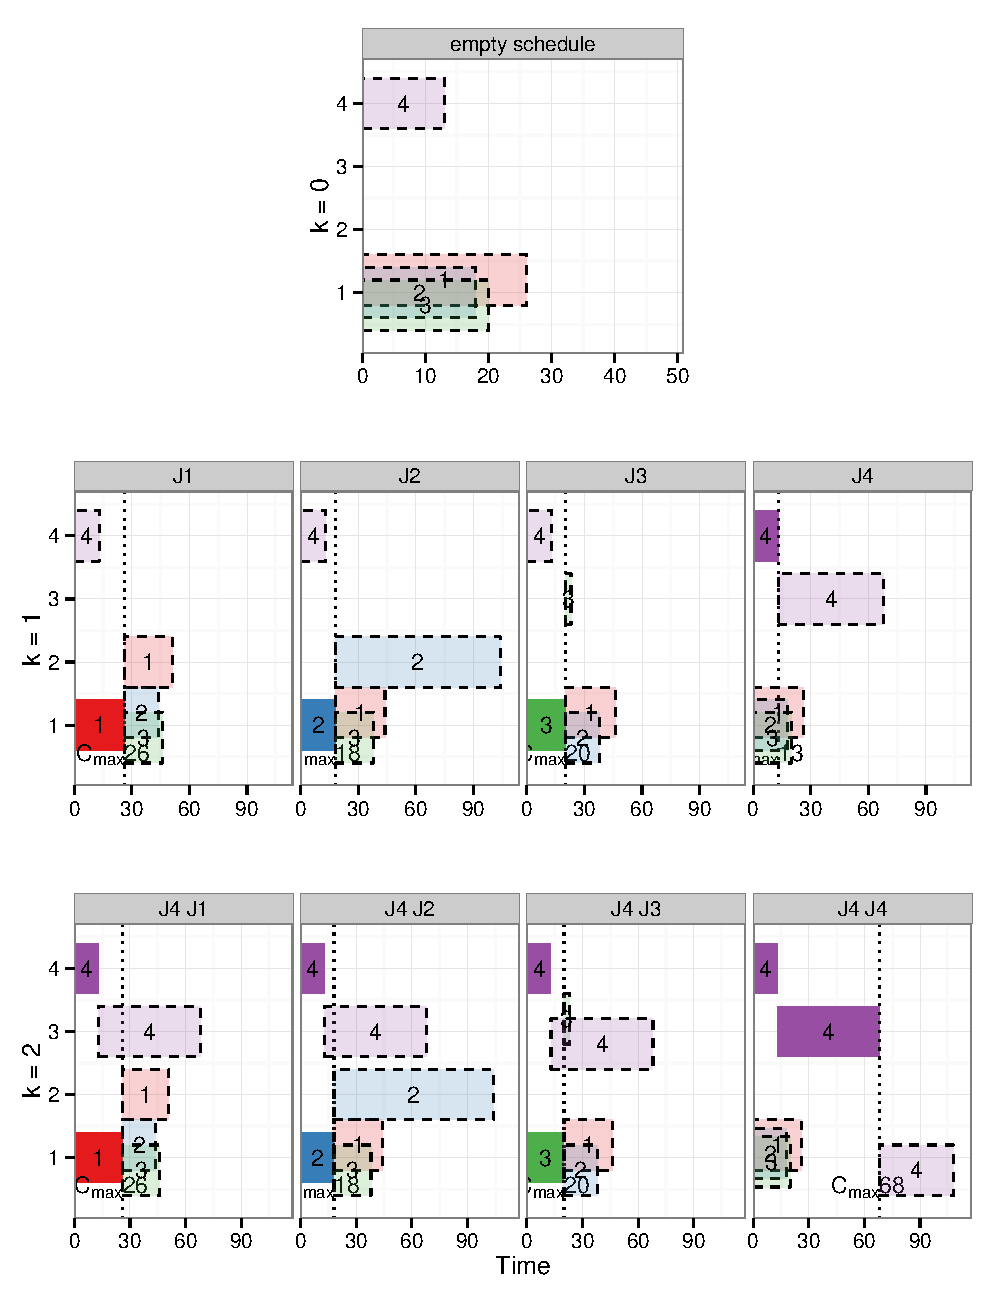
\includegraphics[width=\textwidth]{gametree}};
  \begin{scope}[x={(image.south east)},y={(image.north west)}]
  %% next four lines will help you to locate the point needed by forming a 
  %%grid. comment these four lines in the final picture.↓
  %\draw[help lines,xstep=.1,ystep=.1] (0,0) grid (1,1);
  %\draw[help lines,xstep=.05,ystep=.05] (0,0) grid (1,1);
  %\foreach \x in {0,1,...,9} { \node [anchor=north] at (\x/10,0) {0.\x}; }
  %\foreach \y in {0,1,...,9} { \node [anchor=east] at (0,\y/10) {0.\y};}
  %% upto here↑
  \node (J0) at (0.5,0.71) {};
  \node (J1) at (0.19,0.65) {};
  \node (J2) at (0.42,0.65) {};
  \node (J3) at (0.65,0.65) {};
  \node (J4) at (0.85,0.65) {};
  \draw[-latex] (J0) to[out=-20,in=+20] (J1);
  \draw[-latex] (J0) to[out=-20,in=+20] (J2);
  \draw[-latex] (J0) to[out=-20,in=+20] (J3);
  \draw[-latex] (J0) to[out=-20,in=+20] (J4);
  \node (J4) at (0.82,0.38) {};
  \node (J4J1) at (0.19,0.31) {};
  \node (J4J2) at (0.42,0.31) {};
  \node (J4J3) at (0.65,0.31) {};
  \node (J4J4) at (0.85,0.31) {};
  \draw[-latex] (J4) to[out=-20,in=+20] (J4J1);
  \draw[-latex] (J4) to[out=-20,in=+20] (J4J2);
  \draw[-latex] (J4) to[out=-20,in=+20] (J4J3);
  \draw[-latex] (J4) to[out=-20,in=+20] (J4J4);
  \end{scope}
  \end{tikzpicture}

    \vspace{-27pt}
    \caption[Partial Game Tree for \jsp]{Partial Game Tree for \jsp\ for the 
        first two dispatches. 
        Top layer depicts all possible dispatches (dashed) for an empty 
        schedule. 
        Middle layer depicts all possible dispatches given that one of the 
        dispatches from the layer above has been executed (solid). 
        Bottom layer depicts when job $J_4$ on machine $M_4$ has been chosen to 
        be dispatched from the previous layer, moreover it depicts all possible 
        next dispatches from that scenario.}
    \label{fig:example:gametree}
\end{figure}

\vspace*{-24pt}
\section{\Jsp\ tree representation}\label{sec:gen:gametree}
Continuing with the example from \cref{sec:jsp:example}, 
\cref{fig:example:gametree} shows how the first two dispatches could be 
executed for a $4\times5$ \jsp\ from \cref{sec:jsp:example}.
In the top layer one can see an empty schedule.
In the middle layer one of the possible dispatches from the layer above is 
fixed, and one can see the resulting schedule, i.e., what are the next possible 
dispatches given this scenario? Assuming $J_4$ would be dispatched first, the 
bottom layer depicts all the next possible partial schedules.

This sort of tree representation is similar to \emph{game trees} 
\citep[cf.][]{Rosen03} where the root node denotes the initial (i.e. empty) 
schedule and the leaf nodes denote the complete schedule (resulting after 
$n\cdot m$ dispatches, thus height of the tree is $K$), therefore the 
distance $k$ from an internal node to the root yields the number of operations 
already dispatched. Traversing from root to leaf node one can obtain a sequence 
of dispatches that yielded the resulting schedule, i.e., the sequence indicates 
in which order the tasks should be dispatched for that particular schedule. 

\section{Labelling schedules w.r.t. optimal decisions} 
%\label{sec:trdat:label}
One can easily see that sequence $\vchi$ from \cref{eq:vchi} for task 
assignments is by no means unique. 
Inspecting a partial schedule further along in the dispatching process such as 
in \cref{fig:example:midway}, then let's say $J_2$ would be dispatched next, 
and in the next iteration $J_4$. 
Now this sequence would yield the same schedule as if $J_4$ would have been 
dispatched first and then $J_2$ in the next iteration. 
This is due to the fact they have non-conflicting machines, which indicates 
that some of the nodes in game tree can merge. 
Meanwhile, the states of the schedule are different and thus their 
features, although they manage to yield with the same (partial) schedule at a 
later date.  % ATHUGASEMD 1 -- SEQ. REP NON-UNIQUE
In this particular instance one can not infer that choosing $J_2$ is better and 
$J_4$ is worse (or vice versa) since they can both yield the same solution.

Furthermore, in some cases there can be multiple optimal solutions to the same 
problem instance. 
Hence not only is the sequence representation `flawed' in the sense that slight 
permutations on the sequence are in fact equivalent w.r.t. the end-result.
In addition, varying permutations of the dispatching sequence (however given 
the same partial initial sequence) can result in very different complete 
schedules but can still achieve the same makespan, and thus same \fullnamerho\ 
(which is the measure under consideration). 
Care must be taken in this case that neither resulting features are labelled 
\footnote{Here the tasks labelled `optimal' do not necessarily yield the
  optimum makespan (except in the case of following expert policy $\pi_\star$), 
  instead these are the optimal dispatches for the given partial schedule.} 
as undesirable. 
Only the features from a dispatch yielding a truly suboptimal solution should 
be labelled undesirable. 

\section{Computational growth}
The creation of the game tree for \JSP\ can be done recursively for all 
possible permutations of dispatches, resulting in a full \mbox{$n$-ary} tree 
(since $|\mathcal{L}|\leq n$) of height $K$. 
Such an exhaustive search would yield at the most $n^K$ leaf nodes. Worst case 
scenario being no sub-trees merge.

\noindent Since the internal vertices (i.e. partial schedules) are only of 
interest to learn,\footnote{The root is the empty initial schedule and for the
  last dispatch there is only one option left to choose from, so there is no 
  preferred `choice' to learn.} 
the number of those can be at the most \mbox{${}^{n^K-1}/_{n-1}$}.
Even for small dimensions of $n$ and $m$ the number of internal vertices are 
quite substantial and thus too computationally expensive to investigate them 
all. Not to mention that this is done iteratively for all $N_{\train}$ 
problem instances.

Since we know that once a job is processed on all of its machines, then it 
stops being a contender for future dispatches, therefore the all possible 
assignments of operations for an $n\times m$~~\JSP\ would require an 
examination of $(n!)^m$ \citep{Giffler60}, thus a $6\times5$ problem may have 
at most $1.93\cdot10^{14}$ possible solutions, and for $10\times10$ problem 
then it's $3.96\cdot10^{65}$ solutions! Thus the factorial growth makes it 
infeasible for exploring all nodes to completion. However, our training data 
consist of relatively large $N_{\train}$, so even though we will only 
pursue one trajectory per instance, then the aggregated training data will give 
it variety.

\section{Trajectory sampling strategies}\label{sec:trdat:tracks}
For each feature in \cref{eq:Phi} we need to keep track of the resulting 
makespan for its dispatched job. 
As a result, we obtain the meta-data from 
\cref{fig:rice} as follows, 
\begin{equation}\label{eq:trdat:metadata}
\{\Phi^\pi,\mathcal{Y}^\pi\} := 
\condset{\{ \vphi^j, C_{\max}^{\pi_\star(\vchi^j)}
    \}}{J_j\in\mathcal{L}^{(k)}}_{k=1}^K \in \mathcal{F} \times \mathcal{Y}
\end{equation}
for a single problem instance $\vec{x}\in\mathcal{P}_{\train}$, and where 
$C_{\max}^{\pi_\star(\vchi^j)}$ denotes the optimal makespan (i.e. following 
the expert policy $\pi_\star$) from the resulting post-decision state $\vchi^j$.

Due to superabundant possible solutions for a single problem instance, 
there needs to be some logic based on how to sample the state-space for a 
valuable outcome. Especially considering the cost of correctly labelling 
\footnote{Optimal solutions can be obtained by using a commercial software 
    package by \citet{gurobi}, which has a free academic licence. However, GLPK 
    by \citet{glpk} has a free licence. Alas, GLPK has a lacklustre performance 
    w.r.t. speed for solving $10\times10$ \JSP.}
each dispatch that is encountered.\footnote{Generally it takes 
    only several hours to collect $N_{\train}^{6\times5}=500$. Alas, when 
    going to higher dimension, $N_{\train}^{10\times10}=300$ 
    really becomes an issue, as \jrnd{10}{10} needs a few days, and 
    \jrndn{10}{10} or \frnd{10}{10} require several weeks!}
Obviously we'd like to inspect optimal solutions as they are what we'd like to 
mimic. Moreover, since we'd like to infer the footprints in instance space for 
the SDRs we started doing in \cref{ch:defdifficulty}, then we will consider 
them also.
Similarly, the weights for \cref{eq:CDR:feat} that were optimised directly 
using from evolutionary search (cf. \cref{ch:esmodels}) will also be used.

\clearpage
To clarify, the trajectory sampling strategies for collecting a feature set and 
its corresponding labelling for \cref{eq:trdat:metadata} are the following:
\begin{description}
    \item[Optimum trajectory, \PhiSet{\OPT} or \PhiSet{\pi_\star},] at each 
    dispatch some (random) optimal task is dispatched. This is also referred to 
    following the expert policy, $\pi_\star$.
    \item[SPT trajectory, \PhiSet{\SPT},] at each dispatch the task 
    corresponding to shortest processing time is dispatched, i.e., following 
    \sdr~SPT.
    \item[LPT trajectory, \PhiSet{\LPT},] at each dispatch the task 
    corresponding to largest processing time is dispatched, i.e., following 
    \sdr~LPT.
    \item[LWR trajectory, \PhiSet{\LWR},] at each dispatch the task 
    corresponding to least work remaining is dispatched, i.e., following 
    \sdr~LWR.
    \item[MWR trajectory, \PhiSet{\MWR},] at each dispatch the task 
    corresponding to most work remaining is dispatched, i.e., following 
    \sdr~MWR.
    \item[Random trajectory, \PhiSet{\RND},] at each dispatch some random task 
    is dispatched.
    \item[CMA-ES trajectories, \PhiSet{\minRho} and \PhiSet{\minCmax},] at each 
    dispatch the task  corresponding to highest priority, computed with fixed 
    weights $\vec{w}$, which were obtained by optimising the mean for 
    \fullnamerho, with CMA-ES optimisation from \cref{ch:esmodels}. 
    \item[All trajectories, \PhiSet{\ALL},] denotes all aforementioned 
    trajectories were explored, i.e., \vspace*{-18pt}
    \begin{equation} \nonumber
    \Phi^{\ALL}:=\condset{\Phi^{A}}{\forall A \in 
    \left\{\pi_\star,\text{~SPT,~LPT,~LWR,~MWR,~RND,~}\minRho,\minCmax\right\}}
    \end{equation}
\end{description}

When following optimal trajectory, then due to the nature of the sequence 
representation (i.e. $\vchi$), the earlier stages for \Problem{j.rnd} of the 
dispatching are more or less equivalent and thus irrelevant (cf. 
\cref{fig:diff:case:OPT}). 
Hence it is appropriate to follow some random optimal path to begin with and 
then go after some (if not all possible) optimal paths until completion at step 
$K$. 

In the case of the \PhiSet{\SDR} and \PhiSet{\CMAES} trajectories it is 
sufficient to explore each trajectory exactly once for each problem instance. 
Whereas, for \PhiSet{\OPT} and \PhiSet{\RND} there can be several 
trajectories worth exploring, however, only one is chosen (at random). It is 
noted that since the number of problem instances, $N_{\train}$, is 
relatively large, it is deemed sufficient to explore one trajectory for each 
instance, in those cases as well.

These trajectory strategies were initially introduced in \cref{InRu15a}. 
However, more SDR-based trajectories are now addressed since, e.g., LWR is 
considered more favourable for \fsp\ rather than MWR (cf. 
\cref{ch:defdifficulty}). 

The number of features that were collected on a step-by-step basis for 
\Problem[6\times5]{\train} in \cref{tbl:data} is illustrated in 
\cref{fig:size:Phi:K}. 
There is an apparent stair-like structure for LWR, in accordance with its 
motivation (cf. \cref{sec:SDR}), which is completing jobs advanced in their 
progress, that is to say minimising $\mathcal{L}$ and from \cref{eq:Phi} we 
have $\abs{\Phi}\propto\abs{\mathcal{L}}$.
Whereas MWR tries to keep the jobs more balanced, hence more steady 
$\abs{\mathcal{L}}$, until at $k>(K-n)$ then \mbox{$\abs{\mathcal{L}} \lneq 
(K-k)$}, which explains the sharp decent near the end for MWR.
\Cref{tbl:size:Phi:K} gives the total size for $\abs{\Phi}$, indicating the
number of optimisations needed for obtaining $\mathcal{Y}$.

\begin{figure}[p]
    \includegraphics[width=\textwidth]{{trdat.size.6x5}.pdf}
    \vspace{-24pt}
    \caption[Size of feature set, $\abs{\Phi}$]{Size of $6\times5$ feature
    set, $\abs{\Phi}$, over different trajectory strategies}
    \label{fig:size:Phi:K}
\end{figure}

\begin{table}[p]\centering
\caption[Total number of features in $\Phi$ for all $K$ steps]{Total number of 
features in $\Phi$ for all $K$ steps. Note `--' denotes not available.}
\label{tbl:size:Phi:K}
{\setlength{\tabcolsep}{2pt} \scriptsize
\begin{tabular}{lcccccccccccc}
  \toprule 
  Track
&\multicolumn{9}{c}{\Problem[6\times5]{\train}, $N_{\train}=500$} 
&\multicolumn{3}{c}{\Problem[10\times10]{\train}, $N_{\train}=300$} 
\\
  & $j.rnd$ & $j.rndn$ & $j.rnd,J_1$& $j.rnd,M_1$ & $f.rnd$ & $f.rndn$ & 
  $f.jc$ & $f.mc$ & $f.mxc$ & $j.rnd$ & $j.rndn$ & $f.rnd$ \\ 
  \midrule
  SPT & 63197 & 63074 & 64560 & 61320 & 63287 & 63123 & 53678 & 66995 & 66216 
  & 211351 &   -- &   -- \\ 
  LPT & 63516 & 63374 & 63595 & 62864 & 63535 & 63320 & 53746 & 66356 & 65662 
  & 210490 &   -- &   -- \\ 
  LWR & 52500 & 52500 & 52500 & 52500 & 52500 & 52500 & 52500 & 52500 & 5250 
  & 165000 &   -- &   -- \\ 
  MWR & 79230 & 82500 & 78327 & 77934 & 79288 & 82500 & 80546 & 82498 & 8245 
  & 280739 &   -- &   -- \\  
  RND & 71390 & 71608 & 71445 & 71463 & 71427 & 71945 & 71558 & 71456 & 7149 
  & 252515 &   -- &   -- \\  
  OPT & 76592 & 78176 & 74109 & 74069 & 70037 & 69180 & 69716 & 71602 & 7102 
  & 272858 & 277717 & 211763 \\  
  $\minRho$ & 78443 & 81248 & 78673 & 78866 & 68986 & 55943 & 60755 & 53707& 
  74997 & 277851 & -- & -- \\ 
  $\minCmax$ & 79343 & 81226 & 77903 & 79078 & 68602 & 56789 & 54781 & 52502 & 
  52510 & 276634 & -- & -- \\ \midrule
  ALL & 564211 & 573706 &  561112 & 558094 & 537662 & 515300 & 497280 &  517616 
  & 537121 & 1947438 & 277717 & 211763 \\
  \bottomrule
\end{tabular}}
\end{table}

 %ch.5
\HeaderQuote{I don't believe there's an atom of meaning in it.}{Alice}

\chapter{Analysing Solutions}\label{ch:analysingsol} 

\FirstSentence{I}{t is interesting to know if the difference} in the structure 
of the schedule is time dependent, e.g.,  is there a clear time of divergence 
within the scheduling process? 
Moreover, investigation of how sensitive is the difference between two sets of 
features, e.g., can two schedules with similar feature values yield 
\begin{enumerate*}[itemjoin={{? }}, itemjoin*={{? Or }}, after={{? }}]
    \item completely contradictory outcomes (i.e. one poor and one good 
    schedule)
    \item will they more or less follow the their predicted trend
\end{enumerate*}
If the latter is the prevalent case, then instances need to be segregated 
w.r.t. their difficulty, where each has their own learning algorithm 
implemented, for a more meaningful overall outcome.  

Essentially this also answers the question of whether  it is in fact feasible 
to discriminate between \emph{good} and \emph{bad} schedules using the 
currently selected features as a measure for the quality of a solution. 
If results are contradictory, then it is an indicator the features selected are 
not robust enough to capture the essence of the data structure and some key 
features are missing from the feature set that could be able to discriminate 
between \emph{good} and \emph{bad} schedules. 
Additionally, there is also the question of how to define `similar'
schedules, and what measures should be used? This 
\lcnamecref{ch:defdifficulty} describes some preliminary experiments with 
the aim of investigating the feasibility of finding distinguishing features 
corresponding to \emph{good} and \emph{bad} schedules in \jsp. To summarise
\begin{enumerate*}[itemjoin={{? }}, itemjoin*={{? And }}, after={{? }}]
    \item is there a time of divergence
    \item what are `similar' schedules
    \item do similar features yield contradictory outcomes
    \item are extra features needed
    \item what can be learned from feature behaviour
\end{enumerate*}

\emph{Remark:} \Cref{fig:diff:opt:unique,fig:diff:opt:rnd} 
depict the mean over all the training data, which are quite noisy 
functions. Thus, for clarity purposes, they are fitted with local polynomial 
regression, making the boundary points sometimes biased. 
\Cref{InRu15b} depicts the raw mean as is, albeit only for $10\times10$ problem 
spaces, which is also done here for 
\cref{fig:diff:extr:SDR,fig:diff:case:OPT,fig:diff:extr:features,fig:diff:extr:SDR,fig:diff:opt:evol}.

\section{Making optimal decisions}
In order to create successful \dr, a good starting point is 
to investigate the properties of optimal solutions and hopefully be able to 
learn how to mimic such `good' behaviour. 
For this, we follow an optimal solution (cf. \PhiSet{\OPT} in 
\cref{sec:trdat:tracks}),
and inspect the evolution of its features  (defined in \cref{tbl:features}) 
throughout the dispatching process, which is detailed in \cref{ch:gentrdat}. 
Moreover, it is noted, that there are several optimal solutions available for 
each problem instance. However, it is deemed sufficient to inspect only one 
optimal trajectory per problem instance as there are $N_{\train}$ 
independent instances which gives the training data variety. 

Firstly, we can observe that on a step-by-step basis there are several optimal 
dispatches to choose from. \Cref{fig:diff:opt:unique} depicts how the number of 
optimal dispatches evolve at each dispatch iteration. Note, that only one 
optimal trajectory is pursued (chosen at random), hence this is only a lower 
bound of uniqueness of optimal solutions.
As the number of possible dispatches decrease over time, 
\cref{fig:diff:opt:rnd} 
depicts the probability of choosing an optimal dispatch at each iteration. 

To generalise, we could consider the probability of optimality as a sort of 
stepwise `training accuracy.' Then for a given policy $\pi$, we'd formalise its 
optimality (yet still maintaining optimal trajectory) as, 
\begin{equation} \label{eq:tracc:opt}
    \xi^\star_{\pi} := \Exp[\pi_{\star}]{\pi_{\star} = \pi}
\end{equation}
that is to say the mean likelihood of our policy $\pi$ being equivalent to the 
expert policy $\pi_\star$, i.e., $Y^{\pi_\star}=Y^\pi$. Note, for 
$\xi^\star_\pi$ we 
only need $\{\Phi^{\pi_\star},\mathcal{Y}^{\pi_\star}\}$ from 
\cref{eq:trdat:metadata}
\begin{enumerate*}
    \item retrace $\pi_\star$ as done in \cref{pseudo:constructJSP}
    \item inspect if the job $J_{j^*}$ chosen by $\pi$ yields the same 
    $C_{\max}^{\pi_\star(\vchi^{j^*})}$ as the true optimum, 
    $C_{\max}^{\pi_\star}$
\end{enumerate*}

\begin{figure}
  \centering
  \subcaptionbox{$6\times5$\label{fig:diff:opt:unique:6x5}}{
    \includegraphics[width=\linewidth]{figures/{stepwise.6x5.OPT.unique}.pdf}}
  \\
  \subcaptionbox{$10\times10$\label{fig:diff:opt:unique:10x10}}{
    \includegraphics[width=\linewidth]{figures/{stepwise.10x10.OPT.unique}.pdf}}
  \caption[Number of unique optimal dispatches]{Number of unique optimal 
    dispatches (lower bound).}
  \label{fig:diff:opt:unique}
\end{figure}

\begin{figure}\centering
  \subcaptionbox{$6\times5$\label{fig:diff:opt:rnd:6x5}}{
    \includegraphics[width=\linewidth]{figures/{stepwise.6x5.OPT}.pdf}}
  \\
  \subcaptionbox{$10\times10$\label{fig:diff:opt:rnd:10x10}}{
    \includegraphics[width=\linewidth]{figures/{stepwise.10x10.OPT}.pdf}}
  \caption{Probability of choosing optimal move (at random)}
  \label{fig:diff:opt:rnd}
\end{figure}

\section{Making suboptimal decisions}\label{sec:diff:opt:sub}
Looking at \cref{fig:diff:opt:rnd}, \jrnd{10}{10} has a relatively high 
probability 
($70\%$ and above) of choosing an optimal job. However, it is imperative to 
keep making optimal decisions, because once off the optimal track the 
consequences can be dire. To demonstrate this interaction, 
\cref{fig:diff:case:OPT} 
depicts the worst and best case scenario of \namerho, once you've fallen off 
the optimal track, defined as follows,
\begin{subequations}\label{eq:bwc:opt}
  \begin{eqnarray} 
  \zeta_{\min}^{\star}(k) &:=& \Exp[\pi_\star]{\given{\min(\rho)}{
      \forall C_{\max}^{\vchi^j} \gneq C_{\max}^{\pi_\star} 
      \wedge J_j\in\mathcal{L}^{(k)} }} \\
  \zeta_{\max}^{\star}(k) &:=& \Exp[\pi_\star]{\given{\max(\rho)}{
      \forall C_{\max}^{\vchi^j} \gneq C_{\max}^{\pi_\star}
      \wedge J_j\in\mathcal{L}^{(k)} }}
  \end{eqnarray}
\end{subequations}
Note, that this is given that you make \emph{one} wrong 
turn. Generally, there will be many mistakes made, and then the compound 
effects of making suboptimal decisions really start adding up. 
In fact, \cref{fig:diff:extr:SDR} shows the probability of optimality when 
following a fixed SDR (i.e. if \cref{eq:tracc:opt} is conditioned on $\pi$ 
instead of $\pi_\star$).

It is interesting that for \JSP, then making suboptimal decisions makes more of 
an impact on the resulting makespan as the dispatching process progresses. 
This is most likely due to the fact that if a suboptimal decision is made in 
the early stages, then there is space to rectify the situation with the 
subsequent dispatches. 
However, if done at a later point in time, little is to be done as the damage 
has already been inflicted upon the schedule. 
However, for \FSP, the case is the exact opposite. Under those circumstances 
it's imperative to make good decisions right from the get-go. This is due to 
the major structural differences between \jsp\ and \fsp, namely the latter 
having a homogeneous machine ordering, constricting the solution immensely. 
Luckily, this does have the added benefit of making \fsp\ less vulnerable for 
suboptimal decisions later in the decision process. 

\begin{figure}\centering
  \subcaptionbox{$6\times5$\label{fig:diff:case:OPT:6x5}}{
    \includegraphics[width=\linewidth]{figures/ALL/{stepwise.6x5.OPT.casescenario}.pdf}\vspace*{-12pt}}
  \\
  \subcaptionbox{$10\times10$\label{fig:diff:case:OPT:10x10}}{
    \includegraphics[width=\linewidth]{figures/ALL/{stepwise.10x10.OPT.casescenario}.pdf}\vspace*{-12pt}}
  \caption[Mean \namerho, for best and worst case scenario for making one 
  suboptimal move]{Mean \namerho, for best and worst case scenario of when 
  making \emph{one} suboptimal dispatch (i.e. $\zeta_{\min}^{\star}$ and 
  $\zeta_{\max}^{\star}$), depicted as lower and upper bound, 
  respectively. Moreover, mean suboptimal move is given as dashed line.}
  \label{fig:diff:case:OPT}
\end{figure}


\section{Optimality of extremal features}\label{sec:diff:opt:ext}
The training accuracy from \cref{eq:tracc:opt} of the aforementioned 
features from \cref{tbl:features}, or probability of a job chosen by an 
extremal value for a feature being able to yield an optimal makespan on a 
step-by-step basis, i.e., $\xi^\star_{\pm\phi_i}$, 
is depicted in \cref{fig:diff:extr:features}, for both \jrnd{6}{5} and 
\jrnd{10}{10}.\footnote{Additional problem spaces for $\xi^\star_{\pm\phi_i}$
    can be found in \shiny: Features $>$ Extremal.}
Moreover, the dashed line represents the benchmark of randomly guessing the 
optimum, $\xi^\star_{\RND}$ (cf. \cref{fig:diff:opt:rnd}).
Furthermore, the \lcnamecref{fig:diff:extr:features}s are annotated with the 
corresponding mean \namerho, for the training set if it were scheduled solely 
w.r.t. that extremal feature.

Generally, a high stepwise optimality means a low $\rho$, e.g., 
\phiGlobalRelated, save for \phiRNDstd.\footnote{Note, \phiRNDstd\ is 
non-informative on its own, as a tight standard deviation implies either 
consistently high \emph{or} low $C_{\max}$ from the roll-outs.} 
Unfortunately, it's not always so predictable. Take for instance \phiproc, then 
the minimum value gives a better $\rho$, even though it's unlikelier to be 
optimal than it's maximum counterpart.

\clearpage
Before inspecting the local based features further. Notice that the staggering 
performance edge for \phiRNDmin\ is lost when going to a higher dimension (cf. 
\phiRNDmin\ in \cref{fig:diff:extr:jrnd:6x5} has $\rho=1.3\%$ and increases to 
8.8\% in  \cref{fig:diff:extr:jrnd:10x10}), implying that 100 random roll-outs 
for are not sufficient for fully exploring $10\times10$ state-space, yet highly 
competitive for $6\times5$.

\begin{figure}\centering
    \captionsetup{list=no}
    \subcaptionbox{\jrnd{6}{5}\label{fig:diff:extr:jrnd:6x5}}{
        \includegraphics[width=\linewidth]{figures/{j.rnd}/{stepwise.6x5.OPT.extremal}.pdf}}
    \caption{Probability of extremal feature being optimal}
    \label{fig:diff:extr:features}
\end{figure}
\begin{figure}\centering
    \captionsetup{list=no}
    \ContinuedFloat
    \subcaptionbox{\jrnd{10}{10}\label{fig:diff:extr:jrnd:10x10}}{
        \includegraphics[width=\linewidth]{figures/{j.rnd}/{stepwise.10x10.OPT.extremal}.pdf}}
    \caption{}
    \MyCaption{Probability of extremal feature being 
    optimal}{fig:diff:extr:jrnd:6x5}{fig:diff:extr:jrnd:10x10}
\end{figure}

\begin{figure}[p]\centering
  \captionsetup{list=no}
  \subcaptionbox{$6\times5$\label{fig:diff:extr:SDR:6x5}}{
    \includegraphics[width=\linewidth]{figures/{stepwise.6x5.SDR}.pdf}}
  \caption[Probability of SDR yielding optimal move]{
    Probability of SDR yielding optimal move. 
    Both optimal (solid: $\xi^\star_{\SDR}$) and SDR-based (dashed: 
    $\xi_{\SDR}$) trajectories are inspected.}
  \label{fig:diff:extr:SDR}
\end{figure}
\begin{figure}[p]\centering
  \captionsetup{list=no}
  \ContinuedFloat
  \subcaptionbox{$10\times10$\label{fig:diff:extr:SDR:10x10}}{
    \begin{tikzpicture}
    \node[anchor=south west,inner sep=0] (image) at (0,0,0) 
    {\includegraphics[width=\linewidth]{figures/{stepwise.10x10.SDR}.pdf}};
    \begin{scope}[x={(image.south east)},y={(image.north west)}]
    \node (zoom) at (0.27,.45)
    {\includegraphics[width=0.24\linewidth]{figures/j.rnd/{stepwise.10x10.SDR.zoom}.pdf}};
    \end{scope}
    \end{tikzpicture}\vspace*{-12pt}}
  \caption{Note, due to computational complexity, only \jrnd{10}{10} has 
    SDR-based trajectories also inspected. Otherwise, only optimal is pursued.}
  \MyCaption{Probability of SDR being optimal 
    move}{fig:diff:extr:SDR:6x5}{fig:diff:extr:SDR:10x10}
\end{figure}

\subsection*{Optimality of SDRs}
Let's limit ourselves to only features that correspond to SDRs from 
\cref{sec:SDR}. Namely, \cref{eq:CDR:SDR} yield
\begin{enumerate*}
    \item \phiproc\ for SPT and LPT
    \item \phijobWrm\ for LWR and MWR 
\end{enumerate*}
By choosing the lowest value for the first SDR, and highest value for the 
latter SDR, i.e., the extremal values for those given features. 
\Cref{fig:diff:extr:SDR} depicts the corresponding probabilities from 
\cref{fig:diff:extr:features} in one graph, for all problem spaces in 
\cref{tbl:data}.

Now, let's bare in mind \namerho, of applying SDRs throughout the dispatching 
process (cf. box-plots of which in \cref{fig:SDR:boxplot}), then there is a 
some correspondence between high probability of stepwise optimality and low 
$\rho$. Alas, this isn't always the case, for \jrnd{10}{10} 
$\xi^\star_{\SPT}$ always outperforms $\xi^\star_{\LPT}$ in 
choosing a 
dispatch which may result in an optimal schedule. However, this does not 
transcend to SPT having a lower $\rho$ value than LPT. Hence, it's not enough 
to just learn optimal behaviour, one needs to investigate what happens once we 
encounter suboptimal state spaces.

Since we know that our SDR heuristics aren't  perfect, and they're bound 
to make mistakes at some point. 
It's interesting to see how that stepwise optimality evolves for its intended 
trajectory, thereby updating \cref{eq:tracc:opt} to
\begin{equation} \label{eq:tracc:track}
    \xi_{\pi} := \Exp[\pi]{\pi_{\star} = \pi}
\end{equation}
\Cref{fig:diff:extr:SDR} shows the difference between $\xi^\star_{\SDR}$ and 
$\xi_{\SDR}$.
Similarly for \cref{eq:bwc:opt}, 
\begin{subequations}\label{eq:bwc:track}
\begin{IEEEeqnarray}{rCl}
  \zeta_{\min}^{\pi}(k) &:=& \Exp[\pi]{\given{\min(\rho)}{
      \forall C_{\max}^{\pi_\star(\vchi^{j})} \neq 
      C_{\max}^{\pi_\star(\vchi^{j^*})} \wedge j^* = 
      \argmax_{J_j\in\mathcal{L}^{(k)}}\{\pi(\vphi^j)\}
      }} \\
  \zeta_{\max}^{\pi}(k) &:=& \Exp[\pi]{\given{\max(\rho)}{
      \forall C_{\max}^{\pi_\star(\vchi^j)} \neq 
      C_{\max}^{\pi_\star(\vchi^{j^*})} \wedge j^* = 
      \argmax_{J_j\in\mathcal{L}^{(k)}}\{\pi(\vphi^j)\} 
      }} \\
  \zeta_{\mu}^{\pi}(k) &:=& \Exp[\pi]{\given{\rho}{
          C_{\max}^{\pi_\star(\vchi^{j^*})} \wedge j^* = 
          \argmax_{J_j\in\mathcal{L}^{(k)}}\{\pi(\vphi^j)\} 
      }} \label{eq:bwc:track:mu}
\end{IEEEeqnarray}
\end{subequations}
with the additional metric $\zeta_{\mu}^{\pi}$, which gives the mean evolution 
for \namerho, when following a fixed policy $\pi$.
Note, $\zeta^{\pi_{\star}}_{\min}=\zeta^{\star}_{\min}, 
\zeta^{\pi_{\star}}_{\max}=\zeta^{\star}_{\max}$ and 
$\zeta^{\pi_{\star}}_{\mu}=0$.
\Cref{fig:diff:case:SDR} depicts \cref{eq:bwc:track} for expert policy 
$\pi_\star$ and SDRs.

\begin{figure}[p]\centering
    \captionsetup{list=no}
    \subcaptionbox{$10\times10$\label{fig:diff:case:SDR:10x10}}{
        \includegraphics[width=0.8\linewidth]{figures/{j.rnd}/{stepwise.10x10.ALL.casescenario}.pdf}\vspace*{-12pt}}
    \caption{Mean \namerho, for best and worst case scenario when not
        following a fixed policy $\pi$ (i.e. $\zeta_{\min}^\pi$ and 
        $\zeta_{\max}^\pi$), depicted as lower and upper bound, respectively. 
        Moreover, mean evolution of $\rho$ for $\pi$ (i.e. $\zeta_{\mu}^{\pi}$) 
        is given as a dashed line.}
\end{figure}
\begin{figure}[p]\centering
    \captionsetup{list=no}
    \ContinuedFloat
    \subcaptionbox{$6\times5$\label{fig:diff:case:SDR:6x5}}{
        \includegraphics[width=\linewidth]{figures/ALL/{stepwise.6x5.ALL.casescenario}.pdf}}
    \caption{Note, $\{\zeta^{\pi^\star}_{\min},\zeta^{\pi^\star}_{\max}\}$ are 
    illustrated jointly for \Problem{\train} in \cref{fig:diff:case:OPT}}
    \MyCaption{Mean \namerho, for best and worst case scenario for not following
    a fixed policy}{fig:diff:case:SDR:10x10}{fig:diff:case:SDR:6x5}
    \label{fig:diff:case:SDR}
\end{figure}

\clearpage

A means of interpreting \cref{eq:bwc:track}, is that given a fixed policy 
$\pi$, then $\zeta_{\min}^{\pi}$ describes the potential improvement (iff 
$\zeta_{\min}^{\pi}<\zeta_{\mu}^{\pi}$) for changing the policy. Whereas, 
$\zeta_{\max}^{\pi}$ indicates the disadvantages of changing course. 
When $\zeta_{\min}^{\pi}>\zeta_{\mu}^{\pi}$, then clearly $\pi$ is not a good 
policy for said problem space, e.g., for the final dispatches of 
$\zeta_{\mu}^{\SPT}$ for \jrndJ{6}{5} or \jrnd{10}{10}. 

\emph{Remark}: \cref{eq:tracc:track,eq:bwc:track} are based on corresponding 
meta-data, $\{\Phi^\pi,\mathcal{Y}^\pi\}$ , from \cref{eq:trdat:metadata}, 
whereas \cref{eq:tracc:opt,eq:bwc:opt} reuse the same expert meta-data,
$\{\Phi^{\pi_\star},\mathcal{Y}^{\pi_\star}\}$.

\section{Simple blended dispatching rule}\label{sec:diff:opt:bdr}
The goal of this \lcnamecref{ch:defdifficulty} is to utilise feature behaviour 
to motivate new (and \emph{hopefully} better) \dr s. 
A na\"ive approach would be creating a simple blended \dr\ (BDR) which 
would be for instance switching between two SDRs at a predetermined time point. 

For instance, MWR and SPT hardly ever coincide for easy or hard schedules (cf. 
\cref{tbl:easy:cnt:10x10,tbl:hard:cnt:10x10}), so its reasonable to believe 
they could complement one another.
Going back to \cref{fig:diff:extr:SDR:10x10} a presumably good BDR for 
\jrnd{10}{10}  would be starting with $\xi^\star_{\SPT}(k)$ and then 
switching over to $\xi^\star_{\MWR}(k)$ at around time step $k=40$, where 
the SDRs change places in outperforming one another.
In addition, we can see that even though $\xi_{\SPT}(k)$ is generally 
more likely to find optimal dispatches in the initial steps, shortly after 
$k=15$ then $\xi_{\MWR}(k)$ becomes a contender again. 
A box-plot of \namerho, for \Problem[10\times10]{\train} is 
depicted in \cref{fig:diff:boxplot:BDR} for a switch between SPT to MWR at time 
steps $k=\{10,15,20,30,40\}$. Main statistics are given in \cref{tbl:BDR:stats}.

This little manipulation between SDRs does outperform SPT immensely, yet 
doesn't manage to gain the performance edge of MWR. 
This gives us insight that for \jsp, the attribute based on MWR is quite 
fruitful for good dispatches, whereas the same cannot be said about SPT -- a 
more sophisticated DR is needed to improve upon MWR. 

A reason for this lack of performance of our proposed BDR at $k=40$ is perhaps 
that by starting out with SPT in the beginning, it sets up the schedules in 
such a way that it's quite greedy and only takes into consideration jobs with 
shortest immediate processing times. 
Now, even though it is possible to find optimal schedules from this scenario, 
as \cref{fig:diff:extr:SDR} shows, the inherent structure is already taking 
place, and might make it hard to come across optimal moves by simple methods. 
Therefore it's by no means guaranteed that by simply swapping over to MWR will 
handle the situation that applying SPT has already created. 
\Cref{fig:diff:boxplot:BDR} does however show, that by applying MWR instead of 
SPT in the latter stages, does help the schedule to be more compact w.r.t. SPT. 
However, the fact remains that the schedules have diverged too far from what 
MWR would have been able to achieve on its own, i.e., using SPT downgrades the 
performance of MWR. 

Changing to MWR at $k\leq20$ is not statically significant from MWR (boost in 
mean $\rho$ is at most 0.5\%). 
However, after $k>20$ then the BDR starts diverging from MWR. 
But as pointed in \cref{sec:diff:opt:sub}, it's not so fatal to make bad moves 
in the very first dispatches for \jrnd{10}{10}, hence little is gained with 
improved classification accuracy in that region. 
But this does tell us that $\xi_\pi$ is a more reliable indicator than 
$\xi^\star_\pi$ when it comes to choosing appropriate model parameters. 
Alas, $\xi_\pi$ requires collecting the meta-data 
$\{\Phi^\pi,\mathcal{Y}^\pi\}$ from \cref{eq:trdat:metadata} for its policy 
$\pi$, whereas $\xi^\star_\pi$ reuses 
$\{\Phi^{\pi_\star},\mathcal{Y}^{\pi_\star}\}$ 
for each new policy $\pi$.

Revisiting \cref{fig:diff:case:SDR:10x10}, then we see 
$\zeta_{\mu}^{\SPT}(40)$ has already surpassed 
$\zeta_{\mu}^{\MWR}(K)$ and there are 60 operations left to dispatch. So 
a switch for BDR at $k=40$ never had a chance of improvement. 
However, at $k\leq15$ then $\zeta_{\mu}^{\SPT}(k) < 
\zeta_{\mu}^{\MWR}(k)$, which were appropriate turning points for BDR 
(although not statistically significant).

Preferably the blended dispatching rule should use best of both worlds, and 
outperform all of its inherited DRs, otherwise it goes without saying, one 
would simply keep on still using the original DR that achieved the best results.

\begin{figure}[p]
  \centering
  \includegraphics[width=\linewidth]{figures/{j.rnd}/{boxplotRho.BDR.10x10}.pdf}
  \vspace*{-24pt}
  \caption{Box plot of \jrnd{10}{10} \namerho, for BDR where SPT is applied for 
  the first 10\%, 15\%, 20\%, 30\% or 40\% of the dispatches, followed by MWR.}
  \label{fig:diff:boxplot:BDR}
\end{figure}

\begin{table}[b]
\caption{Main statistics for \jrnd{10}{10} \namerho, using BDR that changes 
from SDR at a fixed time step $k$.}\label{tbl:BDR:stats} 
\centering
\begin{tabular}{ccrlrrrrrr}
  \toprule
  SDR \#1 & SDR \#2 & $k$ & Set & Min. & 1st Qu. & Median & Mean & 
    3rd Qu. & Max. \\ \midrule
  SPT & -- & $K$ & train & 20.38 & 41.15 & 50.70 & 51.31 & 59.18 & 94.20 \\ 
  SPT & -- & $K$ & test & 22.75 & 41.39 & 49.53 & 50.52 & 58.60 & 93.03 \\ 
  MWR & -- & $K$ & train & \textbf{4.42} & \textbf{17.84} & \textbf{21.74} & 
  22.13 & 26.00 & 47.78 \\ 
  MWR & -- & $K$ & test & \textbf{3.37} & \textbf{17.07} & 21.39 & 21.65 & 
  25.98 & \textbf{41.80} \\ 
  SPT & MWR & 10 & train & 5.54 & 17.98 & 21.75 & \textbf{21.99} & 
  \textbf{25.43} & \textbf{44.02} \\ 
  SPT & MWR & 10 & test & 5.87 & 17.29 & \textbf{20.78} & \textbf{21.28} & 
  \textbf{24.67} & 44.47 \\ 
  SPT & MWR & 15 & train & 4.76 & 18.24 & 22.04 & 22.49 & 26.65 & 49.86 \\ 
  SPT & MWR & 15 & test & 7.42 & 17.60 & 21.38 & 21.83 & 25.45 & 45.98 \\ 
  SPT & MWR & 20 & train & 5.76 & 18.98 & 22.46 & 23.01 & 26.97 & 41.59 \\ 
  SPT & MWR & 20 & test & 8.31 & 18.64 & 22.92 & 23.29 & 27.10 & 49.93 \\ 
  SPT & MWR & 30 & train & 9.77 & 20.89 & 25.60 & 25.76 & 30.01 & 50.94 \\ 
  SPT & MWR & 30 & test & 4.39 & 21.20 & 26.08 & 26.25 & 30.58 & 49.88 \\ 
  SPT & MWR & 40 & train & 13.04 & 23.42 & 28.12 & 28.94 & 33.67 & 54.98 \\ 
  SPT & MWR & 40 & test & 8.55 & 24.20 & 28.16 & 28.98 & 33.20 & 57.21 \\ 
  \bottomrule
\end{tabular}
\end{table}

\section{Feature evolution}\label{sec:diff:opt:evol}
In order to put the extremal features from \cref{fig:diff:extr:features} into 
perspective, it's worth comparing them with how the evolution of the features 
are over time, depicted in \cref{fig:diff:opt:evol} for \jrnd{6}{5} and 
\jrnd{10}{10}.\footnote{Additional problem spaces can be found in \shiny: 
    Features $>$ Evolution.} 
Note that the optimal trajectory describes  how `good' features should aspire 
to be like.
We can also notice that the relative ranking in \phiGlobalRelated\ is 
proportional their expected mean \namerho\ (i.e. $\zeta_{\mu}^{\pi}(K)$). 
Although $(K-k)$-step lookahead give consistently the best (single) indicators 
for finding good solutions. 
Sadly, they are not practical features for high dimensional data due to 
computational cost. 

\begin{figure}\centering
  \captionsetup{list=no}
  \subcaptionbox{\jrnd{6}{5}\label{fig:diff:evol:jrnd:6x5}}{
    \includegraphics[width=\linewidth]{figures/{j.rnd}/{stepwise.6x5.evolution}.pdf}}
  \caption{Mean stepwise evolution of $\tilde{\vphi}$, which is scaled 
  according to \cref{eq:scale}}
  \label{fig:diff:opt:evol}
\end{figure}
\begin{figure}\centering
  \captionsetup{list=no}
  \ContinuedFloat
  \subcaptionbox{\jrnd{10}{10}\label{fig:diff:evol:jrnd:10x10}}{
    \includegraphics[width=\linewidth]{figures/{j.rnd}/{stepwise.10x10.evolution}.pdf}}
  \caption{}
  \MyCaption{Mean stepwise evolution of 
  $\tilde{\vphi}$}{fig:diff:evol:jrnd:6x5}{fig:diff:evol:jrnd:10x10}
\end{figure}

\clearpage
\section{Emergence of problem difficulty}\label{sec:diff:stepwise}

% Katie orðar: A correlation analysis between the feature space and the 
%performance space was conducted across all 1,500 problem instances revealed 
%that instance features that appear to correlate (linearly) with heuristic 
%performance are $phi(?)$ (correlation $=-0.59$) and $phi(?)$ (correlation 
%$=0.44$). None of the other instance features appear to have a linear 
%relationship with algorithmic performance.

The main focus now is on knowing \emph{when} during the scheduling process easy 
and hard problems diverge, this will be done using \PhiSet{\ALL} and 
\PhiSet{\SDR} (conditioned on the followed trajectory) for 
\jrnd{6}{5}.\footnote{Additional problem spaces can be
    found in \shiny: Footprints $>$ Stepwise.}
Individual \PhiSet{\SDR} are segregated w.r.t. its own quartiles defined 
in \cref{eq:easy.vs.hard}, whereas \PhiSet{\ALL} is using the joint quartiles 
given in \cref{tbl:easyhard:quartile:6x5}. 
Note, if a joint quartile is used for \PhiSet{\SDR}, then the segregation 
becomes highly unbalanced, e.g., for MWR the bulk is considered `easy' and 
there is only a single `hard' problem instance, as a result there 
can be no comparison between the two. 
The number of segregated problem instances for given in 
\cref{tbl:jrnd:feat:cnt}.

Rather than visualising high-dimensional data projected onto two dimensional 
space (as was the focus in \cite{SmithMilesLion5} with SOM), 
instead appropriate statistical tests with a significance level $\alpha=0.05$ 
is applied to determine if there is any difference between different data 
distributions. 
For this the two-sample Kolmogorov–Smirnov test (K-S test) is used to determine 
whether two underlying one-dimensional probability distributions differ. 
Furthermore, in order to find defining characteristics for easy or hard 
problems, a (linear) correlation is computed between features to the resulting 
\namerho\ and use a $t$-test for testing the population correlation 
coefficient. 

When inspecting any statistical difference between data distribution of 
the features on a step-by-step basis, the features at step $k+1$ are of course 
dependant on all previous $k$ steps. This results in repetitive statistical 
testing, therefore a Bonferroni correction is used to counteract the multiple 
comparisons, i.e., each stepwise comparison has the significant level
\begin{equation}
\alpha_k=\frac{\alpha}{K}
\end{equation} 
thus maintaining the $\sum_{k=1}^K\alpha_k=\alpha$ significance level. 
However, with our limited sample size both $\alpha$ and $\alpha_k$ significance 
levels are reported, where entries with Bonferroni correction are especially 
highlighted.

{\setlength{\tabcolsep}{3pt} 
\begin{table}\centering
    \caption{Number of problem instances after segregating \jrnd{6}{5} w.r.t. 
    difficulty and trajectory.}
    \label{tbl:jrnd:feat:cnt}
    \subcaptionbox{Used in \cref{fig:jrnd:feat:KStest}
        \label{tbl:jrnd:feat:cnt:KS}
        }{
        \begin{tabular}{lrrr}
            \toprule
            Track & $\#$Easy & $\#$Hard & $\#$Significant \\ 
            \midrule
            LPT & 126 & 125 & 111 \\ 
            LWR & 125 & 126 & 73 \\ 
            MWR & 125 & 125 & 150 \\ 
            SPT & 127 & 126 & 93 \\ 
            \midrule
            $\Sigma$ & 503 & 502 & 427 \\ 
            \bottomrule
        \end{tabular}
    }\quad\quad
    \subcaptionbox{Used in \cref{fig:jrnd:feat:corr}
        \label{tbl:jrnd:feat:cnt:corr}}{
        \begin{tabular}{lrr}
            \toprule
            & \multicolumn{2}{c}{$\#$Significant} \\
            Track & Easy & Hard \\ 
            \midrule
            LPT & 81 & 63 \\ 
            LWR & 121 & 48 \\ 
            MWR & 44 & 69 \\ 
            SPT & 79 & 77 \\ 
            ALL & 380 & 228 \\
            \midrule
            $\Sigma$ & 705 & 485 \\
            \bottomrule
        \end{tabular}}
\end{table}}

\begin{figure}[t]
    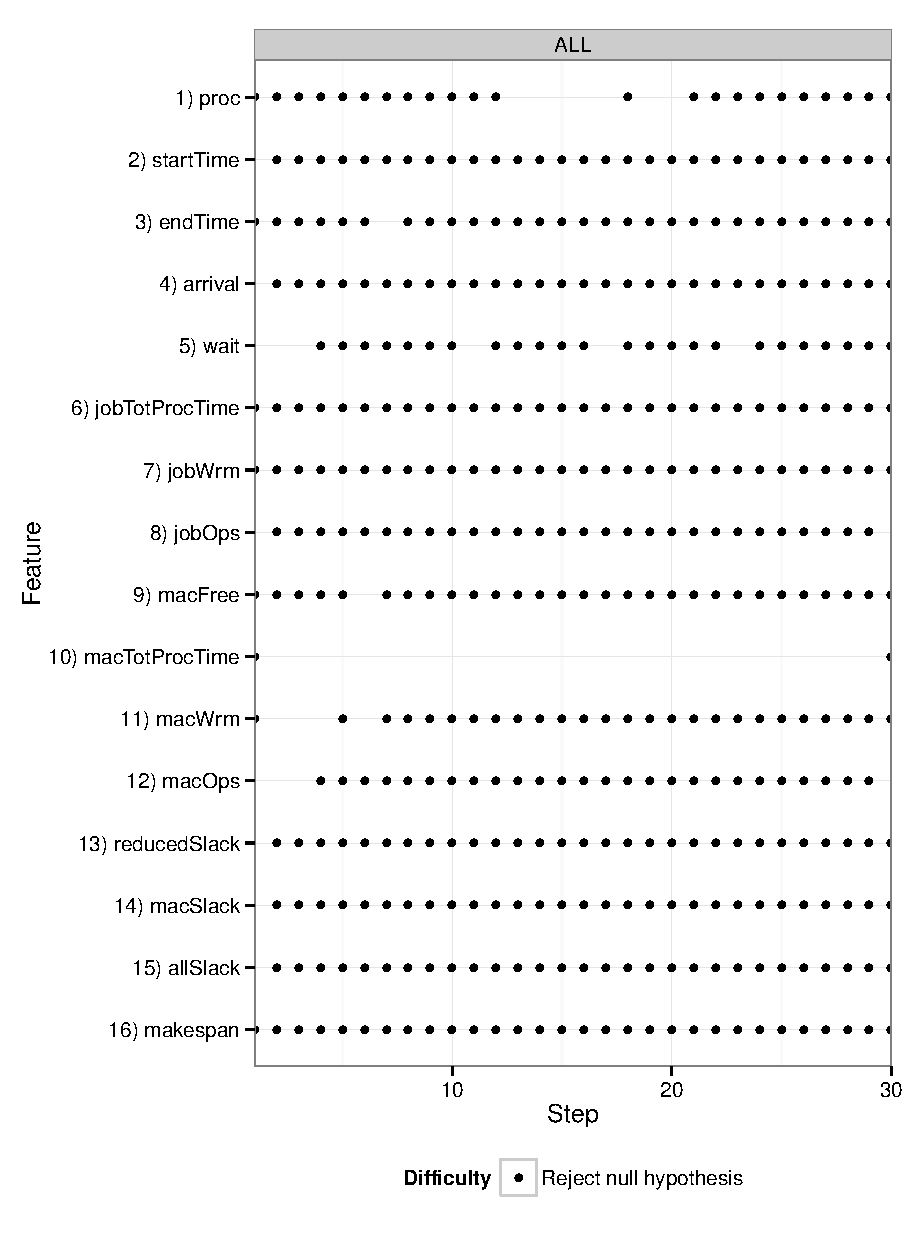
\includegraphics[width=\linewidth]{{j.rnd/phi.ks.SDR.6x5}.pdf}
    \caption{Stepwise K-S Test for features $\vphi$ segregated w.r.t. easy and 
        hard problems are drawn from the same continuous data distribution.}
    \label{fig:jrnd:feat:KStest}
\end{figure}

\begin{figure}
    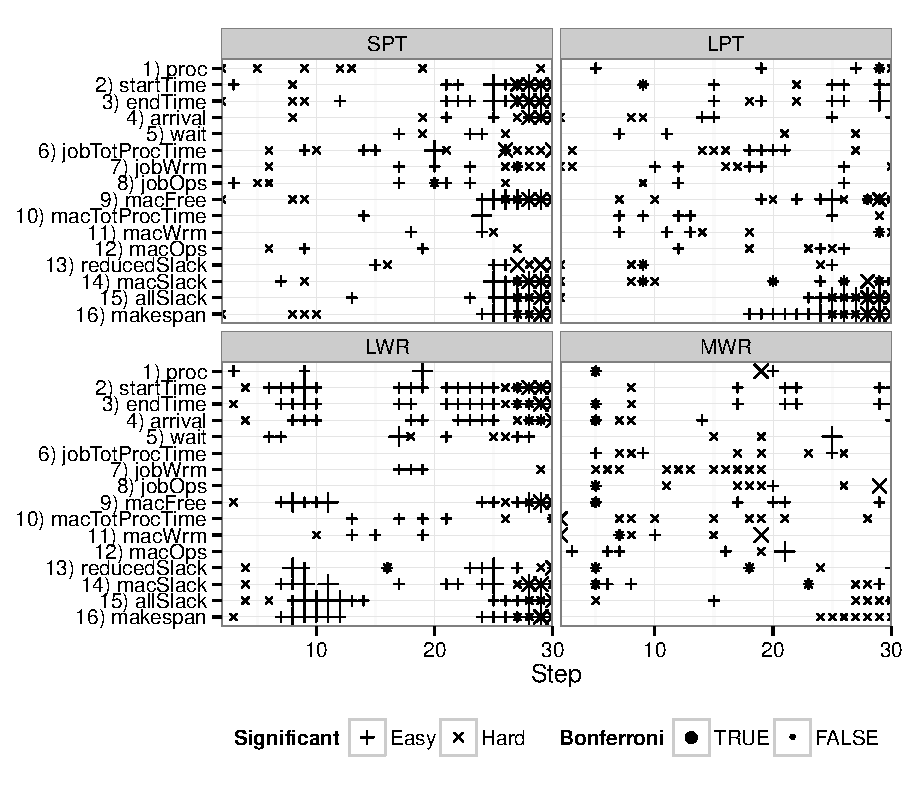
\includegraphics[width=\linewidth]{{j.rnd/phi.corr.SDR.6x5}.pdf}
    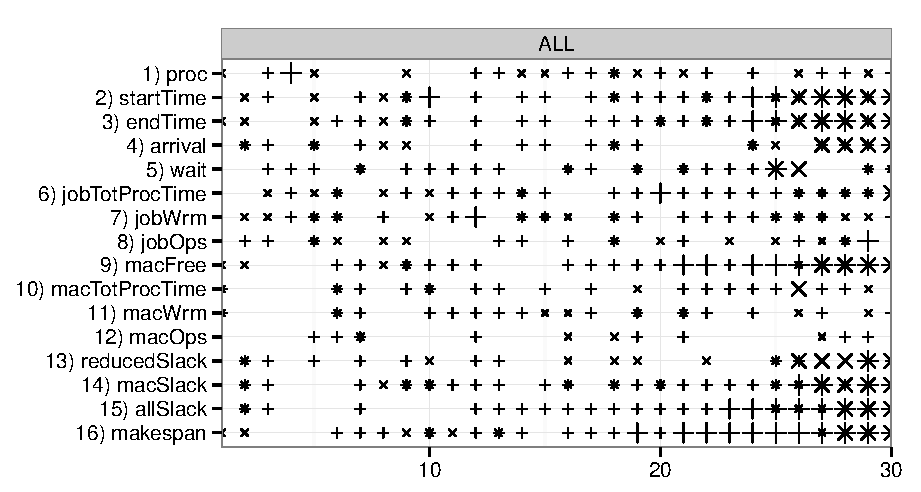
\includegraphics[width=\linewidth]{{j.rnd/phi.corr.ALL.6x5}.pdf}
    \caption{Stepwise significance of a correlation coefficient for \jrnd{6}{5} 
        features $\vphi$, segregated w.r.t. easy and hard problems, with 
        resulting \namerho.}
    \label{fig:jrnd:feat:corr}
\end{figure}

\Cref{fig:jrnd:feat:KStest} indicates the timesteps when easy and hard feature 
distributions differ. Number of problem instances of segregated sets are given 
in \cref{tbl:jrnd:feat:cnt:KS}. 
In the initial stages, the features are more or less the same. 
However, there is a clear time of divergence (many of which rejected with 
Bonferroni correction) towards the end of the scheduling process
\begin{enumerate*}
    \item around the half way mark for MWR
    \item $k=20$ for LPT
    \item around $k=25$ for SPT and LWR
\end{enumerate*}
Knowing this time of divergence, we could inspect the features from that time 
step onwards and check if they belong to our set of pre-classified `easy' 
features. If not then it could be appropriate to choose jobs that do not 
correspond that particular SDR, that is to say if \cref{fig:diff:case:SDR:6x5} 
indicates that on average $\{\zeta_{\min}^{\SDR}(k),\zeta_{\max}^{\SDR}(k)\}$ 
are performing better than if we'd continue with our intended trajectory (i.e. 
$\zeta_{\mu}^{\SDR}(k)$). This applies especially for SPT and LPT.

Unfortunately, this information comes a little to late too be of much use for 
all SDR save for MWR, as $\zeta_{\mu}^{\SDR}(k)$ is quite high for 
$SDR=\{\SPT,\LPT\}$, and for LWR nothing can be done as there is no option of 
dispatching any other job than the single one remaining (cf. e.g. 
\cref{fig:diff:evol:jrnd:6x5}).

Furthermore, \cref{fig:jrnd:feat:corr} shows when easy or hard features 
are significantly correlated to the \namerho.
There we can see an apparent difference in correlation between individual 
features with the resulting schedule depending in what stage it is in the 
scheduling process, implying that their influence varies over the dispatching 
sequencing. 

There are some common features for both difficulties considered which define 
\jsp\ on a whole. However, the significant features are quite different across 
the two difficulties, implying there is a clear difference in their data 
structure. 
The amount of significant features were considerably more for easy 
problems, indicating their key elements had been found. However, the features 
distinguishing hard problems were scarce. Most likely due to their more complex 
data structure their key features are of a more composite nature. As a result, 
new `global' roll-out features were introduced in \cref{tbl:features}. 

What is surprising is that when looking at \cref{fig:jrnd:feat:corr} then the 
active feature for the used SDR (i.e. \phiproc\ for SPT \& LPT and \phijobWrm\ 
for LWR  \& MWR) then they are hardly ever significantly correlated to final 
$\rho$.
However, their usage effects other features that are a key indicator throughout 
the dispatching process. Therefore we would need to take into account the joint 
interaction of features, and not look at them on their own as we do now. 

Take for instance \phijobWrm, which we know is a good indicator (i.e. MWR) and 
use \phiendTime\ as well, then it's possible to obtain a model (cf. 
\cref{ch:featselect}) that boosts MWR in performance by $\Delta\rho=10\%$.

Note, even though some feature are hardly ever correlated w.r.t. $\rho$, then 
that does not necessarily imply that they're a bad attribute.
Take for instance \phijobOps, which is a discrete simplification of 
\phijobWrm, whose purpose was to complete advanced jobs (i.e LWR) or 
balance progress for all jobs (i.e. MWR). 
In the case of \jrnd{6}{5} then -\phijobOps yields mean $\rho=18\%$, whereas 
it's more sophisticated counterpart, +\phijobWrm\ has a slightly lower mean 
$\rho=16$ (cf. \cref{fig:diff:extr:jrnd:6x5}).

It is possible for a \JSP\ schedule to have more than one sequential 
dispatching representation. It is especially w.r.t. the initial dispatches. 
Revisiting \cref{fig:example:midway}, if we were to dispatch $J_2$ f
first and then $J_4$, then that would be the same equivalent
temporal schedule if we did it the other way around. 
This is because they don't create a conflict for one another 
(as is the case for jobs $J_2$ and $J_3$). 
This drawback of non-uniqueness of sequential dispatching representation 
explains why there is hardly any significant difference between the 
difficulties for the initial steps of the scheduling process (cf. 
\cref{fig:jrnd:feat:KStest}).
As we can see from \cref{tbl:jrnd:feat:cnt}, the number of problem instances 
used for statistical testing is quite limited when applying on a single 
algorithm. 
Using the non-uniqueness of $\vchi$ to our advantage, where there are many jobs 
that have non-conflicting machines, thereby making subsequent dispatches 
equivalent to the previous one, i.e., $\vchi^k \approx  \vchi^{(k\pm1)}$. 
Therefore it's reasonable, when labelled optimal data is scarce, to inspect the 
stepwise statistical testing based on sliding window of the preceding and 
subsequent step, i.e., test at time $k$ is based on: 
\begin{equation}
\vphi_i^{(k)} := \condset{\phi_i^{k'}}{\forall \phi_i\in\Phi}_{k'=k-1}^{k+1} 
\end{equation}
for all individual local features $\phi_i\in\{1,\ldots,\NrFeatLocal\}$ from 
\cref{tbl:features}.

\section{Conclusions}

\todoWrite{From \cref{sec:diff:opt:ext} we noticed that high stepwise 
optimality generally implies low \namerho. Moreover, there is clearly an 
important factor \emph{when} suboptimal moves are made, as 
\cref{sec:diff:opt:sub} showed. Therefore it's not 
    }

The main objective of this \lcnamecref{ch:analysingsol} was to illustrate the 
interaction of a specific algorithm on a given problem structure and its 
properties. 
This can be considered as finding the footprint from \sdr s introduced in 
\cref{sec:SDR} on those problem spaces. 
Presumably, we could use that information to infer the complexity of our 
synthesised problem spaces summarised in \cref{tbl:data}.

\Cref{sec:diff:stepwise} showed that the emergence of a problem instances 
difficulty w.r.t. its algorithm was not noticeable until the very end of the 
dispatching process. Preferably we'd like to know this information sooner, in 
order to steer the algorithm towards a more promising state space where the 
features are `known' to have better performance. 

Since feature selection is of paramount importance in order for algorithms to 
become successful, one needs to give great thought to how features are 
selected. What kind of features yield \emph{bad} schedules? And can they be 
steered onto the path of more promising feature characteristics? This sort of 
investigation can be an indicator how to create meaningful problem generators. 
On the account that real-world problem instances are scarce, their hidden 
properties need be drawn forth in order to generate artificial problem 
instances from the same data distribution. 

The feature attributes need to be based on statistical or theoretical grounds. 
Scrutiny in understanding the nature of problem instances therefore becomes of 
paramount importance in feature engineering for learning, as it yields feedback 
into what features are important to devote more attention to, i.e., features 
that result in a failing algorithm. 

\todoWrite{Conclusions for stepwise optimality and best/worst case scenario}

In general, this sort of analysis can undoubtedly be used in better 
algorithm design which is more equipped to deal with varying problem instances 
and tailor to individual problem instance's needs, i.e., a footprint-oriented 
algorithm.


 %ch.6
\HeaderQuote{Oh my ears and whiskers, how late it's getting!}{Rabbit} 

\chapter{Preference Learning}\label{ch:prefmodels} 
\FirstSentence{L}{earning models considered in this } dissertation are based on ordinal regression in which the learning task is formulated as learning preferences. In the case of scheduling, learning which operations are preferred to others. Ordinal regression has been previously presented in \cite{Ru06:PPSN}, and given in \cref{ch:ordinal} for completeness. 

\section{Ordinal regression for \jsp}
Using the training set $\{\Phi^\pi,\mathcal{Y}^\pi\}$, given in 
\cref{eq:trdat:metadata} by following some policy $\pi$, 
let $\vphi_{o}\in\Phi^\pi$ denote the post-decision state when dispatching 
job $J_o$ corresponds to an optimal schedule being built. All post-decisions 
states corresponding to suboptimal dispatches, $J_s$, are denoted by 
$\vphi_{s}\in\Phi^\pi$. 

Let's label feature sets which were considered optimal, 
$\vec{z}_{o}=\vphi_{o}-\vphi_{s}$, and suboptimal, 
$\vec{z}_{s}=\vphi_{s}-\vphi_{o}$ by $y_o=+1$ and $y_s=-1$ respectively. 
The preference learning problem is specified by a set of preference pairs,
\begin{equation}\label{eq:Psi:jsp}
	\Psi := \bigcup_{\{\vec{x}_i\}_{i=1}^{N_{\train}}}
    \condset{
        \left\{\vec{z}_o,+1\right\},\left\{\vec{z}_s,-1\right\}}{\forall 
        (J_o,J_s) 
        \in \mathcal{O}^{(k)} \times \mathcal{S}^{(k)}}_{k=1}^K 
    \subset \Phi\times Y 
\end{equation}
where 
\begin{enumerate*}
  \item $\Phi\subset\mathcal{F}$ is the training set of $d=\NrFeatLocal$ 
  features (cf. the local features from \cref{tbl:features}) 
  \item $Y=\{-1,+1\}$ is the outcome space
  \item at each dispatch $k\in\{1,\ldots,K\}$
  \item $J_o\in\mathcal{O}^{(k)},~J_s\in \mathcal{S}^{(k)}$
  are optimal and suboptimal dispatches, respectively
\end{enumerate*}

A negative example is only created as long as $J_s$ actually 
results in a worse makespan, i.e., $C_{\max}^{\pi_\star(\vchi^s)} \gneq 
C_{\max}^{\pi_\star(\vchi^o)}$, since there can exist situations in which more 
than one operation can be considered optimal. 
Hence, $\mathcal{O}^{(k)}\cup\mathcal{S}^{(k)}=\mathcal{L}^{(k)}$, and 
$\mathcal{O}^{(k)}\cap\mathcal{S}^{(k)}=\emptyset$.
If the makespan would be unaltered, the pair is omitted from $\Psi$, since they 
give the same optimal makespan. 
This way, only features from a dispatch resulting in a suboptimal solution is 
labelled undesirable.
The approach taken here is to verify analytically, at each time step, by 
retaining the current temporal schedule as an initial state, whether it can 
indeed \emph{somehow} yield an optimal schedule by manipulating the remainder 
of the sequence, i.e., $C_{\max}^{\pi_\star(\vchi^j)}$ for all 
$J_j\in\mathcal{L}^{(k)}$. 
This also takes care of the scenario that having dispatched a job resulting in 
a different temporal makespan would have resulted in the same final makespan if 
another optimal dispatching sequence would have been chosen. 
That is to say the data generation takes into consideration when there are 
multiple optimal solutions to the same problem instance. 

Since $Y=\{+1,-1\}$, we can use logistic regression, which makes decisions 
regarding optimal dispatches and at the same time efficiently estimates a 
posteriori probabilities. 
When using linear classification model (cf. \cref{sec:ord:linpref}) for 
\cref{eq:CDR:feat},then the optimal $\vec{w}^*$ obtained from the preference 
set can be used on any new data point (i.e. partial schedule), $\vchi$, and 
their inner product is proportional to probability estimate \cref{eq:prob}. 
%Similarly for non-linear classification models. 
Hence, for each job on the job-list, $J_j\in\mathcal{L}$, let $\vphi_j$ denote 
its corresponding post-decision state. Then the job chosen to be dispatched, 
$J_{j^*}$, is the one corresponding to the highest preference estimate
from \cref{eq:CDR:feat} where $\pi(\cdot)$ is the classification model obtained 
by the preference set, $\Psi$, defined by \cref{eq:Psi:jsp}. 

\section{Selecting Preference Pairs}\label{sec:trdat:param}
Defining the size of the preference set as $l=\abs{\Psi}$, then 
\cref{eq:Psi:jsp} gives the size of the feature training set as 
$\abs{\Phi}=\frac{1}{2}l$, which is given in 
\cref{fig:size:Phi:K,tbl:size:Phi:K}.
If $l$ is too large, than sampling needs to be done in order for the ordinal 
regression to be computationally feasible.

The strategy approached in  \cref{InRu11a} was to follow a \emph{single} 
optimal job $J_j\in\mathcal{O}^{(k)}$ (chosen at random), thus creating 
$\abs{\mathcal{O}^{(k)}}\cdot\abs{\mathcal{S}^{(k)}}$ feature pairs at each 
dispatch $k$, resulting in a preference set of size,
\begin{equation}\label{eq:sizePsi_b}
l =  \sum_{i=1}^{N_{\train}} \left(2 \abs{\mathcal{O}^{(k)}_i}\cdot 
\abs{\mathcal{S}^{(k)}_i} \right)
\end{equation}
For the problem spaces considered in \cref{InRu11a}, that sort of simple 
sampling of the state space was sufficient for a favourable outcome. 
However, for a considerably harder problem spaces (cf. \cref{ch:defdifficulty}) 
and not to mention increased number of jobs and machines, preliminary 
experiments were not satisfactory. 

A brute force approach was adopted to investigate the feasibility of finding 
optimal weights $\vec{w}$ for \cref{eq:CDR:feat}. 
By applying CMA-ES (discussed thoroughly in \cref{ch:esmodels}) to directly 
minimize the mean $C_{\max}$  w.r.t. the weights $\vec{w}$, gave a considerably 
more favourable result in predicting optimal versus suboptimal dispatching 
paths. 
So the question put forth is, why was the ordinal regression not able to detect 
it?
The nature of the CMA-ES is to explore suboptimal routes until it converges to 
an optimal one. 
Implying that the previous approach of only looking into one optimal route is 
not sufficient information. 
Suggesting that the preference set should incorporate a more complete knowledge 
about \emph{all} possible preferences, i.e., make also the distinction between 
suboptimal and sub-suboptimal features, etc.  
This would require a Pareto ranking for the job-list, $\mathcal{L}$, which can 
be used to make the distinction to which feature sets are equivalent, better or 
worse, and to what degree (i.e. giving a weight to the preference)? 
By doing so, the preference set becomes much greater, which of course would 
again need to be sampled in order to be computationally feasible to learn. 

For instance \cite{Siggi05} used decision trees to `rediscover' LPT by using 
the dispatching rule to create its training data. The limitations of using 
heuristics to label the training data is that the learning algorithm will mimic 
the original heuristic (both when it works poorly and well on the problem 
instances) and does not consider the real optimum. In order to learn new 
heuristics that can outperform existing heuristics then the training data needs 
to be correctly labelled. This drawback is confronted in 
\citep{Malik08,Russell09,Siggi10} by using an optimal scheduler, computed 
off-line. 

All problem instances are correctly labelled w.r.t. their optimum makespan, 
found with analytical means.\footnote{Optimal solution were found using 
  \cite{gurobi}, a commercial software package for solving large-scale linear 
  optimisation and a state-of-the-art solver for mixed integer programming.} 
The main motivation for the data generation of $\Psi$ that will be used in 
preference learning, will now need to consider the following main aspects
\begin{enumerate}[after={{}}, leftmargin=*, label={\textbf{PREF.\arabic*}}, 
ref={{PREF.\arabic*}}]
    \item Which path(s) should be investigated to collect training instances, 
    i.e., $\Phi$. Should they be features gathered resulting in
    \label{PREF:param:tracks}
    \begin{enumerate*}[label=\textit{\roman*)},before=\unskip{: }, itemjoin={{? 
    }}, itemjoin*={{, or }},after={{? }}]
      \item optimal solutions (querying expert policy $\pi_\star$)
      \item suboptimal solutions when a DR is implemented (following a fixed 
      policy $\pi$)
      \item combination of both
    \end{enumerate*}
    \item What sort of rankings should be compared during each step?
    \label{PREF:param:ranks}
    \item What sort of stepwise sampling strategy is needed for a good
    \emph{single} time independent model?
    \label{PREF:param:bias}
\end{enumerate}
The collection of the training set $\Phi$ in \ref{PREF:param:tracks} (which is 
described in \cref{ch:gentrdat}) is of paramount of importance, as the 
subsequent preference pairs in $\Psi$ are highly dependent on the quality of 
$\Phi$. 
Since the labelling of $\Phi$ is quite computationally intensive, its 
collection should be done parsimoniously in order to not waste valuable time 
and resources. 
On the other hand, \ref{PREF:param:ranks} and \ref{PREF:param:bias} are 
easy to inspect, once $\Phi$ has been chosen.
The following \lcnamecref{sec:trdat:param:ranks}s will try to address these 
research questions. 

\section{Scalability of \dr s}\label{sec:pref:scalability}

In \cref{InRu11a} a separate data set was deliberately created for each 
dispatch iterations, as the initial feeling is that dispatch rules used in the 
beginning of the schedule building process may not necessarily be the same as 
in the middle or end of the schedule. As a result there are $K$ linear 
scheduling rules for solving a $n \times m$ \jsp. 
Now, if we were to create a global rule, then there would have to be one 
model for all dispatches iterations. The approach in \cref{InRu11a} was to take 
the mean weight for all stepwise linear models, i.e., 
$\bar{w}_i=\frac{1}{K}\sum_{k=1}^K w_i^{(k)}$ where $\vec{w}^{(k)}$ is 
the linear weight resulting from learning preference set $\Psi^{(k)}$ at 
dispatch $k$. 

A more sophisticated way, would be to create a \emph{new} linear model, where 
the preference set, $\Psi$, is the aggregation  of all preference pairs across 
the $K$ dispatches. 
This would amount to a substantial training set, and for $\Psi$ to 
be computationally feasible to learn, $\Psi$ has to be filtered to size 
$l_{\max}$. The default set-up will be, 
\begin{equation}\label{eq:lmax}
l_{\max} := \Bigg \{ \begin{array}{rccc} 
5 \cdot 10^5 & \quad\text{for} & 10\times 10 & \text{\JSP} \\
10^5 & \quad\text{for} & 6\times 5 & \text{\JSP}
\end{array}
\end{equation}
which is roughly 60\%-70\% amount of preferences encountered from one pass of 
sampling a \mbox{$K$-stepped} trajectory using a fixed policy $\hat{\pi}$ for 
the default $N_{\train}$ (cf. \cref{tbl:size:Psi:K}). 
Sampling is done randomly, with equal probability.

\section{Ranking strategies}\label{sec:trdat:param:ranks}
First let's address \ref{PREF:param:ranks}. 
The various ranking strategies for adding preference pairs to $\Psi$ defined by 
\cref{eq:Psi:jsp} were first reported in \cref{InRu15a}, and are the following,
\begin{description}
    \item[Basic ranking, $\Psi_b$,] i.e., all optimum rankings $r_1$ versus all 
    possible suboptimum rankings $r_i$, $i\in\{2,\ldots,n'\}$, preference pairs 
    are added -- same basic set-up introduced in \cref{InRu11a}. Note, 
    $\abs{\Psi_b}$ is defined in \cref{eq:sizePsi_b}.
    \item[Full subsequent rankings, $\Psi_f$,] i.e., all possible combinations 
    of $r_i$ and $r_{i+1}$ for $i\in\{1,\ldots,n'\}$, preference pairs are 
    added.
    \item[Partial subsequent rankings, $\Psi_p$,] i.e., sufficient set of 
    combinations of $r_i$ and $r_{i+1}$ for $i\in\{1,\ldots,n'\}$, are added to 
    the training set -- e.g. in the cases that there are more than one 
    operation with the same ranking, only one of that rank is needed to 
    compared to the subsequent rank. Note that $\Psi_p\subset \Psi_f$.
    \item[All rankings, $\Psi_a$,] denotes that all possible rankings were 
    explored, i.e.,
    $r_i$ versus $r_j$ for $i,j\in\{1,\ldots,n'\}$ and $i\neq j$, preference 
    pairs are added.
\end{description}
where $r_1>r_2>\ldots>r_{n'}$ ($n'\leq n$) are the rankings of the job-list, 
$\mathcal{L}^{(k)}$, at time step $k$.
By definition the following property holds:
\begin{equation}\label{eq:Psi:size}
    \Psi_p \subset \Psi_f \subset \Psi_b \subset \Psi_a
\end{equation}

To test the validity of different ranking strategies for 
\ref{PREF:param:ranks}, 
a training set of $N_{\train}=500$ problem instances of \jrnd{6}{5} and 
\frnd{6}{5}is collected for all trajectories described in 
\cref{sec:trdat:tracks}. 
The size of the preference set, $\abs{\Psi}$, is depicted in 
\cref{fig:size:Psi:K} for each iteration $k$. 
From which, a linear preference model is created for each preference 
set, $\Psi$. A box-plot for \fullnamerho, is presented in 
\cref{fig:boxplot:prefset}. 
From the figure it is apparent there can be a performance edge gained by 
implementing a particular trajectory strategy, yet ranking scheme seems to be 
irrelevant. Moreover, the behaviour is analogous across all other 
\Problem[6\times5]{\train} in \cref{tbl:data}.

First let's restrict  the models to \Problem[6\times5]{\train}. 
There is no statistical difference between $\Psi_f$ and $\Psi_p$ 
ranking-schemes across all disciplines,
which is expected since $\Psi_f$ is designed to contain the same preference 
information as $\Psi_f$ (cf. \cref{eq:Psi:size}). 
However, neither of the Pareto ranking-schemes outperform the original $\Psi_b$ 
set-up from \cref{InRu11a}. 
The results hold for the test set as well. 
Any statistical difference between ranking schemes were for $\Psi_a$, where it 
was considered slightly lacking than some of its counterparts. 
Since a smaller preference set is preferred, its opted to use the $\Psi_{p}$ 
ranking scheme henceforth as the default set-up for \ref{PREF:param:ranks}. 

Moving on to higher dimension, results for \jrnd{10}{10} were similar to 
\Problem[6\times5]{\train}. Only exception begin that ranking schemes 
showed difference in performance when using \PhiSet{OPT}, where \PsiSet[OPT]{p} 
come on top. Strengthening our previous choice of \PsiSet{p} as 
standard ranking scheme.


\begin{figure}[p]
  \includegraphics[width=\textwidth]{{prefdat.size.6x5}.pdf}
  \vspace*{-30pt}
  \caption[Size of preference set, $\abs{\Psi}$]{Size of 
  \Problem[6\times5]{\train} preference set, $l=\abs{\Psi}$, for 
  different trajectory strategies and ranking schemes (where 
  $N_{\train}=500$) }
  \label{fig:size:Psi:K}
\end{figure}

\begin{figure}[p]
  \includegraphics[width=\textwidth]{{prefdat.boxplot.6x5}.pdf}
  \vspace*{-30pt}
  \caption{Box-plot for various $\Phi$ and $\Psi$ set-up using
    \Problem[6\times5]{\train}. The trajectories 
    the models are based on are depicted in white on the far right.}
  \label{fig:boxplot:prefset}
\end{figure}

\section{Trajectory strategies}\label{sec:trdat:param:tracks:passive}

We'd like to inspect which trajectory is the best to use for $\Psi$. 
\Cref{InRu15a} only considered \jrnd{6}{5} and \jrndn{6}{5}, 
however, results for \Problem[6\times5]{\train} and 
\jrnd{10}{10} are currently available.\footnote{Additional problem spaces can 
    be found in \shiny: Preference Models $>$ Trajectories \& ranks.}
Models from \cref{fig:boxplot:prefset} are limited to the ones corresponding to 
$\Psi_p$. Moreover, main statistics for \Problem[10\times10]{} are given in 
\cref{tbl:tracks:boxplot}.
\Cref{fig:size:Psi.p:K} jointly illustrates the size of the preference set 
used, i.e., $\abs{\Psi_p}$ from \cref{fig:size:Psi:K}.
\Cref{tbl:size:Psi:K} reports the total amount of preferences for all $K$ 
dispatches.

\Cref{tbl:param:tracks} reports the relative ordering of trajectories, 
ordered w.r.t. their mean \namerho, and their size of preference set, i.e., 
$\abs{\Psi_p}$.
Models that are statistically better are denoted by `$\succ$' otherwise 
considered equivalent. 

For most problem spaces \PsiSet[LPT]{p} was the worst trajectory to pursue. 
Looking back at \cref{fig:size:Phi:K}, then even though \PhiSet{LPT} was not 
the trajectory with the least features, the amount of equivalent features 
w.r.t. $C_{\max}$ are far too many to make a meaningful preference set out of 
it. It's only for \jrndn{6}{5} that there is another trajectory with fewer 
preferences, namely \PsiSet[LWR]{p} (cf. \cref{fig:size:Psi:K}), and in that 
case LWR is the worst model.
Model that come on top, are those that have a varied $\Psi$. However, 
aggregating features from all trajectories is not a good idea, as the 
preference set then becomes too varied for a satisfactory result. 

\begin{table}[p]\centering
\caption[Total number of preferences in $\Psi_p$ for all $K$ steps]{Total 
number of preferences in $l=\abs{\Psi_p}$ for all $K$ steps. Note `--' denotes 
not available.}
\label{tbl:size:Psi:K}
{\setlength{\tabcolsep}{2pt} \scriptsize
\begin{tabular}{lcccccccccccc}
  \toprule 
  Track 
&\multicolumn{9}{c}{\Problem[6\times5]{\text{train}}, $N_{\text{train}}=500$} 
&\multicolumn{3}{c}{\Problem[10\times10]{\text{train}}, $N_{\text{train}}=300$} 
\\
  & $j.rnd$ & $j.rndn$ & $j.rnd,J_1$& $j.rnd,M_1$ & $f.rnd$ & $f.rndn$ & 
  $f.jc$ & $f.mc$ & $f.mxc$ & $j.rnd$ & $j.rndn$ & $f.rnd$ \\ 
  \midrule
  SPT & 73926 & 68410 & 74416 & 65150 & 79388 & 70808 & 68956 & 89788 & 92036 
  & 285912 & -- & -- \\ 
  LPT & 43456 & 58540 & 28498 & 34136 & 36162 & 54684 & 11548 & 23260 & 17308 
  & 151444 & -- & -- \\ 
  LWR & 46580 & 46306 & 32326 & 41554 & 64226 & 68628 & 69124 & 40150 & 40110 
  & 163546 & -- & -- \\ 
  MWR & 83756 & 102092 & 53246 & 62056 & 87376 & 111708 & 106226 & 65882 & 
  64692 & 370104 & -- & -- \\ 
  RND & 72824 & 80358 & 52210 & 61670 & 77148 & 77080 & 64550 & 55288 & 55398 
  & 313346 & -- & -- \\ 
  OPT & 100910 & 111736 & 79404 & 90948 & 95388 & 93036 & 81306 & 79836 & 78440 
  & 453662 & 415328 & 299952 \\ 
  $\minRho$ & 93006 & 111068 & 64050 & 89504 & 77142 & 63120 & 45404 & 36608 & 
  74556 & 427032 & -- & -- \\ 
  $\minCmax$ & 108390 & 111346 & 73168 & 95920 & 83058 & 61992 & 47412 & 35484 
  & 36052 & 432650 & -- & -- \\ 
  \bottomrule
\end{tabular}}
\end{table}

\begin{table}[p]
  \centering
  \caption{Relative ordering w.r.t. mean $\rho$ and size of its preference set, 
  $l=\abs{\Psi_p}$, for trajectories in \cref{sec:trdat:tracks}} 
  \label{tbl:param:tracks}
  {\small
  \begin{tabular}{lcc}
    \toprule
    \multicolumn{2}{l}{Problem} & Ordering of trajectories \\ \midrule
    \multirow{2}{*}{\jrnd{6}{5}} & $\rho$ & $\minCmax$ $\succ$ $\minRho$ 
    $\succ$ ALL $\equiv$ SPT $\equiv$ MWR $\equiv$ RND $\succ$ OPT $\succ$ LWR 
    $\succ$ LPT \\
    & $l$ & ALL $\gg$ $\minCmax$ $>$ OPT $>$ $\minRho$ $>$ MWR $>$ SPT $>$ RND 
    $>$ LWR $>$ LPT \\ \midrule
    \multirow{2}{*}{\jrndn{6}{5}} & $\rho$ & $\minCmax$ $\equiv$ $\minRho$ 
    $\equiv$ MWR $\equiv$ RND $\equiv$ ALL $\equiv$ SPT $\succ$ LPT $\succ$ LWR 
    $\succ$ OPT \\
    & $l$ & ALL $\gg$ OPT $>$ $\minCmax$ $>$ $\minRho$ $>$ MWR $>$ RND $>$ SPT 
    $>$ LPT $>$ LWR \\ \midrule
    \multirow{2}{*}{\jrndJ{6}{5}} & $\rho$ & $\minCmax$ $\succ$ $\minRho$ 
    $\succ$ SPT $\succ$ ALL $\equiv$ RND $\succ$ OPT $\equiv$ LWR $\equiv$ MWR 
    $\succ$ LPT \\
    & $l$ & ALL $\gg$ OPT $>$ SPT $>$ $\minCmax$ $>$ $\minRho$ $>$ MWR $>$ RND 
    $>$ LWR $>$ LPT \\ \midrule
    \multirow{2}{*}{\jrndM{6}{5}} & $\rho$ & $\minCmax$ $\equiv$ $\minRho$ 
    $\succ$ SPT $\equiv$ ALL $\equiv$ RND $\succ$ LWR $\succ$ OPT $\succ$ MWR 
    $\succ$ LPT \\
    & $l$ & ALL $\gg$ $\minCmax$ $>$ OPT $>$ $\minRho$ $>$ SPT $>$ MWR $>$ RND 
    $>$ LWR $>$ LPT \\ \midrule
    \multirow{2}{*}{\frnd{6}{5}} & $\rho$ & SPT $\equiv$ $\minCmax$ $\equiv$ 
    OPT $\equiv$ $\minRho$ $\succ$ ALL $\succ$ LWR $\succ$ MWR $\equiv$ RND 
    $\equiv$ LPT \\
    & $l$ & ALL $\gg$ OPT $>$ MWR $>$ $\minCmax$ $>$ SPT $>$ RND $>$ $\minRho$ 
    $>$ LWR $>$ LPT \\ \midrule
    \multirow{2}{*}{\frndn{6}{5}} & $\rho$ & $\minRho$ $\equiv$ $\minCmax$ 
    $\equiv$ RND $\equiv$ LWR $\equiv$ ALL $\succ$ SPT $\equiv$ LPT $\equiv$ 
    OPT $\succ$ MWR\\
    & $l$ & ALL $\gg$ MWR $>$ OPT $>$ RND $>$ SPT $>$ LWR $>$ $\minRho$ $>$ 
    $\minCmax$ $>$ LPT \\ \midrule
    \multirow{2}{*}{\fjc{6}{5}} & $\rho$ & OPT $\succ$ SPT $\equiv$ LWR $\succ$ 
    RND $\equiv$ MWR $\succ$ LPT $\equiv$ $\minCmax$ $\equiv$ $\minRho$ $\succ$ 
    ALL\\
    & $l$ & ALL $\gg$ MWR $>$ OPT $>$ LWR $>$ SPT $>$ RND $>$ $\minCmax$ $>$ 
    $\minRho$ $>$ LPT \\ \midrule
    \multirow{2}{*}{\fmc{6}{5}} & $\rho$ & $\minRho$ $\succ$ LWR $\succ$ 
    $\minCmax$ $\equiv$ MWR $\succ$ OPT $\equiv$ LPT $\equiv$ RND $\equiv$ SPT 
    $\succ$ ALL \\
    & $l$ & ALL $\gg$ SPT $>$ OPT $>$ MWR $>$ RND $>$ LWR $>$ $\minRho$ $>$ 
    $\minCmax$ $>$ LPT \\ \midrule
    \multirow{2}{*}{\fmxc{6}{5}} & $\rho$ & RND $\equiv$ OPT $\equiv$ $\minRho$ 
    $\equiv$ SPT $\equiv$ ALL $\equiv$ MWR $\succ$ LWR $\succ$ $\minCmax$ 
    $\succ$ LPT\\
    & $l$ & ALL $\gg$ SPT $>$ OPT $>$ $\minRho$ $>$ MWR $>$ RND $>$ LWR $>$ 
    $\minCmax$ $>$ LPT \\ \midrule
    \multirow{2}{*}{\jrnd{10}{10}} & $\rho$ & MWR $\succ$ RND 
    $\succ$ SPT $\equiv$ OPT $\succ$ ALL $\equiv$ LPT $\equiv$ LWR \\    
    & $l$ & ALL $\gg$ OPT $>$ MWR $>$ RND $>$ SPT $>$ LWR $>$ LPT \\
    \bottomrule
  \end{tabular}}
\end{table}

\begin{table}[ht]
\caption{Main statistics for \namerho, using \Problem[10\times10]{\train} based 
    on various trajectories for \PsiSet{p}}
\label{tbl:tracks:boxplot}
\vspace*{-6pt}
\centering
{\small 
\begin{tabular}{lllrrrrrr}
  \toprule
Problem & Track & Set & Min. & 1st Qu. & Median & Mean & 3rd Qu. & Max. \\ 
  \midrule \multirow{18}{*}{\jrnd{10}{10}}
  & SPT & train & 10.07 & 23.68 & 28.76 & 29.22 & 34.21 & 57.58 \\ 
  & SPT & test & 14.59 & 24.25 & 29.18 & 30.06 & 35.10 & 64.72 \\ 
  & LPT & train & 14.94 & 29.14 & 36.33 & 37.13 & 43.42 & 75.56 \\ 
  & LPT & test & 13.01 & 29.80 & 35.72 & 36.63 & 43.46 & 77.17 \\ 
  & LWR & train & 17.05 & 29.33 & 37.34 & 37.23 & 43.18 & 68.81 \\ 
  & LWR & test & 15.68 & 31.01 & 37.06 & 37.63 & 42.64 & 63.69 \\ 
  & MWR & train & 8.32 & 17.65 & 21.70 & 22.80 & 27.12 & 45.60 \\ 
  & MWR & test & \textbf{2.02} & 16.83 & 22.42 & 22.61 & 26.77 & 54.37 \\ 
  & RND & train & 10.14 & 21.19 & 26.01 & 27.22 & 32.33 & 50.69 \\ 
  & RND & test & 8.60 & 22.03 & 26.67 & 27.70 & 32.11 & 56.56 \\ 
  & OPT & train & 7.87 & 23.34 & 29.30 & 30.73 & 36.47 & 61.45 \\
  & OPT & test & 8.31 & 24.05 & 31.85 & 32.31 & 39.74 & 66.42 \\ 
  & $\minRho$ & train & \textbf{2.22} & 12.07 & 15.57 & 16.43 & 20.54 & 42.82\\ 
  & $\minRho$ & test & 2.72 & 12.20 & \textbf{15.37} & \textbf{16.80} & 
  \textbf{20.16} & \textbf{39.16} \\ 
  & $\minCmax$ & train & 4.20 & \textbf{11.58} & \textbf{15.56} & 
  \textbf{16.07} & \textbf{19.64} & \textbf{38.24}  \\ 
  & $\minCmax$ & test & 5.58 & \textbf{12.19} & 15.74 & 16.90 & 20.30 & 47.52\\ 
  & ALL & train & 8.89 & 25.67 & 33.56 & 34.19 & 40.67 & 71.89 \\ 
  & ALL & test & 11.39 & 26.50 & 34.52 & 33.65 & 40.18 & 65.10 \\
  \midrule \multirow{2}{*}{\jrndn{10}{10}}
  & OPT & train & 18.02 & 33.89 & 40.53 & 41.51 & 48.15 & 75.30 \\
  & OPT & test & 15.31 & 33.38 & 40.67 & 40.58 & 47.46 & 73.12 \\
  \midrule \multirow{2}{*}{\frnd{10}{10}}
  & OPT & train & 3.55 & 17.85 & 22.36 & 22.56 & 27.24 & 43.60 \\
  & OPT & test & 3.33 & 17.15 & 21.55 & 22.34 & 27.08 & 43.36 \\
  \bottomrule
\end{tabular}}
\end{table}

Learning preference pairs from a good scheduling policies, such as 
$\Phi^{\minCmax},~\Phi^{\minRho}$ and \PhiSet{MWR}, gave considerably more 
favourable results than tracking optimal paths, save for \fjc{6}{5} where the 
ordering is reversed. Generally, suboptimal routes are preferred. 
However, even though LWR is a better policy than MWR for \FSP, then 
\PhiSet{LWR} is a worse candidate than e.g. \PhiSet{MWR}, but as discussed 
before, it's due to the lack of varied dispatches for the trajectory.

It is particularly interesting there is statistical difference between 
\PhiSet{OPT} and \PhiSet{RND}, where the latter had improved performance for 
all \JSP\ problem spaces. In those cases, tracking optimal dispatches gives 
worse performance as pursuing completely random dispatches. 
This indicates that exploring only expert policy can result in a 
training set which the learning algorithm is inept to determine good dispatches 
in the circumstances when newly encountered features have diverged from the 
learned feature set labelled to optimum solutions. 

Generally, adding suboptimal trajectories with the expert policy, i.e., 
\PhiSet{ALL}, gives the learning algorithm a greater variety of preference 
pairs for getting out of local minima. However, for some problem spaces, e.g., 
\frnd{6}{5} and \fmc{6}{5} then additional suboptimal solutions that are too 
diverse yield a worse outcome than \PhiSet{OPT} would achieve on its own.

%   Problem Dimension   SPT   LPT   LWR   MWR   RND ES.rho ES.Cmax
%     j.rnd       6x5 Track Track Track Track Track    SDR     SDR
%    j.rndn       6x5 Track Track Track Track Track   SAME    SAME
%  j.rnd,J1       6x5 Track Track Track   SDR Track    SDR     SDR
%  j.rnd,M1       6x5 Track  SAME Track   SDR Track    SDR     SDR
%     f.rnd       6x5 Track Track Track Track Track    SDR     SDR
%    f.rndn       6x5 Track Track Track Track Track    SDR     SDR
%      f.jc       6x5 Track Track Track Track Track    SDR     SDR
%      f.mc       6x5 Track Track   SDR Track Track    SDR     SDR
%     f.mxc       6x5 Track Track   SDR Track Track    SDR     SDR
%     j.rnd     10x10 Track Track Track  SAME Track    SDR     SDR

\pagebreak
Comparing $\Psi^{\angles{\text{DR}}}$ to its corresponding DR used to 
guide its collection, then usually the preference model outperformed the DR it 
was trying to mimic. The exceptions being 
\begin{enumerate*}
  \item MWR for \jrndJ{6}{5} and \jrndM{6}{5} (and \jrnd{10}{10} was 
  statistically insignificant)
  \item LWR for \fmc{6}{5} and \fmxc{6}{5}
  \item LPT was statistically insignificant for \jrndM{6}{5}
  \item $\minCmax$ and $\minRho$ for all problem spaces, save for \jrndn{6}{5} 
  which was statistically insignificant
\end{enumerate*}
Revisiting \cref{fig:diff:case:SDR}, then when $\Psi^{\pi}$ 
succeeds its original policy $\pi$, it implies the learning model was able to 
steer the learned policy towards $\zeta_{\min}^{\pi}$. 
In fact, its improvement is proportional to its spread\footnote{Consult \shiny:
    Optimality $>$ Best and worst case scenario.}  
from $\zeta_{\mu}^{\pi}$ to $\zeta_{\min}^{\pi}$ or $\zeta_{\max}^{\pi}$.
Therefore, a good preference set based on $\Phi^\pi$ not only has to have a low 
$\zeta_{\mu}^\pi$ to mimic, but also the policy $\pi$ needs to be sufficiently 
different from $\zeta_{\min}^{\pi}$ and $\zeta_{\max}^{\pi}$ for adequate 
learning. That is why $\Phi^{\CMAES}$ strategies 
were not good enough for preference learning, as their 
$\zeta^\pi_{\any}$ spread was the lowest compared to the other fixed DRs.

The rational for using the $\Phi^{\CMAES}$ strategies
was mostly due to the fact a linear classifier is creating the training data 
(using the weights found via CMA-ES optimisation in \cref{eq:cma:objfun}), 
hence the training data created should be linearly separable, which in turn 
should boost the training accuracy for a linear classification learning model. 
However, these strategies is not outperforming the original DR used in guiding 
the training data collection. 

\begin{figure}[p]
    \includegraphics[width=\textwidth]{{prefdat.p.size.6x5}.pdf}
    \vspace*{-30pt}
    \caption[Size of preference set, $\abs{\Psi_p}$]{Size of 
        \Problem[6\times5]{\train} preference set, $l=\abs{\Psi_p}$, for 
        different trajectory strategies}
    \label{fig:size:Psi.p:K}
\end{figure}

\section{Stepwise sampling bias}\label{sec:pref:bias}

\begin{figure}[p]
    \includegraphics[width=\textwidth]{{bias.CDR.10x10}.pdf}
    \vspace*{-30pt}
    \caption{Log probability for stepwise sampling for \PsiSet[OPT]{p} based on 
    \Problem[10\times10]{\train}}
    \label{fig:bias}
\end{figure}

Experiments in \cref{sec:trdat:param:tracks:passive} clearly showed that 
following the expert policy is not without its faults. 
There are many obstacles to consider to improve the model. 
For instance, it was chosen to sample $l_{\max}$ in \cref{eq:lmax} with equal 
probability. 
But inspecting the effects of making suboptimal choices varies as 
a function of time (cf. \cref{ch:analysingsol}), perhaps its stepwise bias 
should rather be done proportional to the mean cumulative loss to a particular 
time step?
Following strategies for stepwise bias for \ref{PREF:param:bias} will now 
be proportional to
\begin{enumerate}[after={{}}, leftmargin=*,
    label={\textbf{Bias.\arabic*}}, ref={{Bias.\arabic*}}]
    \item \textbf{(equal)} \label{bias:equal} equal probability. 
    \item \textbf{(opt)} \label{bias:opt} inverse optimality for random 
    dispatches, i.e., $1-\xi_{\RND}^{\star}$.
    \item \textbf{(bcs)} \label{bias:bcs} best case scenario for mean $\rho$, 
    i.e., $\zeta^{\star}_{\min}$.
    \item \textbf{(wcs)} \label{bias:wcs} worst case scenario for mean $\rho$, 
    i.e., $\zeta^{\star}_{\max}$.
    \item \textbf{(featsize)} \label{bias:featsize} inversely proportional to 
    $\abs{\Phi^{\OPT}}$, defined as
    $$\max_{k'}\{\abs{\Phi^{\OPT}(k')}\}-\abs{\Phi^{\OPT}(k)}+\min_{k}\{\abs{\Phi^{\OPT}(k')}\}$$
    \item \textbf{(prefsize)} \label{bias:prefsize} inversely proportional to 
    $\abs{\Psi^{\OPT}_p}$, defined as  
    $$\max_{k'}\{\abs{\Psi^{\OPT}_p(k')}\}-\abs{\Psi^{\OPT}_p(k)}+\min_{k'}\{\abs{\Psi^{\OPT}_p(k')}\}$$
    \item \textbf{(dbl1st)} \label{bias:dbl1st} twice as much weight on the 
    first half of the dispatches.
    \item \textbf{(dbl2nd)} \label{bias:dbl2nd} twice as much weight on the 
    second half of the dispatches.
\end{enumerate}
Moreover, all strategies are also adjusted to the preference set size, i.e., 
$\nicefrac{1}{\abs{\Psi^{\OPT}_p}}$.
The sampling strategy for \PsiSet{p} in \cref{InRu14,InRu15a} was 
\ref{bias:equal} and serves as a baseline.  
Motivation for \ref{bias:opt} is that way samples from dispatches that are less 
likely to be optimal than simply at random (cf. \cref{fig:diff:opt:rnd}) are 
emphasised. 
Whereas, \ref{bias:bcs} and \ref{bias:wcs} are more focused on 
sampling w.r.t. the final measure, where the mean $\rho$ is given \emph{one} 
suboptimal move, otherwise it's assumed expert policy is followed (cf. 
\cref{fig:diff:case:OPT}). 
The adjustment of preference set tries to give equal emphasis on stepwise 
features, as they substantially decrease over time (cf. 
\cref{fig:size:Phi:K,fig:size:Psi.p:K}), which proved favourable in preliminary 
experiments, then \ref{bias:featsize} and \ref{bias:prefsize} motivation is to 
boost that adjustment even further.
Lastly, \ref{bias:dbl1st} and \ref{bias:dbl2nd} are very simplified 
versions of the aforementioned strategies.
\Cref{fig:bias} jointly illustrates the stepwise bias strategies for 
\Problem[10\times10]{\train}. 

It's possible to circumvent the choice of stepwise sampling strategy by 
creating a preference model for each time step $k$, for a grand total of $K$ 
models. 
By doing so it's possible to capture local changes in the schedule, as we've 
already seen the evolution of features varies. Moreover, in 
\cref{fig:cma:boxplot} then a stepwise \emph{new} model was generally better 
than a \emph{single} global one.
However, in that case it's not possible to test those models against 
other dimensions, e.g., test benchmarks suite from OR-Library (cf. 
\cref{tbl:data:orlib}). 

% latex table generated in R 3.1.2 by xtable 1.7-4 package
% Sun Sep 20 17:38:49 2015
\begin{table}[ht]
\caption[Main statistics for \namerho, based on various stepwise sampling 
strategies]{Main statistics for \namerho, using 
\ProblemSpace[10\times10]{\train} based on various stepwise sampling strategies 
for \PsiSet[\OPT]{p}. Models are ordered w.r.t. mean $\rho$}
\label{tbl:bias:boxplot}
\vspace*{-6pt}
\noindent
\begin{minipage}{\textwidth}\centering\scriptsize
\begin{tabular}{lllcrrrrrr}
  \toprule
  \multicolumn{2}{r}{$\abs{\text{Model}}$\footnote{Models are either stepwise 
  (i.e. total of $K$ models) or fixed throughout the dispatching process.}}
  & Bias & Adj. & Min. & 1st Qu. & Median & Mean & 3rd Qu. & Max. \\ 
  \midrule \multirow{17}{*}{\jrnd{10}{10}}
  & 1 & prefsize & T & 5.12 & 12.26 & 15.77 & 16.48 & 19.77 & 39.14 \\ 
  & 1 & prefsize & F & 5.85 & 16.82 & 21.24 & 21.75 & 25.52 & 56.08 \\ 
  & $K$ & equal & F & 8.32 & 17.33 & 21.42 & 21.87 & 25.56 & 42.93 \\ 
  & 1 & featsize & T & 5.56 & 16.84 & 22.08 & 22.22 & 26.89 & 54.47 \\ 
  & 1 & dbl2nd & T & 6.95 & 18.35 & 23.44 & 24.26 & 28.64 & 55.81 \\ 
  & 1 & bcs & T & 6.05 & 18.57 & 23.85 & 24.52 & 29.18 & 47.83 \\ 
  & 1 & wcs & T & 8.08 & 20.66 & 26.38 & 27.99 & 34.64 & 60.84 \\ 
  & 1 & dbl2nd & F & 8.58 & 21.79 & 27.04 & 28.91 & 34.36 & 68.22 \\ 
  & 1 & equal & T & 9.97 & 21.76 & 27.46 & 29.13 & 35.17 & 60.84 \\ 
  & 1 & wcs & F & 10.99 & 23.33 & 28.41 & 29.73 & 34.97 & 60.84 \\ 
  & 1 & featsize & F & 6.04 & 22.34 & 28.97 & 29.82 & 35.77 & 68.22 \\ 
  & 1 & bcs & F & 10.18 & 22.04 & 28.24 & 29.89 & 35.16 & 68.22 \\ 
(default) & 1 & equal & F & 7.87 & 23.34 & 29.30 & 30.73 & 36.47 & 61.45 \\ 
  & 1 & opt & T & 7.87 & 23.38 & 30.52 & 31.55 & 38.46 & 63.85 \\ 
  & 1 & dbl1st & T & 10.99 & 24.47 & 31.07 & 31.93 & 38.82 & 80.11 \\ 
  & 1 & opt & F & 10.18 & 24.57 & 31.50 & 32.76 & 39.42 & 70.47 \\ 
  & 1 & dbl1st & F & 8.89 & 26.38 & 33.25 & 34.26 & 41.32 & 69.51 \\ 
  \midrule \multirow{17}{*}{\jrndn{10}{10}}
  & 1 & dbl1st & T & 15.02 & 33.23 & 40.31 & 40.66 & 46.78 & 73.57 \\ 
  & 1 & opt & T & 13.93 & 33.23 & 40.26 & 40.75 & 48.30 & 77.34 \\ 
  & 1 & equal & T & 18.86 & 34.34 & 40.79 & 41.41 & 48.39 & 75.35 \\ 
  & 1 & dbl2nd & F & 14.59 & 34.25 & 40.49 & 41.46 & 47.06 & 72.82 \\ 
  & 1 & opt & F & 16.64 & 34.14 & 40.79 & 41.49 & 47.38 & 72.95 \\ 
(default) & 1 & equal & F & 18.02 & 33.89 & 40.53 & 41.51 & 48.15 & 75.30 \\ 
  & 1 & wcs & F & 18.94 & 33.59 & 41.47 & 41.81 & 48.97 & 75.35 \\ 
  & 1 & bcs & F & 19.14 & 34.60 & 41.62 & 42.41 & 48.78 & 76.30 \\ 
  & 1 & wcs & T & 19.38 & 35.36 & 42.17 & 42.48 & 48.90 & 73.78 \\ 
  & 1 & dbl1st & F & 20.46 & 35.15 & 41.80 & 42.73 & 48.54 & 74.61 \\ 
  & 1 & dbl2nd & T & 20.28 & 35.42 & 42.02 & 43.02 & 49.00 & 81.62 \\ 
  & 1 & bcs & T & 19.27 & 37.70 & 44.98 & 45.58 & 52.05 & 81.37 \\ 
  & 1 & featsize & F & 25.72 & 41.99 & 48.32 & 49.22 & 56.00 & 79.55 \\ 
  & 1 & prefsize & F & 24.88 & 41.60 & 49.93 & 49.79 & 57.79 & 78.22 \\ 
  & 1 & featsize & T & 18.70 & 42.84 & 49.74 & 50.56 & 58.39 & 79.71 \\ 
  & 1 & prefsize & T & 18.70 & 42.99 & 50.54 & 50.95 & 58.85 & 79.71 \\ 
  & $K$ & equal & F & 25.91 & 45.09 & 52.23 & 52.26 & 59.52 & 87.15 \\ 
  \midrule \multirow{17}{*}{\frnd{10}{10}}
  & 1 & prefsize & T & 2.54 & 11.08 & 14.56 & 14.78 & 18.24 & 30.25 \\ 
  & 1 & featsize & T & 3.26 & 11.38 & 14.80 & 15.06 & 18.32 & 29.20 \\ 
  & 1 & dbl2nd & T & 3.35 & 11.93 & 15.41 & 16.12 & 20.25 & 34.93 \\ 
  & 1 & bcs & T & 3.35 & 12.21 & 16.15 & 16.38 & 20.04 & 34.93 \\ 
  & 1 & equal & T & 4.66 & 12.98 & 16.96 & 17.21 & 20.74 & 43.03 \\ 
  & 1 & prefsize & F & 3.41 & 13.17 & 17.47 & 17.65 & 21.86 & 34.70 \\ 
  & 1 & wcs & T & 1.04 & 13.73 & 17.49 & 18.07 & 22.22 & 43.03 \\ 
  & 1 & featsize & F & 3.43 & 14.01 & 18.09 & 18.65 & 22.95 & 43.03 \\ 
  & 1 & bcs & F & 3.43 & 14.24 & 18.29 & 18.74 & 23.02 & 43.03 \\ 
  & $K$ & equal & F & 2.68 & 14.85 & 18.74 & 19.45 & 23.24 & 38.55 \\ 
  & 1 & dbl2nd & F & 3.43 & 15.41 & 19.39 & 19.52 & 23.94 & 43.03 \\ 
  & 1 & dbl1st & T & 3.14 & 14.96 & 18.74 & 19.67 & 23.68 & 48.13 \\ 
  & 1 & wcs & F & 3.55 & 17.28 & 21.19 & 21.65 & 25.99 & 44.98 \\ 
  & 1 & opt & T & 3.55 & 16.59 & 21.11 & 21.67 & 26.38 & 46.22 \\ 
(default) & 1 & equal & F & 3.55 & 17.85 & 22.36 & 22.56 & 27.24 & 43.60 \\ 
  & 1 & dbl1st & F & 3.55 & 17.70 & 22.41 & 22.58 & 27.26 & 44.98 \\ 
  & 1 & opt & F & 3.45 & 19.31 & 23.86 & 24.16 & 28.65 & 47.31 \\ 
 \bottomrule
\end{tabular}
\end{minipage}
\end{table}

\begin{figure}[t]
    \includegraphics[width=\textwidth]{{bias.boxplotRho.CDR.10x10}.pdf}
    \caption[Box-plots for \namerho, using various stepwise bias sampling 
    strategies]{Box-plots for \namerho, where \PsiSet[OPT]{p} is sampled with 
        various stepwise bias strategies. 
        Moreover, time dependent models shown on  far left as reference.}
    \label{fig:bias:boxplot}
\end{figure}

\Cref{fig:bias:boxplot} depicts box-plots for \namerho, using the various 
sampling strategies for \Problem[10\times10]{}. 
Main statistics for \Problem[10\times10]{\train} are reported in 
\cref{tbl:bias:boxplot}. 
In addition to the stepwise bias strategies (both adjusted and not) a stepwise 
model (one for each step $k$) is given for reference.

First off, counter-intuitively the stepwise model is not the best 
configuration. 
By applying one of these aforementioned sampling strategies it's possible to 
achieve better results than applying a local model for each time step. 
In fact, for \jrndn{10}{10} a stepwise model was the worst approach (with up to 
12\% increased error). 
This could possibly be explained by the fact that there are quite a few 
non-conflicting operations. As a result there is this vague change in `time' 
for consecutive steps. Therefore, using a complete data set which aggregates  
all time steps (or arguably over a few steps) is more beneficial for learning, 
it is dealt with on a more sustainable grounds.

Adjusting \PsiSet[\OPT]{p} to its stepwise size generally improved the sampling 
strategy (up to mean $\Delta\rho\approx7\%$), where \ref{bias:opt} and 
\ref{bias:equal} were equivalent for \jrnd{10}{10}. 
Whereas, \jrndn{10}{10} \ref{bias:wcs} was significantly worsened 
by mean $\Delta\rho\approx3\%$ if adjusted. Other \jrndn{10}{10} strategies 
were equivalent w.r.t. adjustment.
Reverting back to \cref{fig:jrnd:feat:KStest}, then we saw that near the end of 
the dispatching process then for all SDRs there was a clear segregation of 
features w.r.t. its difficulty. This implies great predictability of 
features in that time region. However, since those data points are scarce they 
get overrun by the superabundant preference pairs from the preceding 
dispatches, unless they are appropriately superimposed to be relevant for 
classification.

For all problem spaces, there was no significant difference between stepwise 
models to either \ref{bias:featsize} or \ref{bias:prefsize}. 
In the case of \jrnd{10}{10} and \frnd{10}{10} when a stepwise model is 
promising, then superimposing the adjustment of preference set gives the 
best overall outcome. 
Whereas, in the case of \jrndn{10}{10} then a single stepwise model is not as 
adequate as its single counterparts, then over emphasising w.r.t. the set works 
poorly. 
All other bias strategies for \jrndn{10}{10} came out similar, with the 
exception of \cref{bias:bcs} being slightly lacking, yet better than 
\ref{bias:featsize} and \ref{bias:prefsize}.

Furthermore, \ref{bias:opt} work just as well as its simplified version 
\ref{bias:dbl1st} in \jrnd{10}{10} and \jrndn{10}{10}, but for \frnd{10}{10} 
the simpler version was slightly better. 
Similarly, \ref{bias:dbl2nd} was equivalent to \ref{bias:wcs}.
Note in \frnd{10}{10} then \ref{bias:dbl2nd} serves as just as well as its best 
strategies \ref{bias:prefsize}.

To summarise, adjusting the preference set to give each step equal probability 
is a good first step. 
Moreover, when time dependent model are good then further exaggeration of the  
adjustment to the preference set (such as \ref{bias:featsize} and 
\ref{bias:prefsize}) is best. 
However, a severely simplified version can be just as good. 
With these configurations it was possible to improve mean \namerho, by
\begin{enumerate*}
    \item 14\% using adjusted \ref{bias:prefsize} for \jrnd{10}{10}
    \item 1\% using adjusted \ref{bias:dbl1st} (not significant improvement) 
    for \jrndn{10}{10} 
    \item 8\% using adjusted \ref{bias:prefsize} for \frnd{10}{10}
\end{enumerate*}

%Problem Rank Track Bias Adjusted   Set Min. 1st Qu. Median  Mean 3rd Qu.  Max.
% j.rnd 10x10 p ES.Cmax equal  F train 4.20  11.580  15.56 16.07   19.64 38.24
% j.rnd 10x10 p ES.Cmax equal  F test  3.23  11.490  15.07 16.17   19.67 47.52
% j.rnd 10x10 p ES.Cmax dbl2nd T train 0.66   7.938  11.18 11.39   14.48 32.04
% j.rnd 10x10 p ES.Cmax dbl2nd T test  2.57   8.823  11.30 11.73   14.56 27.23

Using the simplified version of the best configuration for \PsiSet[OPT]{p}, 
i.e., adjusted \ref{bias:dbl2nd}, for the best \jrnd{10}{10} trajectory from  
\cref{sec:trdat:param:tracks:passive}, namely $\Psi^{\minCmax}_p$, then it's 
possible to get a 4.5\% mean boost in performance, i.e., 11.39\% and 11.73\% 
for training and test set, respectively. 
Note, optimisation w.r.t. \cref{eq:cma:makespan} achieved 10.57\% 
and 11.33\% mean $\rho$ for training and test set, respectively, which is 
statistically insignificant from the adjusted preference model.

\clearpage
\section{Conclusions}
Since the preference set is ideally aggregated and possibly re-sampled 
to adjust for lacking $\abs{\Psi(k)}$ count, then $\Psi$ needs to be sampled to 
size $l_{\max}$ such that it contains maximum information, yet with minimal 
amount of preference pairs. 
By use of partial subsequent Pareto ranking to address \ref{PREF:param:ranks}, 
denoted \PsiSet{p}, from \cref{sec:trdat:param:ranks}, it's possible to reduce 
$\abs{\Psi}$ significantly, without loss in performance. 

Experimental results in \cref{sec:trdat:param:tracks:passive} for 
\ref{PREF:param:tracks} illustrated that unlike 
\citet{Siggi10,Malik08,Russell09} learning only on optimal training data was 
not fruitful. 
However, \cref{sec:pref:bias} showed if stepwise sampling for 
\ref{PREF:param:bias} is done appropriately then it's possible to boost 
performance significantly, even outperforming a single model for each time step.
First and foremost the stepwise bias in sampling needs to counter-act the 
disproportionate amount of features towards the end. 
Moreover, additional emphasis to the latter stages of the dispatches is 
beneficial as that's when \JSP\ is more susceptible to failure. 
Furthermore, since the problem spaces showed difference boost in performance 
depending on the various complexities of its best sampling strategy, its 
simpler version is recommended, namely configuration denoted \ref{bias:dbl2nd}.

Inspired by the original work by \cite{Siggi05}, having fixed DRs guide the 
generation of training data (except correctly labelling with analytic means) 
gives meaningful preference pairs which the learning algorithm could learn. 
The best strategy was by using the weights from CMA-ES optimisation, obtained 
by optimising \cref{eq:cma:objfun} directly. 
Its preference model was able to be statistically insignificant to its guiding 
policy (cf. \cref{sec:pref:bias}). 
However, we have yet been able to outperform direct optimisation. 

Generally aggregating trajectories, from optimal and suboptimal policies, 
boosts performance. However, they need to be chosen carefully, since
with increased aggregation it can become counter-productive as the features are 
too dissimilar. 
A more sophisticated approach in combing the two strategies is needed. 

 %ch.7
\HeaderQuote{There's a large mustard-mine near here. And the moral of that is -- The more there is of mine, the less there is of yours.}{The Duchess} 


\chapter{Evolutionary Learning of CDRs}\label{ch:esmodels} \todo[color=green!40,noline]{\cref{ch:esmodels} Unfinished, taken from GECCO submission}

%Evolutionary learning of weighted linear composite dispatching rules for scheduling

\FirstSentence{G}{enetic algorithms (GA) are one of the} most widely used approaches in \JSP\ literature \citep{Pinedo08}. However, in that case an extensive number of schedules need to be evaluated, and even for low dimensional \JSP\ that can quickly become computationally infeasible.
GAs can be used directly on schedules \citep{Cheng96,Cheng99,Tsai07,Qing-dao-er-ji12,Ak12,Meeran12}, however, in that case there are many concerns that need to be dealt with. To begin with there are nine encoding schemes for representing the schedules \cite{Cheng96}, in addition there has to be special care when applying cross-over and mutation operators in order for the schedules, now in the role of `chromosomes,' to still remain feasible. Moreover in case of \JSP\ the GAs are not adapt for fine-tuning around optima, luckily a subsequent local search can mediate the optimisation \citep{Cheng99,Meeran12}.

Another approach is to apply GAs indirectly to \JSP , via dispatching rules, i.e., Dispatching Rules Based Genetic Algorithms (DRGA) \citep{Vazquez-Rodriguez09,Dhingra10,Nguyen13} where a solution is no longer a \emph{proper} schedule but a \emph{representation} of a schedule via applying certain dispatching rules consecutively. 
DRGA are a special case of \emph{genetic programming} \citep{Koza05} which is the most predominant approach in hyper-heuristics is a framework of creating \emph{new} heuristics from a set of  predefined heuristics via GA optimisation \citep{Burke10}. 

A prevalent approach to solving \JSP\ is to combine several relatively simple dispatching rules such that they may benefit each other for a given problem space. Generally, this is done on an ad-hoc basis, requiring expert knowledge from heuristics designer, or extensive exploration of suitable combinations of heuristics. The approach in this \namecref{ch:esmodels}, is to automate that selection, by translating dispatching rules into measurable features and optimising what their contribution should be via evolutionary search. The framework is straight forward and easy to implement and shows promising results. Various data distributions from \cref{ch:genprobleminstances} are investigated, however only trained on the lower dimension, $6\times5$, yet, validated on higher dimension, $10\times10$. 

Moreover, \cref{sec:es:measure} shows that the choice of objective function  for evolutionary search is worth investigating. Since the optimisation is based on minimising the expected mean of the fitness function over a large set of problem instances, which can vary within. Then normalising the objective function can stabilise the optimisation process away from local minima. 

\section{Introduction}
As previously discussed in \cref{ch:introduction}, there are two main 
viewpoints on how to approach scheduling problems
\begin{enumerate*}
	\item local level by building schedules for one problem instance at a time
    \item global level by building schedules for all problem instances at once
\end{enumerate*}
{For local level construction a simple construction heuristic is applied, 
the schedule's features are collected at each dispatch iteration, from which a 
learning model will inspect the feature set to discriminate which operations 
are preferred to others via ordinal regression. The focus is essentially on 
creating a meaningful preference set composed of features and their ranks, as 
the learning algorithm is only run once to find suitable operators for the 
value function. This is the approach taken in \cref{InRu11a}.} 

Expanding on 
that  work, this study will explore global level construction viewpoint, where 
there is no feature set collected beforehand since the learning model is 
optimised directly via evolutionary search. This requires numerous costly value 
function evaluations. In fact it involves an indirect method of evaluation 
whether one learning model is preferable to another, w.r.t. which one yields a 
better expected mean. 



Inspired by DRGA, the approach taken in this study is to optimise the weights 
$\vec{w}$ in \cref{eq:CDR:feat} directly, via evolutionary search such as 
covariance matrix adaptation evolution strategy (CMA-ES) \cite{Hansen01}, which 
has been proven to be a very efficient numerical optimisation technique. 

Using standard set-up of parameters of the CMA-ES optimisation, the runtime was limited to 288 hours on a cluster for each $6\times5$ training set given in \cref{sec:data:JSP,sec:data:FSP}, and in every case the optimisation reached its maximum walltime.

\section{Performance measures}\label{sec:es:measure}
Generally, evolutionary search only needs to minimise the expected fitness 
value, however the  approach in \cref{InRu11a} was to use the known optimum to 
correctly label which operations' features were indeed optimal compared to 
other possible operations, then it would be of interest to inspect if there is 
any performance edge gained in incorporating optimal labelling in evolutionary 
search. Therefore, two objective functions will be considered, namely, 
\begin{equation}
	ES_{C_{\max}} := \min \Exp[C_{\max}] \label{eq:cma:makespan}
\end{equation}
for optimising w.r.t. $C_{\max}$ directly, and on the other hand
\begin{equation}
	ES_{\rho} := \min \Exp[\rho] \label{eq:cma:rho}
\end{equation} 
which optimises w.r.t. the resulting $C_{\max}$ scaled to its true optimum, i.e., \cref{eq:rho}.

Main statistics of the experimental run are given in \cref{cma:funeval} and 
depicted in \cref{fig:cma:fit} for both approaches. In addition, evolving 
decision variables, here weights $\vec{w}$ for \cref{eq:CDR:feat}, are depicted 
in \cref{fig:cma:wei}. 

In order to compare the two objective functions, the best weights reported were 
used for \cref{eq:CDR:feat} on the corresponding training data. Its box-plot of 
percentage relative deviation from optimality, defined by \cref{eq:rho}, is 
depicted in \cref{fig:cma:trainboxpl} and main statistics detailed in 
\cref{tbl:results:train}. 

In the case of \frndn{6}{5}, \cref{eq:cma:rho}  gave a considerably worse results, since the optimisation got trapped in a local minimum, as the erratic evolution of the weighs in \cref{fig:cma:wei:cmax} suggest.
For other problem spaces, \cref{eq:cma:makespan} gave slightly better results than \cref{eq:cma:rho}, however, there was no statical difference between adopting either objective function. Therefore, minimisation of expectation of $\rho$, is preferred over simply using the unscaled resulting makespan. 

\begin{table}\centering
	\caption{Final results for CMA-ES optimisation.}\label{cma:funeval}
	\begin{tabular}{l |rrr |rrr}\toprule
		\multirow{2}{*}{$\mathcal{P}$}
		& \multicolumn{3}{c|}{minimise w.r.t. $C_{\max}$}& \multicolumn{3}{c}{minimise w.r.t. $\rho$} \\
		       & \#gen & \#eval & ES$_{C_{\max}}$ & \#gen & \#eval & ES$_\rho$ \\
		\midrule
		f.jc   & 5984  & 65835  & 567.688         & 1625  & 17886  & 0.361     \\
		f.rnd  & 5088  & 55979  & 571.394         & 4546  & 50006  & 7.479     \\
		f.rndn & 5557  & 61138  & 544.764         & 2701  & 29722  & 0.938     \\
		j.rnd  & 4707  & 51788  & 448.612         & 1944  & 21395  & 8.258     \\
		j.rndn & 4802  & 52833  & 449.942         & 1974  & 21725  & 8.691     \\
		\bottomrule
	\end{tabular}
\end{table}

\begin{figure}
	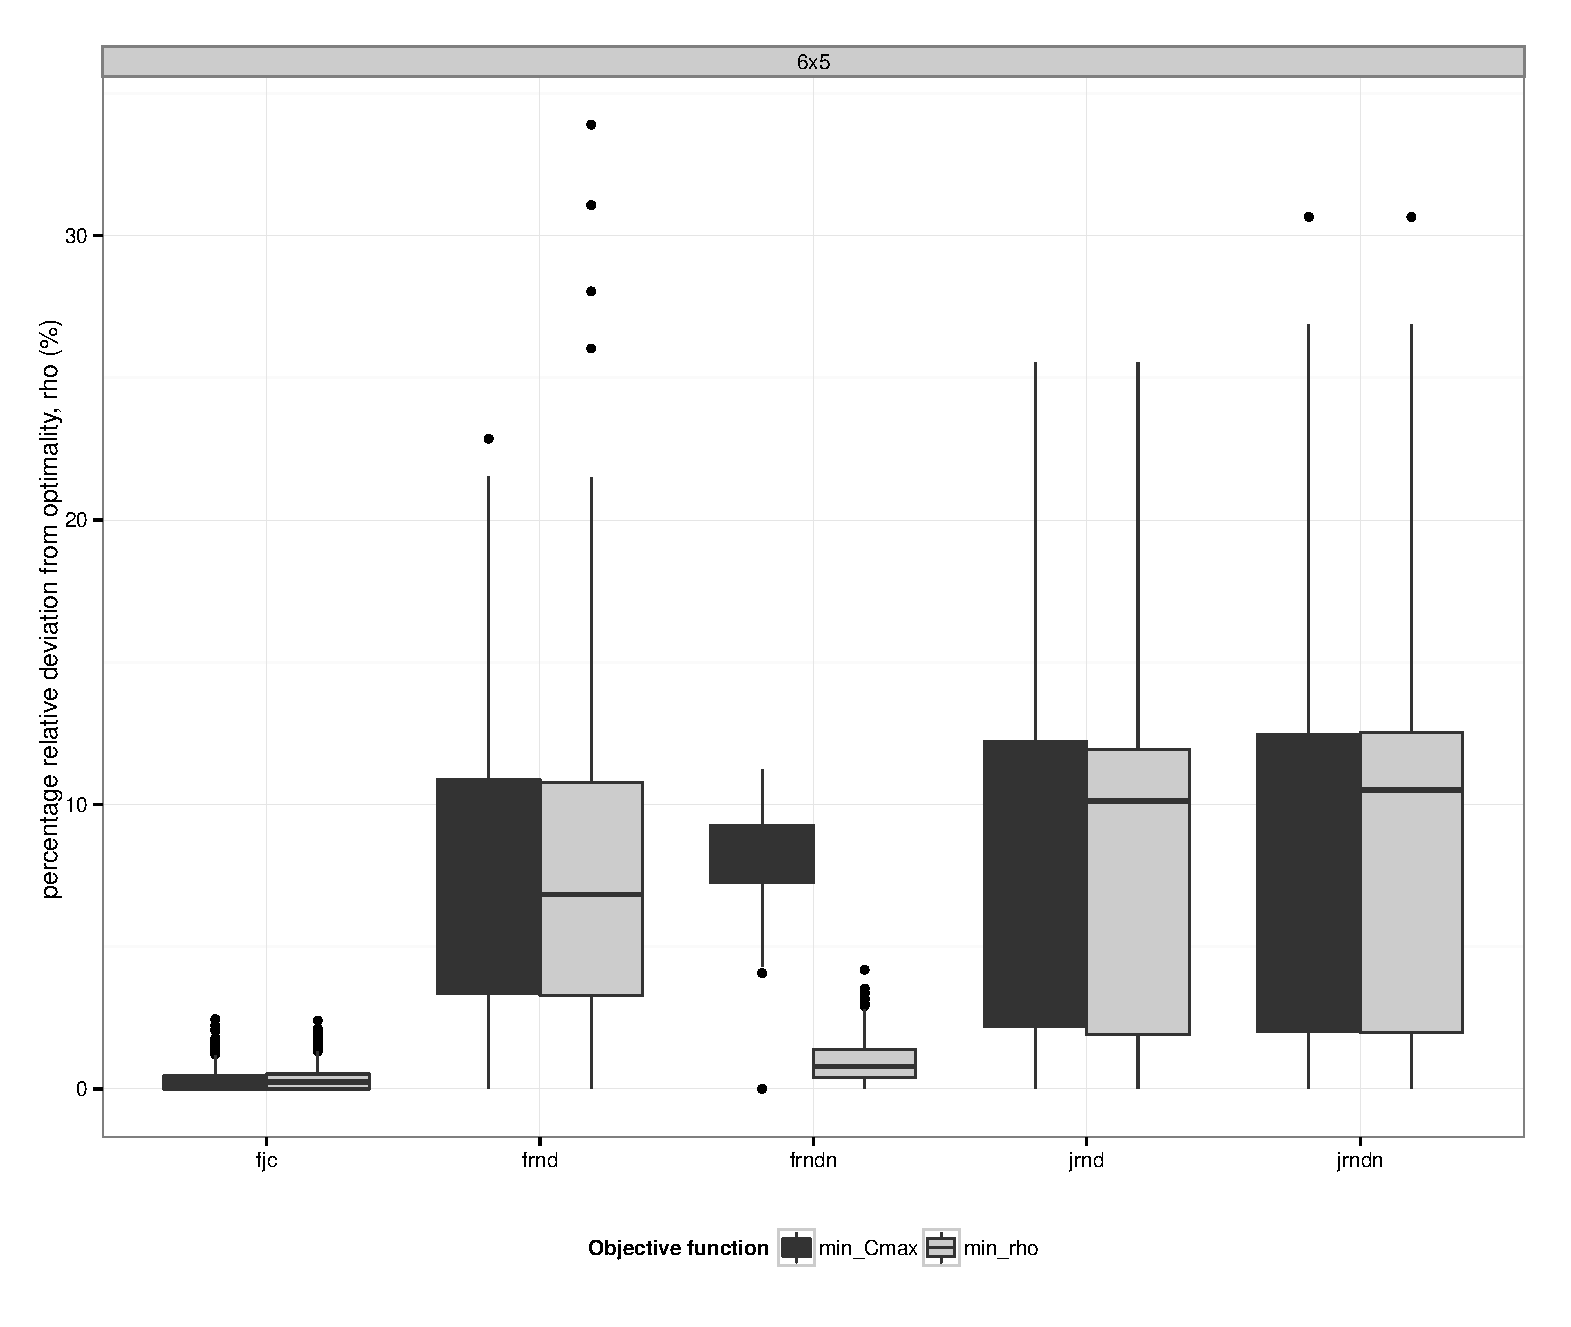
\includegraphics[width=\columnwidth]{CMAboxplotEvoTrain}
	\caption{Box-plot of training data for percentage relative deviation from optimality, defined by \cref{eq:rho}, when implementing the final weights obtained from CMA-ES optimisation, using both objective functions from \cref{eq:cma:makespan,eq:cma:rho}, left and right, respectively.}\label{fig:cma:trainboxpl}
\end{figure}

\subsection{Problem difficulty}\label{sec:expr:data}
The evolution of fitness per generation from the CMA-ES optimisation of \cref{eq:cma:rho} is depicted in \cref{fig:cma:fit}, and since all problem spaces reached their allotted computational time, without converging. In fact \frnd{6}{5} and \jrndn{6}{5} needed restarting during the optimisation process. 
Furthermore, the  evolution of the decision variables, $\vec{w}$, are depicted in \cref{fig:cma:wei}. As one can see, the relative contribution for each weight clearly differs between problem spaces. Note that in the case of \jrndn{6}{5} (cf. \cref{fig:cma:wei:rho}), CMA-ES restarts around generation 1,000 and quickly converges back to its previous fitness, however lateral relation of weights has completely changed. Implying that there are many optimal combinations of weights to be used, which can be expected due  to the fact some features in \cref{tbl:features} are a linear combination of one others, e.g., $\phi_3=\phi_1+\phi_2$.

\begin{figure} 
	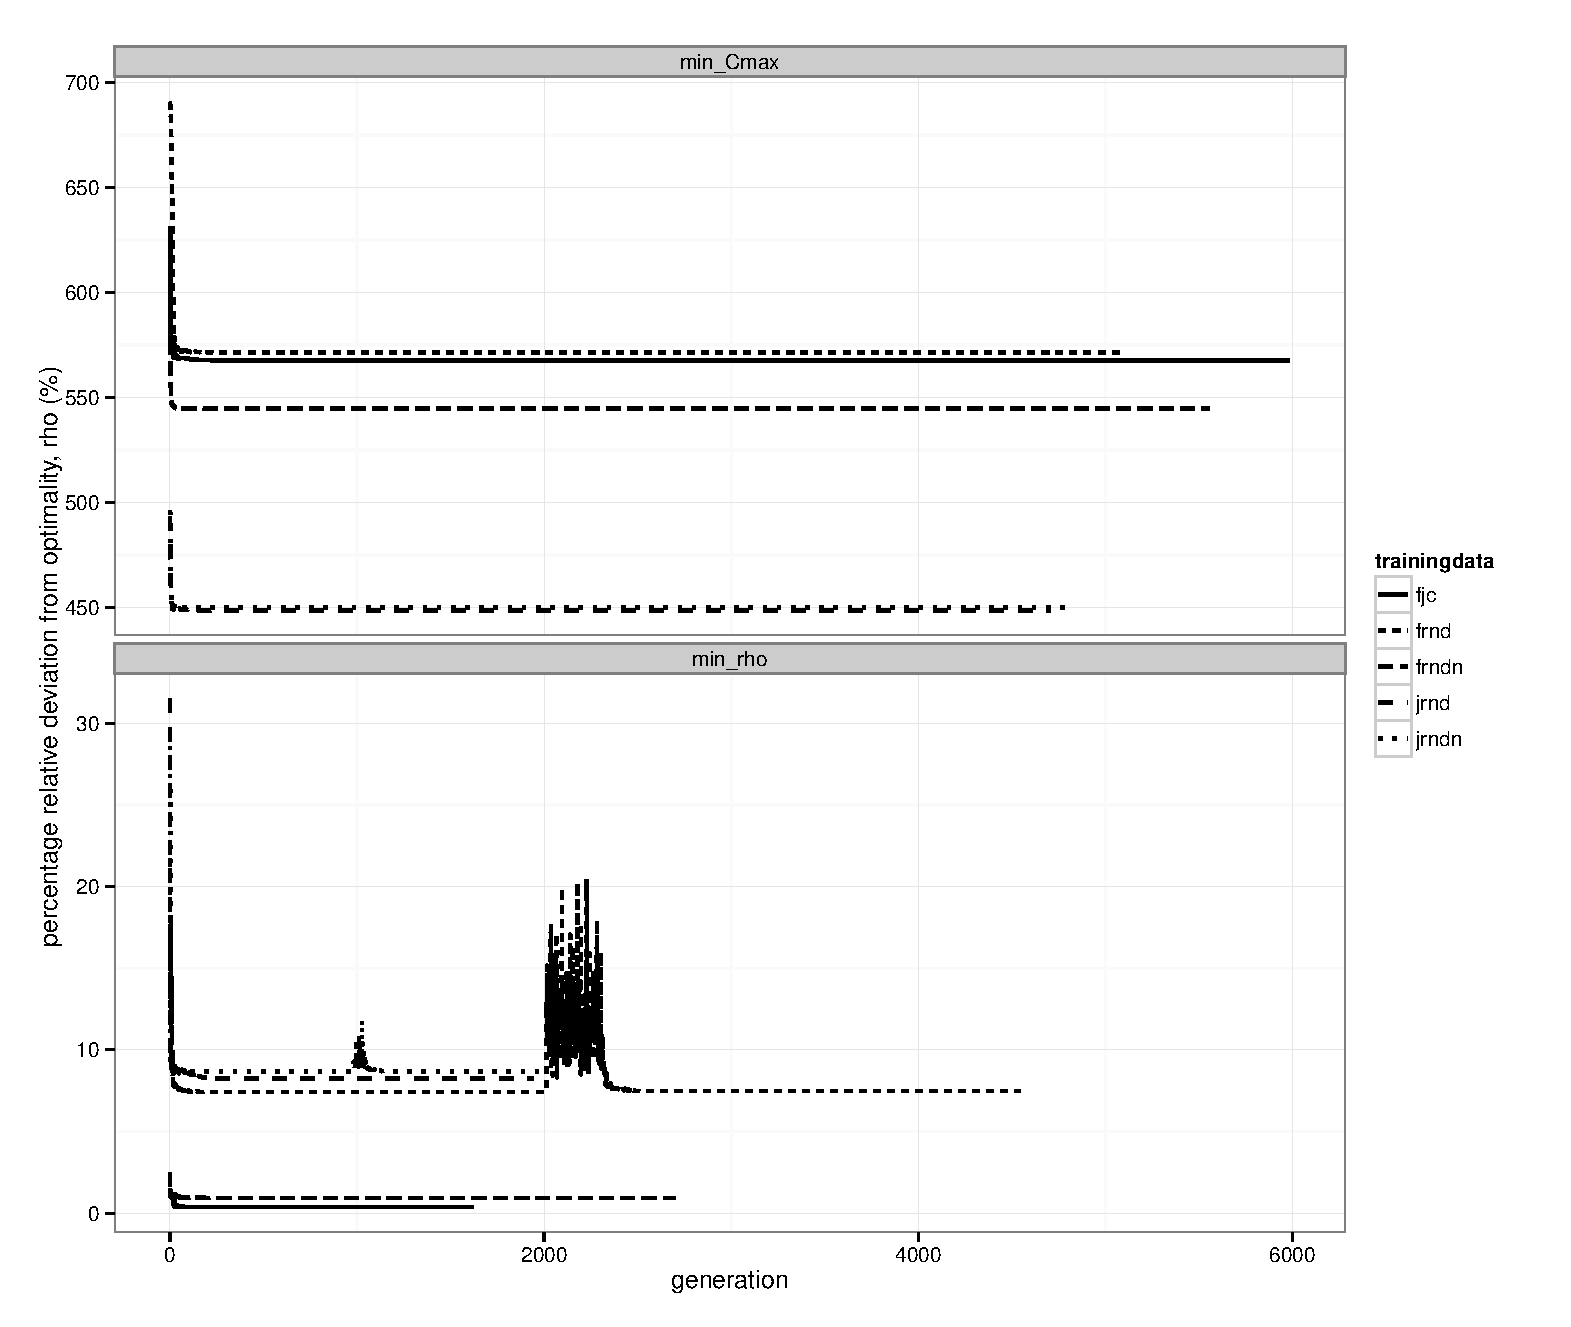
\includegraphics[width=\columnwidth]{CMAfitnessEvo}
	\caption{Fitness for optimising (w.r.t. \cref{eq:cma:makespan,eq:cma:rho} above and below, receptively), per generation of the CMA-ES optimisation.}\label{fig:cma:fit}
\end{figure}

\begin{figure*} 
	\subcaptionbox{minimise w.r.t. \cref{eq:cma:makespan}}{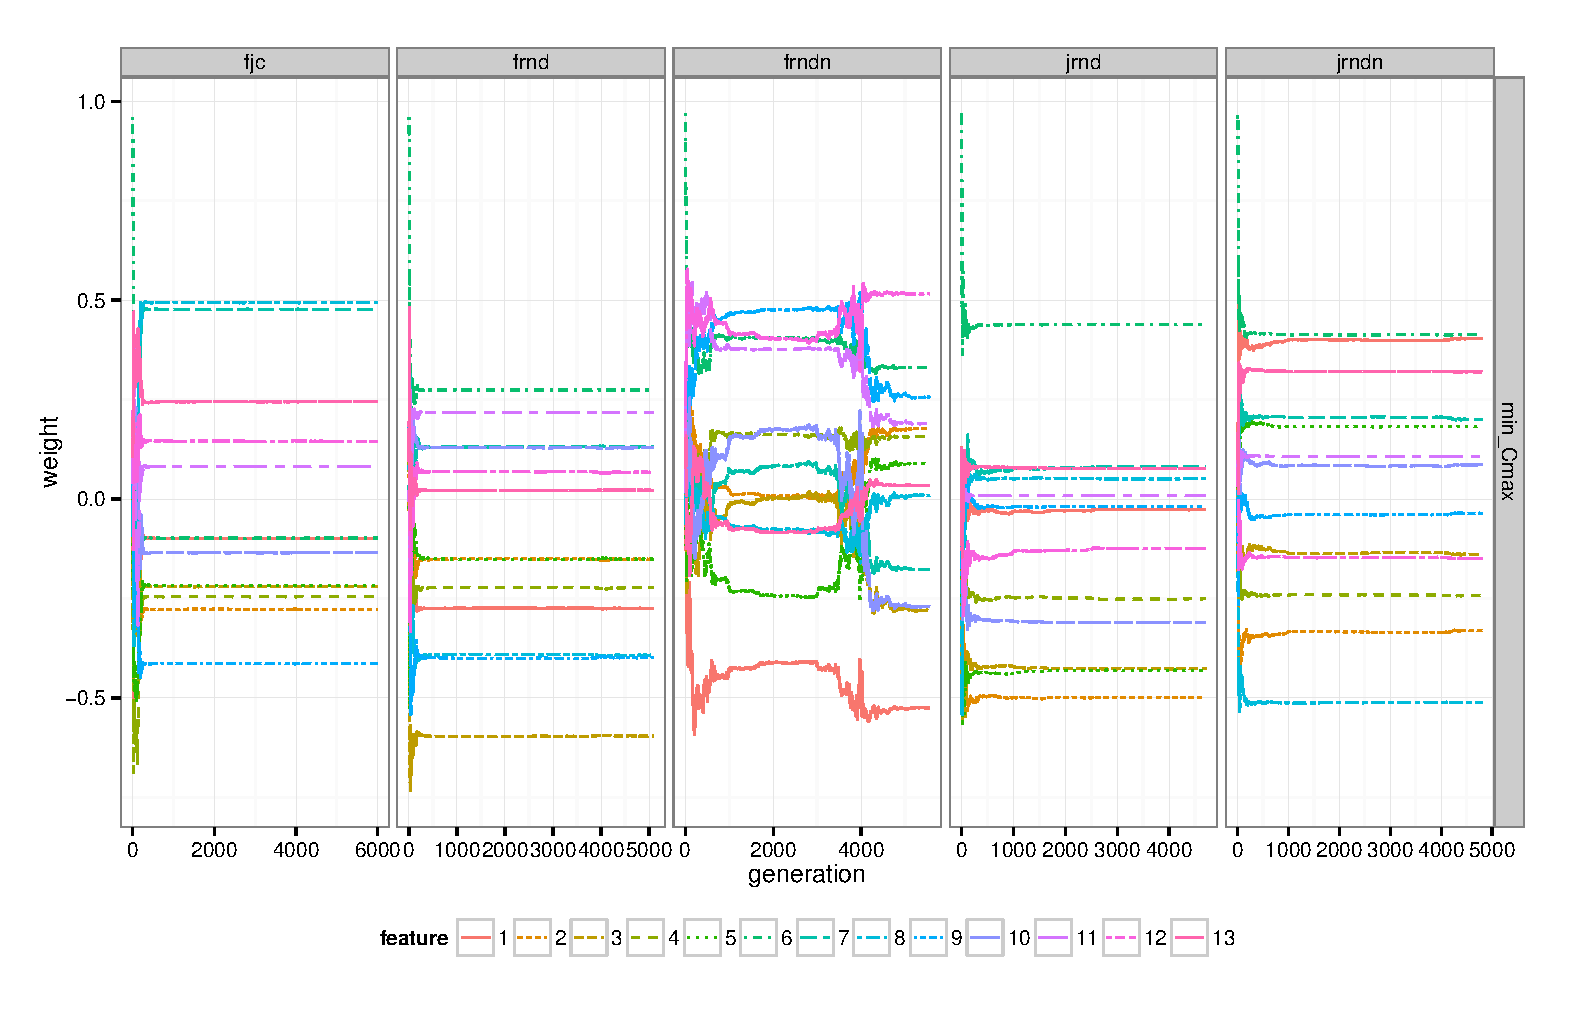
\includegraphics[width=\columnwidth]{CMAweightsEvomin_Cmax}\label{fig:cma:wei:cmax}}
	\\
	\subcaptionbox{minimise w.r.t. \cref{eq:cma:rho}}{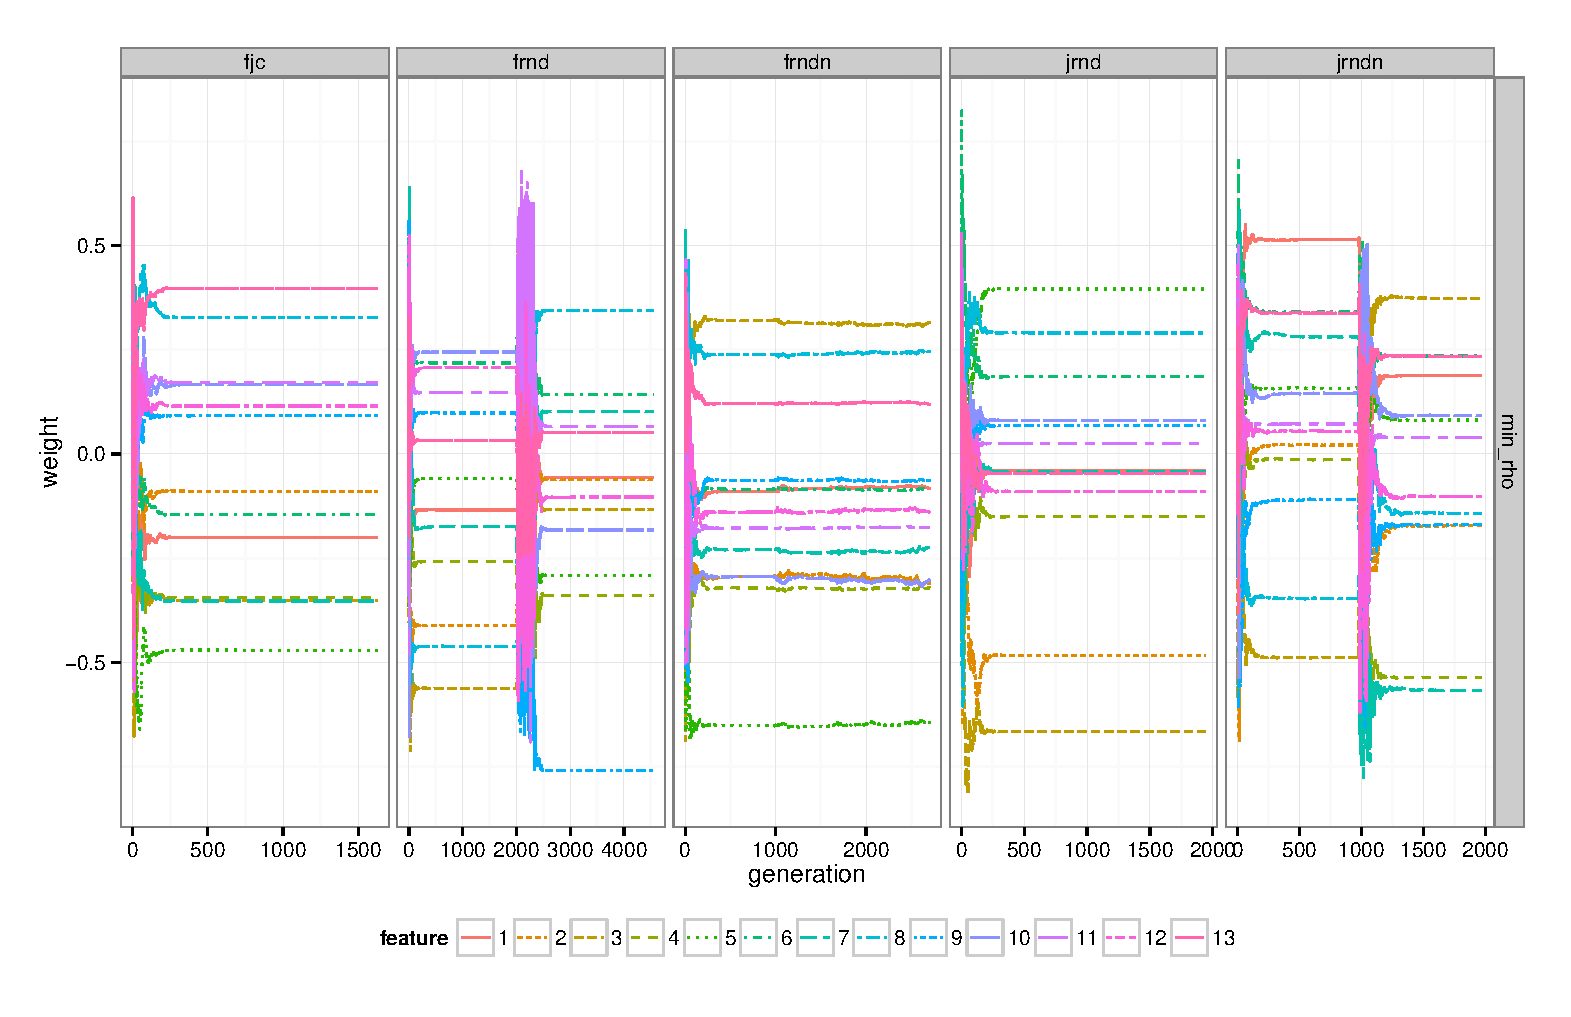
\includegraphics[width=\columnwidth]{CMAweightsEvomin_rho}\label{fig:cma:wei:rho}}
	\caption{Evolution of weights of features (given in \cref{tbl:features}) at each generation of the CMA-ES optimisation. Note, weights are normalised such that $\norm{\vec{w}}=1$.}\label{fig:cma:wei}
\end{figure*}


\subsection{Robustness and  scalability}\label{sec:expr:robust} 
As a benchmark, the linear ordinal regression model (PREF) from \cref{InRu11a} 
was created.
Using the weights obtained from optimising \cref{eq:cma:rho} and applying them on their  $6\times5$ training data, their main statistics of \cref{eq:rho} are reported in \cref{tbl:results:train}, for all training sets described in \cref{tbl:data}. Moreover, the best SDR, from which the features in \cref{tbl:features} were inspired by, are also reported for comparison, i.e., most work remaining (MWR) for all \JSP\ problem spaces, and least work remaining (LWR) for all \FSP\ problem spaces.

To explore the scalability of the learning methods, a similar comparison to \cref{sec:expr:robust} is made for the applying the learning models on their corresponding $10\times10$ testing data, results are reported in \cref{tbl:results:test}. Note that only resulting $C_{\max}$ is reported, as the optimum makespan is not known. 

{\setlength{\tabcolsep}{3pt}
	\begin{table}[p]\centering
\caption{Main statistics of percentage relative deviation from optimality, $\rho$, defined by \cref{eq:rho} for various models, using corresponding $6\times5$ training data.}
\label{tbl:results:train}
%jsp
\subcaptionbox{\jrnd{6}{5}}{\label{tbl:train:j.rnd}
\begin{tabular}{lrrrrr} \toprule
model&mean & med & sd & min & max \\   \midrule
ES$_{C_{\max}}$& 8.54 & 10 &  6 &  0 & 26   \\ % CMA-ES min_Cmax j.rnd 6x5 train
ES$_\rho$& 8.26 & 10 &  6 &  0 & 26   \\ % CMA-ES min_rho j.rnd 6x5 train
PREF&   10.18 & 11 &  7 &  0 & 30  \\ %PREF j.rnd 6x5 train
MWR &  16.48 & 16 &  9 &  0 & 45   \\ %MWR j.rnd 6x5 train
\bottomrule \end{tabular}}
\quad
\subcaptionbox{\jrndn{6}{5}}{\label{tbl:train:j.rndn}
\begin{tabular}{lrrrrr} \toprule
model&mean & med & sd & min & max \\   \midrule
ES$_{C_{\max}}$& 8.68 & 11 &  6 &  0 & 31   \\ % CMA-ES min_Cmax j.rndn 6x5 train
ES$_\rho$& 8.69 & 11 &  6 &  0 & 31   \\ % CMA-ES min_rho j.rndn 6x5 train
PREF&  10.00 & 11 &  6 &  0 & 31   \\ %PREF j.rndn 6x5 train
MWR &  14.02 & 13 &  8 &  0 & 37   \\ %MWR j.rndn 6x5 train
\bottomrule \end{tabular}}
\\
%flow shop
\subcaptionbox{\frnd{6}{5}}{\label{tbl:train:f.rnd}
\begin{tabular}{lrrrrr} \toprule
model&mean & med & sd & min & max \\   \midrule
ES$_{C_{\max}}$& 7.44 &  7 &  5 &  0 & 23   \\ % CMA-ES min_Cmax f.rnd 6x5 train
ES$_\rho$& 7.48 &  7 &  5 &  0 & 34   \\ % CMA-ES min_rho f.rnd 6x5 train
PREF&   9.87 &  9 &  7 &  0 & 38  \\ %PREF f.rnd 6x5 train
LWR &  20.05 & 19 & 10 &  0 & 71   \\ %LWR f.rnd 6x5 train
\bottomrule \end{tabular}}
\quad
\subcaptionbox{\frndn{6}{5}}{\label{tbl:train:f.rndn}
\begin{tabular}{lrrrrr} \toprule
model&mean & med & sd & min & max \\   \midrule
ES$_{C_{\max}}$& 8.09 &  8 &  2 &  0 & 11   \\ % CMA-ES min_Cmax f.rndn 6x5 train
ES$_\rho$& 0.94 &  1 &  1 &  0 &  4   \\ % CMA-ES min_rho f.rndn 6x5 train
PREF&   2.38 &  2 &  1 &  0 &  7  \\ %PREF f.rndn 6x5 train
LWR &  2.25 &  2 &  1 &  0 &  7   \\ %LWR f.rndn 6x5 train
\bottomrule \end{tabular}}
\\
\subcaptionbox{\fjc{6}{5}}{\label{tbl:train:f.jc}
\begin{tabular}{lrrrrr} \toprule
model&mean & med & sd & min & max \\   \midrule
ES$_{C_{\max}}$& 0.33 &  0 &  0 &  0 &  2   \\ % CMA-ES min_Cmax f.jc 6x5 train
ES$_\rho$& 0.36 &  0 &  0 &  0 &  2   \\ % CMA-ES min_rho f.jc 6x5 train
PREF&   1.08 &  1 &  1 &  0 &  5  \\ %PREF f.jc 6x5 train
LWR &  1.13 &  1 &  1 &  0 &  6   \\ %LWR f.jc 6x5 train
\bottomrule \end{tabular}}
\end{table}

	\begin{table}[p]\centering
\caption{Main statistics of $C_{\max}$ for various models, using corresponding $10\times 10$ test data.}
\label{tbl:results:test}
%jsp
\subcaptionbox{\jrnd{10}{10}}{\label{tbl:test:j.rnd}
\begin{tabular}{lrrrrr}  \toprule
model&mean & med & sd & min & max \\ 
  \midrule
ES$_{C_{\max}}$& 922.51 & 914 & 73 & 741 & 1173   \\ % CMA-ES min_Cmax j.rnd 10x10 test
ES$_\rho$& 931.37 & 931 & 71 & 735 & 1167   \\ % CMA-ES min_rho j.rnd 10x10 test
  PREF&   1011.38 & 1004 & 82 & 809 & 1281 \\   %PREF j.rnd 10x10 test
  MWR &  997.01 & 992 & 81 & 800 & 1273   \\ %MWR j.rnd 10x10 test
\bottomrule \end{tabular}}
\quad
\subcaptionbox{\jrndn{10}{10}}{\label{tbl:test:j.rndn}
\begin{tabular}{lrrrrr} \toprule
model& mean & med & sd & min & max \\ 
  \midrule
ES$_{C_{\max}}$& 855.85 & 857 & 50 & 719 & 1010   \\ % CMA-ES min_Cmax j.rndn 10x10 test
ES$_\rho$& 855.91 & 856 & 51 & 719 & 1020   \\ % CMA-ES min_rho j.rndn 10x10 test
  PREF&   899.94 & 898 & 56 & 769 & 1130  \\ %PREF j.rndn 10x10 test
  MWR&  897.39 & 898 & 56 & 765 & 1088   \\ %MWR j.rndn 10x10 test
\bottomrule \end{tabular}}
\\
%flow shop
\subcaptionbox{\frnd{10}{10}}{\label{tbl:test:f.rnd}
\begin{tabular}{lrrrrr} \toprule
model&mean & med & sd & min & max \\   \midrule
ES$_{C_{\max}}$& 1178.73 & 1176 & 80 & 976 & 1416   \\ % CMA-ES min_Cmax f.rnd 10x10 test
ES$_\rho$& 1181.91 & 1179 & 80 & 984 & 1404   \\ % CMA-ES min_rho f.rnd 10x10 test
PREF&  1215.20 & 1212 & 80 & 1006 & 1450  \\ %PREF f.rnd 10x10 test
LWR &  1284.41 & 1286 & 85 & 1042 & 1495   \\ %LWR f.rnd 10x10 test
\bottomrule \end{tabular}}
\quad 
\subcaptionbox{\frndn{10}{10}}{\label{tbl:test:f.rndn}
\begin{tabular}{lrrrrr} \toprule
model&mean & med & sd & min & max \\   \midrule
ES$_{C_{\max}}$& 1065.48 & 1059 & 32 & 992 & 1222   \\ % CMA-ES min_Cmax f.rndn 10x10 test
ES$_\rho$& 980.11 & 980 &  8 & 957 & 1006   \\ % CMA-ES min_rho f.rndn 10x10 test
PREF&  987.49 & 988 &  9 & 958 & 1011  \\ %PREF f.rndn 10x10 test
LWR &  986.94 & 987 &  9 & 959 & 1010   \\ %LWR f.rndn 10x10 test
\bottomrule \end{tabular}}
\\
\subcaptionbox{\fjc{10}{10}}{\label{tbl:test:f.jc}
\begin{tabular}{lrrrrr} \toprule
model&mean & med & sd & min & max \\   \midrule
ES$_{C_{\max}}$& 1135.44 & 1134 & 286 & 582 & 1681   \\ % CMA-ES min_Cmax f.jc 10x10 test
ES$_\rho$& 1135.47 & 1134 & 286 & 582 & 1681   \\ % CMA-ES min_rho f.jc 10x10 test
PREF&   1136.02 & 1135 & 286 & 582 & 1685 \\  %PREF f.jc 10x10 test
LWR &  1136.49 & 1141 & 287 & 581 & 1690   \\ %LWR f.jc 10x10 test
\bottomrule \end{tabular}}
\end{table}}

\section{Discussion and conclusions}\label{sec:disc}
Data distributions considered in this study either varied 
w.r.t. the processing times distributions, continuing the preliminary 
experiments in  \cref{InRu11a} , or 
w.r.t. the job ordering permutations, i.e., homogeneous $\sigma$ matrices in \FSP\ versus heterogeneous $\sigma$ matrices in \JSP . 
From the results based on $6\times5$ training data, given  in 
\cref{tbl:results:train}, it's obvious that CMA-ES optimisation substantially 
outperforms the previous PREF methods from \cref{InRu11a}, for all problem 
spaces considered. Furthermore, the results hold when testing on $10\times10$, 
(cf. \cref{tbl:results:test}), suggesting the method is indeed  scalable for 
higher dimensions. 

Moreover, the study showed that the choice of objective function  for 
evolutionary search is worth investigating. There was no statistical difference 
from minimising the fitness function directly and its normalisation w.r.t. true 
optimum (cf. \cref{eq:cma:makespan,eq:cma:rho}), save for \frndn{6}{5}. 
Implying, even though ES doesn't rely on optimal solutions, there are some 
problem spaces where it can be of great benefit. This is due to the fact that 
the problem instances can vary greatly within the same problem space 
\cref{InRu12}, thus normalising the objective function would help the 
evolutionary search to deviate the from giving too much weight for problematic 
problem instances for the greater good.

The weights for \cref{eq:CDR:feat} in \cref{InRu11a} were found using 
supervised learning, where the training data was created from optimal solutions 
of randomly generated problem instances. As an alternative, this study showed  
that minimising the mean makespan directly using a brute force search via 
CMA-ES actually results in a better CDRs. The nature of CMA-ES is to explore 
suboptimal routes until it converges to an optimal one. Implying that the 
previous approach of only looking into one optimal route may not produce a 
sufficiently rich training set. That is, the training set should incorporate a 
more complete knowledge on \emph{all} possible preferences, i.e., make also the 
distinction between suboptimal and sub-suboptimal features, etc.  This would 
require a Pareto ranking of preferences which can be used to make the 
distinction to which feature sets are equivalent, better or worse -- and to 
what degree, i.e., by giving a weight to the preference. This would result in a 
very large training set, which of course could be re-sampled in order to make 
it computationally feasible to learn.

The main drawback of using evolutionary search for learning optimal weights for 
\cref{eq:CDR:feat} is how computationally expensive it is to evaluate the mean 
expected fitness. Even for a low problem dimension, 6-job 5-machine \JSP , each 
optimisation run reached their walltime of 288hrs, without converging. Now, 
$6\times5$ \JSP\ requires 30 sequential dispatches, where at each time step 
there are up to $6$ jobs to choose from, i.e., its complexity is 
$\mathcal{O}(n^{n\cdot m})$, making it computationally infeasible to apply this 
framework for higher dimensions as is. 
However, evolutionary search only requires the rank of the candidates, and 
therefore it is appropriate to retain a sufficiently accurate surrogate for the 
value function during evolution in order to reduce the number of costly true 
value function evaluations, such as the approach in \cref{InRu11b}. This could 
reduce the computational cost of the evolutionary search considerably, making 
it feasible to conduct the experiments from \cref{sec:es:measure} for problems 
of higher dimensions, e.g., with these adjustments it is possible to train on 
$10\times10$ and test on for example $14\times14$ to verify whether scalability 
holds for even higher dimensions.  





 %ch.8
\HeaderQuote{The adventures first... explanations take such a dreadful time.}{The Gryphon} %Alice's Adventures in Wonderland:


\chapter{Experiments }\label{ch:experiments} 
\todoWrite{Compare CMA-ES to PREF models}

\FirstSentence{T}{here's something to be said} for having a good opening line. Morbi commodo, ipsum sed pharetra gravida, orci  $x = 1/\alpha$ magna rhoncus neque, id pulvinar odio lorem non turpis. Nullam sit amet enim. Suspendisse id velit vitae ligula volutpat condimentum. Aliquam erat volutpat. Sed quis velit. Nulla facilisi. Nulla libero. Vivamus pharetra posuere sapien. Nam consectetuer. Sed aliquam, nunc eget euismod ullamcorper, lectus nunc ullamcorper orci, fermentum bibendum enim nibh eget ipsum. Donec porttitor ligula eu dolor. Maecenas vitae nulla consequat libero cursus venenatis. Nam magna enim, accumsan eu, blandit sed, blandit a, eros.
$$\zeta = \frac{1039}{\pi}$$

\clearpage

\Cref{jsp:methods} summarise the main techniques applied to solve \JSP. The 
figure is based on Fig. 1 from \citet{Jain99}, however, updated to reflect the 
previous work relevant to this dissertation.

Some notes
\begin{description}
    \item[Local Search] \cite{LocalSearch} divide approximations methods to 
    \begin{enumerate}
        \item iterative methods, which starts with some initial feasible 
        solution, and its neighbourhood is searched for one with lower cost. If 
        such a solution is found, the algorithm is
        continued from there; otherwise, a local minimum has been found
        \item constructive methods, construct a complete schedule and apply 
        local search to partial schedules on the way
    \end{enumerate}
    \item[Greedy randomized adaptive search procedure] (GRASP) for \JSP\ by 
    \cite{GRASP}
    \item[Beam search] by \cite{BeamSearch} is an adaptation of the branch and 
    bound method in which only some nodes are evaluated in the search tree. At 
    any level, only the promising nodes are kept for further branching and 
    remaining nodes are pruned off permanently.
    \item[Insertion Algorithm] \cite{InsertionAlg} 
\end{description}


\clearpage
%http://tex.stackexchange.com/questions/244742/work-breakdown-structure-wbs-horizontally

\usetikzlibrary{shapes,positioning,shadows,trees}

\tikzset{arrow/.style = {->,>={latex}, draw=black},
        txtLrg/.style  = {draw, text width=2cm, align=center, %drop shadow, 
            font=\bfseries\scriptsize\sffamily, rectangle, thin},
        txtSml/.style  = {txtLrg, align=left, 
            font=\tiny\sffamily},
        txtComment/.style = {font=\tiny\sffamily, xshift=-0.4cm, near start,
            text width=4cm, rotate=90, align=left},
        txtRef/.style= {font=\tiny\sffamily, midway, above, sloped},
        hybrid/.style = {-,draw=black, dashed},
        based/.style = {arrow, dotted},
        veryshort/.style = {text width=3em},
        short/.style = {text width=4.25em},
        medium/.style = {text width=7em},
        long/.style = {text width=7em},
        verylong/.style = {text width=8em},
}

\forestset{
    normal/.style  = {for tree={child anchor=west, parent anchor=east}},
    rotated/.style = {for tree={child anchor=north, parent anchor=south},
        rotate=90},
    unrotate/.style = {normal, rotate=-90},
    root/.style  = {txtLrg, rotated, fill=gray!50, medium},
    onode/.style = {txtLrg, rotated, fill=gray!25, medium},
    tnode/.style = {txtSml, normal, fill=gray!10, long},
    emphasis/.style = {}, %tikz={\node [draw,red,thick,fit to tree]{};}},
    edge from parent/.style={arrow, edge from parent fork right}
}

\begin{figure}[p] \centering
\begin{forest}
for tree={
    s sep=3pt, % distance between siblings
    grow=east,
    growth parent anchor=east,
    edge path={\noexpand\path[\forestoption{edge},->, >={latex}] 
        (!u.parent anchor) -- +(5pt,0pt) |- (.child anchor)
        \forestoption{edge label};}
}
[\JSP, root
    [Approximation, root, edge label = {node[txtComment, left]{
            Approximations methods, or heuristics, are generally time 
            efficient, but do not necessarily attain the global optimum.}},
        [General algorithms (iterative methods), onode, verylong
            [Artificial intelligence, onode
                [Machine learning, onode,  
                    [Roll-out / Pilot method, tnode]
                    [Reinforcement learning, tnode]
                    [Decision tree, tnode]
                    [Imitation learning, onode, emphasis
                        [Active, onode, veryshort
                            [DAgger, tnode, short]
                        ]
                        [Passive, onode, veryshort
                            [Follow the expert, tnode, short]
                            [Perturbed leader, tnode, short]
                            [Follow heuristics, tnode, short]
                        ]
                    ]
                ]
                [Constraint satisfaction,tnode]
%                [Expert systems,tnode]
                [Ant colony optimisation,tnode, name=ACO]
                [Artificial neural network,tnode, name=ANN]
            ]
            [Local search, onode
                [Reinsertion algorithms, tnode]
                [Threshold alg., onode, long, unrotate
                    [Simulated annealing, tnode, name=SA]
                    [Threshold accepting, tnode
%                        [Great Deluge alg. \& record-to-record travel, tnode]
                    ]
                    [Iterative development, tnode]
                ]
%                [Problem space methods, onode
%                    [Problem and heuristic space, tnode]
%                    [GRASP, tnode]
%                ]
                [Large step optimisation, tnode]
                [Tabu Search, tnode, name=TS]
                [Evolutionary computation,tnode
                    [Genetic local search, tnode]
                ]
                [Genetic algorithms, tnode, name=GA
                    [Genetic programming, tnode, name=GP]
                ]
                [Variable depth search, tnode, name=VDS]
            ]
        ]
        [Tailored algorithms (constructive methods), onode, verylong
            [Bottleneck based heuristics, onode, long, unrotate
                [Shifting bottleneck procedure, tnode, short, name=SBP
                    [Beam search, tnode, short, name=BS]
                ]
            ]
            [Insertion algorithm, tnode, veryshort]
            [Priority DR, onode, short, emphasis
                [SDR, onode, short
                    [SPT, tnode, veryshort]
                    [LPT, tnode, veryshort]
                    [LWR, tnode, veryshort]
                    [MWR, tnode, veryshort]
                ]
                [CDR, tnode, name=CDR, veryshort]
            ] 
         ]
    ]
    [Optimisation, root, edge label = {node[txtComment, right]{
            Exact methods guarantee an optimal solution, although for NP-hard 
            problems they are intractable for high dimensionality.}},
        [Efficient methods, tnode, short] 
        [Enumerative methods, onode, 
            [Branch \& Bound, tnode, name=BB]
            [Mathematical, onode
                [Surrogate duality, tnode] 
                [Lagrangian relaxation, tnode] 
                [Decomposition methods, tnode] 
                [Integer linear programming, tnode] 
                [Mixed integer lin.prog., tnode] 
            ]
        ]
    ]
]
\draw[arrow] (ANN) -| (SA);
\draw[arrow] (VDS) -| (SBP);
%\draw[based,out=east,in=north] (BB) to node[txtRef] {\cite{BeamSearch}} (BS);
%\draw[hybrid,out=east,in=east] (GA) to (TS);
%\draw[based,out=east,in=east]  (ACO) to node[txtRef] {\cite{Korytkowski13}} 
%(CDR) ;
%\draw[based,out=east,in=east] (GP) to (CDR);
\end{forest}
\caption[Various methods for solving \JSP]{Various methods for solving \JSP\ 
\citep[based on Fig. 1 from][]{Jain99}}\label{jsp:methods}
\end{figure}
\begin{table}[p] \centering
    \caption{Summary of experimental designs in \namecref{InRu11a}s.}
    \label{papers:summary}
    \subcaptionbox{Model parameters\label{papers:models}}{
    \begin{minipage}{\fullwidth}\centering
    {\setlength{\tabcolsep}{3pt}
    \begin{tabular}{c l c l c}\toprule
        Paper & Problem & Model & Model parameters 
        & $\abs{\text{Model}}$\footnote{Models are either stepwise (i.e. 
            total of $K$ models) or fixed throughout the dispatching 
            process.} \\ \midrule
        \ref{InRu11a} & \JSP & PREF & 
        ~~$\Phi^{\text{OPT}}, \Psi_b$ & $K$ \\
        \ref{InRu11b} & $\R$-functions & CMA-ES & 
        ~~surrogate sampling strategies & 1\\
        \ref{InRu12} & \JSP& SDR & 
        ~~MWR & 1 \\
        \ref{InRu14} & \JSP, \FSP & CMA-ES & 
        ~~$\min \Exp{C_{\max}},\min \Exp{\rho}$ & 1 \\
        \ref{InRu15a} & \JSP & PREF & 
        $\!\begin{array}{l}
            \condset{\Phi^\pi}{\pi\in\{\text{OPT},\text{SDR},\text{ALL}\}}\\
            \condset{\Psi_r}{r\in\{b,f,p\}}
        \end{array}$
        & $K$\\
        \ref{InRu15b} & \JSP, \FSP & PREF & 
        ~~$\Phi^{\text{OPT}},\Psi_p$ & 1\\
        \ref{InRu15c} & \JSP, \FSP & PREF & 
        $\!\begin{array}{l}
            \condset{\Phi^\pi}{\pi\in\{\text{OPT},\text{OPT}\epsilon,\text{DA}i\}}\\
            \Psi_p
        \end{array}$
        & 1 \\
        \bottomrule
    \end{tabular}}
    \end{minipage}}
    \\
    \subcaptionbox{\JSP\ and  \FSP\ problems spaces\label{papers:problems}}{
    \begin{minipage}{\fullwidth}\centering
    {\setlength{\tabcolsep}{3pt}
    \begin{tabular}{c l l l l}\toprule
      Paper & Problem & $I=[u_1,u_2]$\footnote{Processing times are uniformly
        distributed from an interval $I=[u_1,u_2]$, i.e., 
        $\vec{p}\sim\mathcal{U}(u_1,u_2)$.} & size ($n\times m$) & name \\ 
        \midrule
      \ref{InRu11a} & \JSP & $[1,100], [50,100]$ & $6\times6$ & j.rnd, j.rndn\\
      \ref{InRu12} & \JSP & $[1,200]$ & $6\times 6$ & j.rnd \\
      \ref{InRu14} & \JSP, \FSP & $[1,99],[45,55]$ & $6\times5,10\times10$ & 
      j.rnd, j.rndn, f.rnd, f.rndn, f.jc\\
      \ref{InRu15a} & \JSP & $[1,99],[45,55]$ & $6\times5$ & j.rnd, j.rndn\\
      \ref{InRu15b} & \JSP, \FSP & $[1,99],[45,55]$ & $10\times10$ & 
      j.rnd, j.rndn, f.rnd\\
      \ref{InRu15c} & \JSP, \FSP & $[1,99],[45,55]$ & $6\times5,10\times10$ & 
      j.rnd, j.rndn, f.rnd\\
      \bottomrule
    \end{tabular}}
    \end{minipage}}
\end{table}
 %ch.9
\HeaderQuote{Tut, tut, child! Everything's got a moral, if only you can find it.}{The Duchess} 

\chapter{Conclusions}\label{ch:conclusions} 
\FirstSentence{C}{urrent literature still hold} \sdr s in high regard, as they 
are simple to implement and quite efficient. 
However, they are generally taken for granted as there is clear lack of 
investigation of \emph{how} these \dr s actually work, and what 
makes them so successful (or in some cases unsuccessful)? 

For instance, of the four SDRs from \cref{sec:SDR} this dissertation focused 
on, why does MWR outperform so significantly for \jsp\, yet completely fail for 
\fsp? 
MWR seems to be able to adapt to varying distributions of processing times, 
however, manipulating the machine ordering causes MWR to break down. 
By inspecting optimal schedules, and meticulously researching what's going on, 
every step of the way of the dispatching sequence as was done in 
\cref{ch:analysingsol}, some light is shed where these SDRs vary w.r.t. the 
problem space at hand. 
Once these simple rules are understood, then it's feasible to extrapolate the 
knowledge gained and create new \cdr s that are likely to be successful. 
An example of which was a blended \dr\ in \cref{sec:diff:opt:bdr}, where we 
start with the SPT heuristic and switch over to MWR at a predetermined time 
points. Those pivotal time steps were chosen by inspecting where SPT succeeds 
MWR (and vice versa). 
By achieving a higher classification accuracy using the new BDR model, it 
substantially improve its inherited rule SPT.
Although, it doesn't transcend to a significantly lower \namerho, when compared 
to its other inherited rule MWR. 
Special care must be taken not to let SPT downgrade MWR performance. This can 
be avoided by inspecting how $\rho$ is evolving as a function of time (cf. 
\cref{fig:diff:case:SDR}) and only consider swapping trajectories before they 
intersect and subsequently diverge in performance. 
Moreover, the improved classification accuracy is proportional to its 
difference in performance spread (i.e. 
$\abs{\zeta^{\MWR}_{\any} - \zeta^{\SPT}}_{\any}$) in that region.

Creating new \dr s is by no means trivial. For \jsp\ there is 
the hidden interaction between processing times and machine ordering that's 
hard to measure.
Due to this artefact, feature selection is of paramount importance, and then it 
becomes the case of not having too many features, as they are likely to hinder 
generalisation due to over-fitting in training the preference model, as was 
seen in \cref{sec:trdat:param:tracks:passive}. 
However, the features need to be explanatory enough to maintain predictive 
ability. 
For this reason \cref{eq:CDR:feat} was limited to up to three active features 
in \cref{sec:pref:featselect}, as the full feature set was clearly suboptimal 
w.r.t. its CMA-ES benchmark from \cref{ch:esmodels}. 
By using features based on the SDRs, along with some additional local features 
describing the current schedule, it was possible to `discover' the SDRs when 
given only one active feature. 
Although there is not much to be gained by these models, they at least serve as 
a sanity check for the learning models are on the right track. 
Furthermore, by adding on additional features, a boost in performance was 
gained, resulting in a \cdr\ that outperformed all of the SDR baseline. 
Although, the best preference model of 3 active features is still not better 
than the CMA-ES model for \jrnd{10}{10} using \NrFeatLocal\ features. 
However, we're starting to close in on the gap, as previously 
$\Delta\rho\approx6\%$ (using $\Psi_p^{\minCmax}$ from 
\cref{sec:trdat:param:tracks:passive}) and now $\Delta\rho\approx2\%$ (using 
CDR \#3.524 from \cref{tbl:CDR:pareto}) in favour of evolutionary search (cf. 
\cref{tbl:cma:boxplot:set}).



We saw in \cref{sec:trdat:param:tracks:passive} that preference models using 
training data from following SDR policy, i.e., $\Phi^{\SDR}$, are good for 
improving its original heuristic. However, this did not transcend for 
$\Psi^{\CMAES}$. 
Perhaps, if $\Phi^{\CMAES}$ wasn't based on following 
the CMA-ES trajectory, but rather using the actual features encountered during 
its optimisation. Alas, CMA-ES used a computational budget of 50,000 function 
evaluations, each consisting of the expectation of $N_{\train}$ problem 
instances. So even though \cref{fig:cma:fit} becomes relatively stable after a 
few generations, it would still yield a gigantic feature set that needs to be 
filtered before going through the optimisation phase of correctly labelling 
them.

The analysis-phase of \Alice\ is heavily dependent on having an expert 
policy one wants to mimic, i.e., knowing the \emph{optimal} solutions for the 
sake of imitation learning. 

Understandably, knowing the true optimum is an unreasonable claim in many 
situations, especially for high dimensional problem instances. 
Luckily, there seems to be the possibility to circumvent querying the expert 
altogether, and still have reasonable performance. 
By applying \emph{locally optimal learning to search} \citep{ChangKADL15} it is 
possible to use imitation learning even when the reference policy is poor. 
Although it's noted that the quality (w.r.t near-optimality) of reference 
policy is in accordance to its performance, as is to be expected. 

\todoWrite{Write overall conclusions of dissertation!}
 %ch.10

% Back matter
\HeaderQuote{A cat may look at a king. I've read that in some book, but I don't 
remember where.}{Alice}
\begin{references}
    \bibliography{papers/references}
\end{references}

\appendix
\HeaderQuote{What is the use of repeating all that stuff, if you don't explain it as you go on? It's by far the most confusing thing I ever heard!}{The Mock Turtle} 

\chapter{Ordinal Regression}\label{ch:ordinal} 
\FirstSentence{O}{rdinal regression has been} previously presented in 
\cite{Ru06:PPSN}, but given here for completeness. The preference learning task 
of linear classification presented there is based on the work proposed in 
\citep{main:LIBLINEAR,Lin08:newtontrustregion}. 
The modification relates to how the point pairs are selected and the fact that 
a $L2$-regularized logistic regression is used. \todoFind{Cite what is 
L2-regression}

\section{Preference set}
The ranking problem is specified by a \emph{preference set}, 
\begin{equation}
\Psi := \{(\vec{x}_i,y_i)\}_{i=1}^N \subset X \times Y
\end{equation}
consisting of $N$ (solution, rank)-pairs, where $Y=\{r_1,\ldots,r_N\}$ 
is the outcome space with ordered ranks $r_1> r_2,> \ldots > r_N$.  

Now consider the model space $\mathcal{H} = \{h(\cdot) : X \mapsto Y\}$ of 
mappings from solutions to ranks. Each such function $h$ induces an ordering 
$\succ$ on the solutions  by the following rule,
\begin{equation}\label{eq:linear}
	\vec{x}_i \succ \vec{x}_j \quad \Leftrightarrow \quad h(\vec{x}_i) > h(\vec{x}_j)
\end{equation}
where the symbol $\succ$ denotes `is preferred to.' 

In ordinal regression the task is to obtain function $h$ that can for a given pair $(\vec{x}_i,y_i)$ and $(\vec{x}_j,y_j)$ distinguish between two different outcomes: $y_i > y_j$ and $y_j > y_i$. The task is, therefore, transformed into the problem of predicting the relative ordering of all possible pairs of examples \citep{Herbrich00,Joachims02}.  However, it is sufficient to consider only all possible pairs of adjacent ranks (see also \cite{ShaweTaylor04:book} for yet an alternative formulation).  The preference set, composed of pairs, is then as follows,
\begin{equation}
	\Psi = \left\{(\vec{x}_k^{(1)}, \vec{x}_k^{(2)}),t_k=\text{sign}(y_k^{(1)} - 
	y_k^{(2)})\right\}_{k=1}^{N'} \subset X\times Y  \label{eq:PrefSet:problem}
\end{equation}
where $(y_k^{(1)} = r_i) \wedge (y_k^{(2)} = r_{i+1})$, and vice versa 
$(y_k^{(1)} = r_{i+1}) \wedge (y_k^{(2)} = r_{i})$, resulting in $N'=2(N-1)$ 
possible adjacently ranked preference pairs. The rank difference is denoted by 
$t_k\in\{-1,1\}$.

In order to generalize the technique to different solution data types and model 
spaces an implicit kernel-defined feature space $\Phi\subset\mathbb{R}^d$ of 
dimension $d$, with corresponding feature mapping $\vphi:X\mapsto\Phi$ is 
applied, i.e., the feature vector 
$\vphi(\vec{x})=[\phi_1(\vec{x}),\ldots,\phi_d(\vec{x})]^T\in\Phi$. Thus the 
preference set defined by \cref{eq:PrefSet:problem} is redefined as follows,
\begin{equation}
	\Psi = \left\{\left(\vphi(\vec{x}_k^{(1)}), 
	\vphi(\vec{x}_k^{(2)})\right),t_k=\text{sign}(y_k^{(1)} - 
	y_k^{(2)})\right\}_{k=1}^{N'} \subset \Phi \times Y \label{eq:PrefSet:feat}.
\end{equation}


\section{Linear preference}\label{sec:ord:linpref}
The function used to induce the preference is defined by a linear function in the kernel-defined feature space,
\begin{equation} 
  h(\vec{x}) = \sum_{i=1}^d w_i\phi_i(\vec{x})=\inner{\vec{w}}{\vphi(\vec{x})} 
               \label{eq:pref:kernel}
\end{equation}
where $\vec{w}=[w_1,\ldots,w_d]\in\mathbb{R}^d$ has weight $w_i$ for feature $\phi_i$.


\begin{comment}
Let $\vec{z}$ denote either $\vphi(\vec{x}_k^{(1)})-\vphi(\vec{x}_k^{(2)})$ with \mbox{$t_k=+1$} or 
$\vphi(\vec{x}_k^{(2)})-\vphi(\vec{x}_k^{(1)})$ with \mbox{$t_k=-1$}, positive or negative example respectively.

Logistic regression learns the optimal parameters $\vec{w}\in\mathbb{R}^d$ determined by solving the following task,
\begin{equation}\label{eq:margin}
	\min_{\vec{w}}\quad \tfrac{1}{2}\inner{\vec{w}}{\vec{w}} + C \sum_{i=1}^{N'} \log\left(1 + e^{-y_i \inner{\vec{w}}{\vec{z}_i}}\right) 
\end{equation}
where $C > 0$ is a penalty parameter, and the negative log-likelihood is due to the fact the given data point $\vec{z}_i$ and weights $\vec{w}$ are assumed to follow the probability model,
\begin{equation}\label{eq:prob}
	\mathcal{P}\big(y=\pm1|\vec{z},\vec{w}\big)=\frac{1}{1+e^{-y\inner{\vec{w}}{\vec{z}_i}}}.
\end{equation}
The logistic regression defined in \cref{eq:margin} is solved iteratively, in particular using Trust Region Newton method \citep[cf.][]{Lin08:newtontrustregion}, which generates a sequence $\{\vec{w}^{(k)}\}_{k=1}^\infty$ converging to the optimal solution $\vec{w}^*$ of \cref{eq:margin}.
\end{comment}

The aim now is to find a function $h$ that encounters as few training errors as 
possible on $\Psi$. Applying the method of large margin rank boundaries of 
ordinal regression described in \cite{Herbrich00}, the optimal $\vec{w}^*$ is 
determined by solving the following task, 
\begin{equation}\label{eq:margin:linear}
	\min_{\vec{w}}\quad \tfrac{1}{2}\inner{\vec{w}}{\vec{w}} + \tfrac{C}{2}\sum_{k=1}^{N'}\xi_k^2
\end{equation}
subject to $t_k\inner{\vec{w}}{(\vphi(\vec{x}_k^{(1)})-\vphi(\vec{x}_k^{(2)})}\ge 1 - \xi_k$ and $\xi_k \ge 0$, $k = 1,\ldots, N'$. The degree of constraint violation is given by the margin slack variable $\xi_k$ and when greater than $1$ the corresponding pair are incorrectly ranked. 
Note that,
\begin{equation}
	h(\vec{x}_i)-h(\vec{x}_j)=\inner{\vec{w}}{\vphi(\vec{x}_i)-\vphi(\vec{x}_j)}
\end{equation}
and minimising $\inner{\vec{w}}{\vec{w}}$ in \cref{eq:margin:linear} maximises 
the margin between rank boundaries, i.e., the distance between adjacently 
ranked pair $h(\vec{x}^{(1)})$ and $h(\vec{x}^{(2)})$.


\section{Non-linear preference}\label{sec:ord:nonlinpref}
In the case that the preference set $\Psi$ defined by \cref{eq:PrefSet:feat} is 
not linearly separable, a common way of coping with non-linearity is to apply 
the `kernel-trick' to transform $\Psi$ onto a higher dimension. In which case, 
the dot product in \cref{eq:pref:kernel} is replaced by a kernel function 
$\kappa$.

In terms of training data, the optimal $\vec{w}^*$ can be expressed as, 
\todoFind{original source}
\begin{equation}
	\vec{w}^*=\sum_{k=1}^{N'} \alpha^* t_k \left( \vphi(\vec{x}_k^{(1)})-\vphi(\vec{x}_k^{(2)}) \right)
\end{equation}
and the function $h$ may be reconstructed as follows,
\begin{eqnarray}\label{eq:nonlinear}
	h(\vec{x})=\inner{\vec{w}^*}{\vphi(\vec{x})} &=& 
	\sum_{k=1}^{N'} \alpha^* t_k \left( \inner{\vphi(\vec{x}_k^{(1)})}{\vphi(\vec{x})}-\inner{\vphi(\vec{x}_k^{(2)})}{\vphi(\vec{x})} ) \right) \nonumber \\ 
	&=&\sum_{k=1}^{N'} \alpha^* t_k \left( \kappa(\vec{x}_k^{(1)},\vec{x})-\kappa(\vec{x}_k^{(2)},\vec{x}) \right)
\end{eqnarray}
where $\kappa(\vec{x},\vec{z})=\inner{\vphi(\vec{x})}{\vphi(\vec{z})}$ is the chosen kernel and $\alpha_k^*$ are the Lagrangian multi\-pliers for the constraints that can be determined by solving the dual quadratic programming problem,
\begin{equation}\label{eq:margin:nonlinear}
	\max_{\alpha} \sum_{k=1}^{N'} \alpha_k -\frac{1}{2} \sum_{i=1}^{N'}\sum_{j=1}^{N'} \alpha_i\alpha_jt_it_j\left(K(\vec{x}_i^{(1)},\vec{x}_i^{(2)},\vec{x}_j^{(1)},\vec{x}_j^{(2)}) +\frac{1}{C}\delta_{ij}\right)
\end{equation} 
subject to $\sum_{k=1}^{N'} \alpha_kt_k=0$ and $\alpha_k\geq0$ for all $k\in\{1,\ldots,N'\}$, and where,
\begin{eqnarray*}
	K(\vec{x}_i^{(1)},\vec{x}_i^{(2)},\vec{x}_j^{(1)},\vec{x}_j^{(2)})  &=& 
	\kappa(\vec{x}_i^{(1)},\vec{x}_j^{(1)})-\kappa(\vec{x}_i^{(1)},\vec{x}_j^{(2)})-\kappa(\vec{x}_i^{(2)},\vec{x}_j^{(1)})+\kappa(\vec{x}_i^{(2)},\vec{x}_j^{(2)})
\end{eqnarray*}
and $\delta_{ij}$ is the Kronecker $\delta$ defined to be 1 iff $i=j$ and 0 otherwise.

\subsection*{Kernel functions}
There are several choices for a kernel $\kappa$, e.g., \emph{polynomial kernel},
\begin{eqnarray}
	\kappa_{\text{poly}}(\vec{x}_i,\vec{x}_j)&=& \left(1+\inner{\vec{x}_i}{\vec{x}_j} \right)^p
\end{eqnarray}
of order $p$, or the most commonly used kernel in the literature which implements a Gauss\-ian radial basis function, the \emph{rbf kernel},
\begin{eqnarray}
	\kappa_{\text{rbf}}(\vec{x}_i,\vec{x}_j)&=& e^{-\gamma \norm{\vec{x}_i-\vec{x}_j}^2}
\end{eqnarray}
for $\gamma>0$.

\section{Parameter setting and tuning}
The regulation parameter $C$ in \cref{eq:margin:linear,eq:margin:nonlinear}, 
controls the balance between model complexity and training errors, and must be 
chosen appropriately. A high value for $C$ gives greater emphasis on correctly 
distinguishing between different ranks, whereas a low $C$ value results in 
maximising the margin between classes.

\section{Scaling}\label{app:feat:scaling}
It some cases it becomes necessary to scale the features $\vphi$ from 
\cref{sec:features} first, especially if implementing a kernel method in 
\cref{eq:pref:kernel}.
In the case of \JSP, scaling makes the features less sensitive to varying 
problem instances.
Moreover, for surrogate modelling (cf. \cref{InRu11b}), it is important to 
scale the features $\vphi$ as the evolutionary search zooms in on a particular 
region of the search space. 

A standard method of doing so is by scaling the preference set such that all 
points are in some range, typically $[-1,1]$. That is, scaled $\tilde{\vphi}$ 
is,
\begin{equation}\label{eq:scale}
\tilde{\phi}_i = 2 (\phi_i - \underline{\phi}_i) / (\overline{\phi}_i - 
\underline{\phi}_i) - 1 
\quad\quad \forall i\in\{1,\ldots,d\}
\end{equation}
where $\underline{\phi}_i$, $\overline{\phi}_i$ are the maximum and minimum 
$i$-th component of all the feature variables in $\Phi$, namely,
\begin{equation}
\underline{\phi}_i=\min\{\phi_i\;|\;\forall\vphi\in \Phi\} 
\quad\textrm{and}\quad \overline{\phi}_i=\max\{\phi_i\;|\;\forall\vphi\in 
\Phi\}
\end{equation}
where $i\in\{1\ldots d\}$. 

\section{Implementation}
To linear ordinal regression, then it's best to use LIBLINEAR: A 
Library for Large Linear Classification by \citet{main:LIBLINEAR}, which 
contains implementations in several programming languages. The preferred choice 
of the author was the R-package 
\href{https://cran.r-project.org/web/packages/LiblineaR/}{\texttt{LiblineaR}} 
by \citet{cran:LiblineaR}.
However, if more sophisticated kernel methods are sought after, then {LIBSVM}: 
A Library for Support Vector Machines by 
\citet{main:LIBSVM} is an obvious substitute.

 

\papers % this includes all our published papers from endmatter/papers

\colophon
\end{document}
